%!TEX root = these.tex

\begin{appendices}
% \appendixpage
\clearpage
\let\clearpage\relax
\vspace*{\fill}
\begin{center}
  \Huge\bfseries Annexe
\end{center}

\vspace*{\fill}
% \noappendicestocpagenum
% \addappheadtotoc
\chapter{Notions clefs de biologie structurale}
\minitoc
\label{appendix:annexeA}
	Cette annexe définit et détaille les notions clefs de biologie structurale abordées au cours du chapitre~\ref{chap2}.
	
	\section{Liaisons covalentes}
	Une liaison covalente est une liaison chimique dans laquelle deux atomes partagent deux électrons (un électron chacun ou deux électrons venant du même atome) d'une de leurs couches externes afin de former un doublet d'électrons liant les deux atomes. C'est une des forces qui produit l'attraction mutuelle entre atomes.
	
	La liaison covalente implique généralement le partage équitable d'une seule paire d'électrons, appelé doublet liant. Chaque atome fournissant un électron, la paire d'électrons est délocalisée entre les deux atomes. Le partage de deux ou trois paires d'électrons s'appelle \og liaison double \fg{} ou \og liaison triple \fg{}, respectivement.
	
	Au contraire des liaisons ioniques où les atomes sont liés par attraction coulombienne non-directionnelle, les liaisons covalentes sont fortement directionnelles. En conséquence, les molécules liées par covalence tendent à adopter des formes caractéristiques possédant des angles de liaison spécifiques.
	
	\FloatBarrier \section{Protéines}
	Les protéines sont des macromolécules\footnote{Une macromolécule est une \og grosse \fg{} molécule, généralement un polymère ; elle est constituée de plusieurs milliers d'atomes.} que l'on retrouve dans les cellules de tous les organismes vivants. Elles assurent un très grand nombre de fonctions cellulaires (structuration de la cellule, mouvements et divisions cellulaires, communication intercellulaire, transport, par exemple de dioxygène, défense immunitaire) et biochimiques (liaison et fixations de molécules, catalyse de réactions biochimiques, etc.) au sein des cellules et des tissus~\cite{lodish2004molecular}. Elles participent aussi au conditionnement de l'acide désoxyribonucléique (ADN) et à la régulation de l'expression génétique. L'étude de leur fonctionnement est donc essentiel à la compréhension du vivant et de ses processus.
	
	\begin{figure}[!htbp]
		\centering
		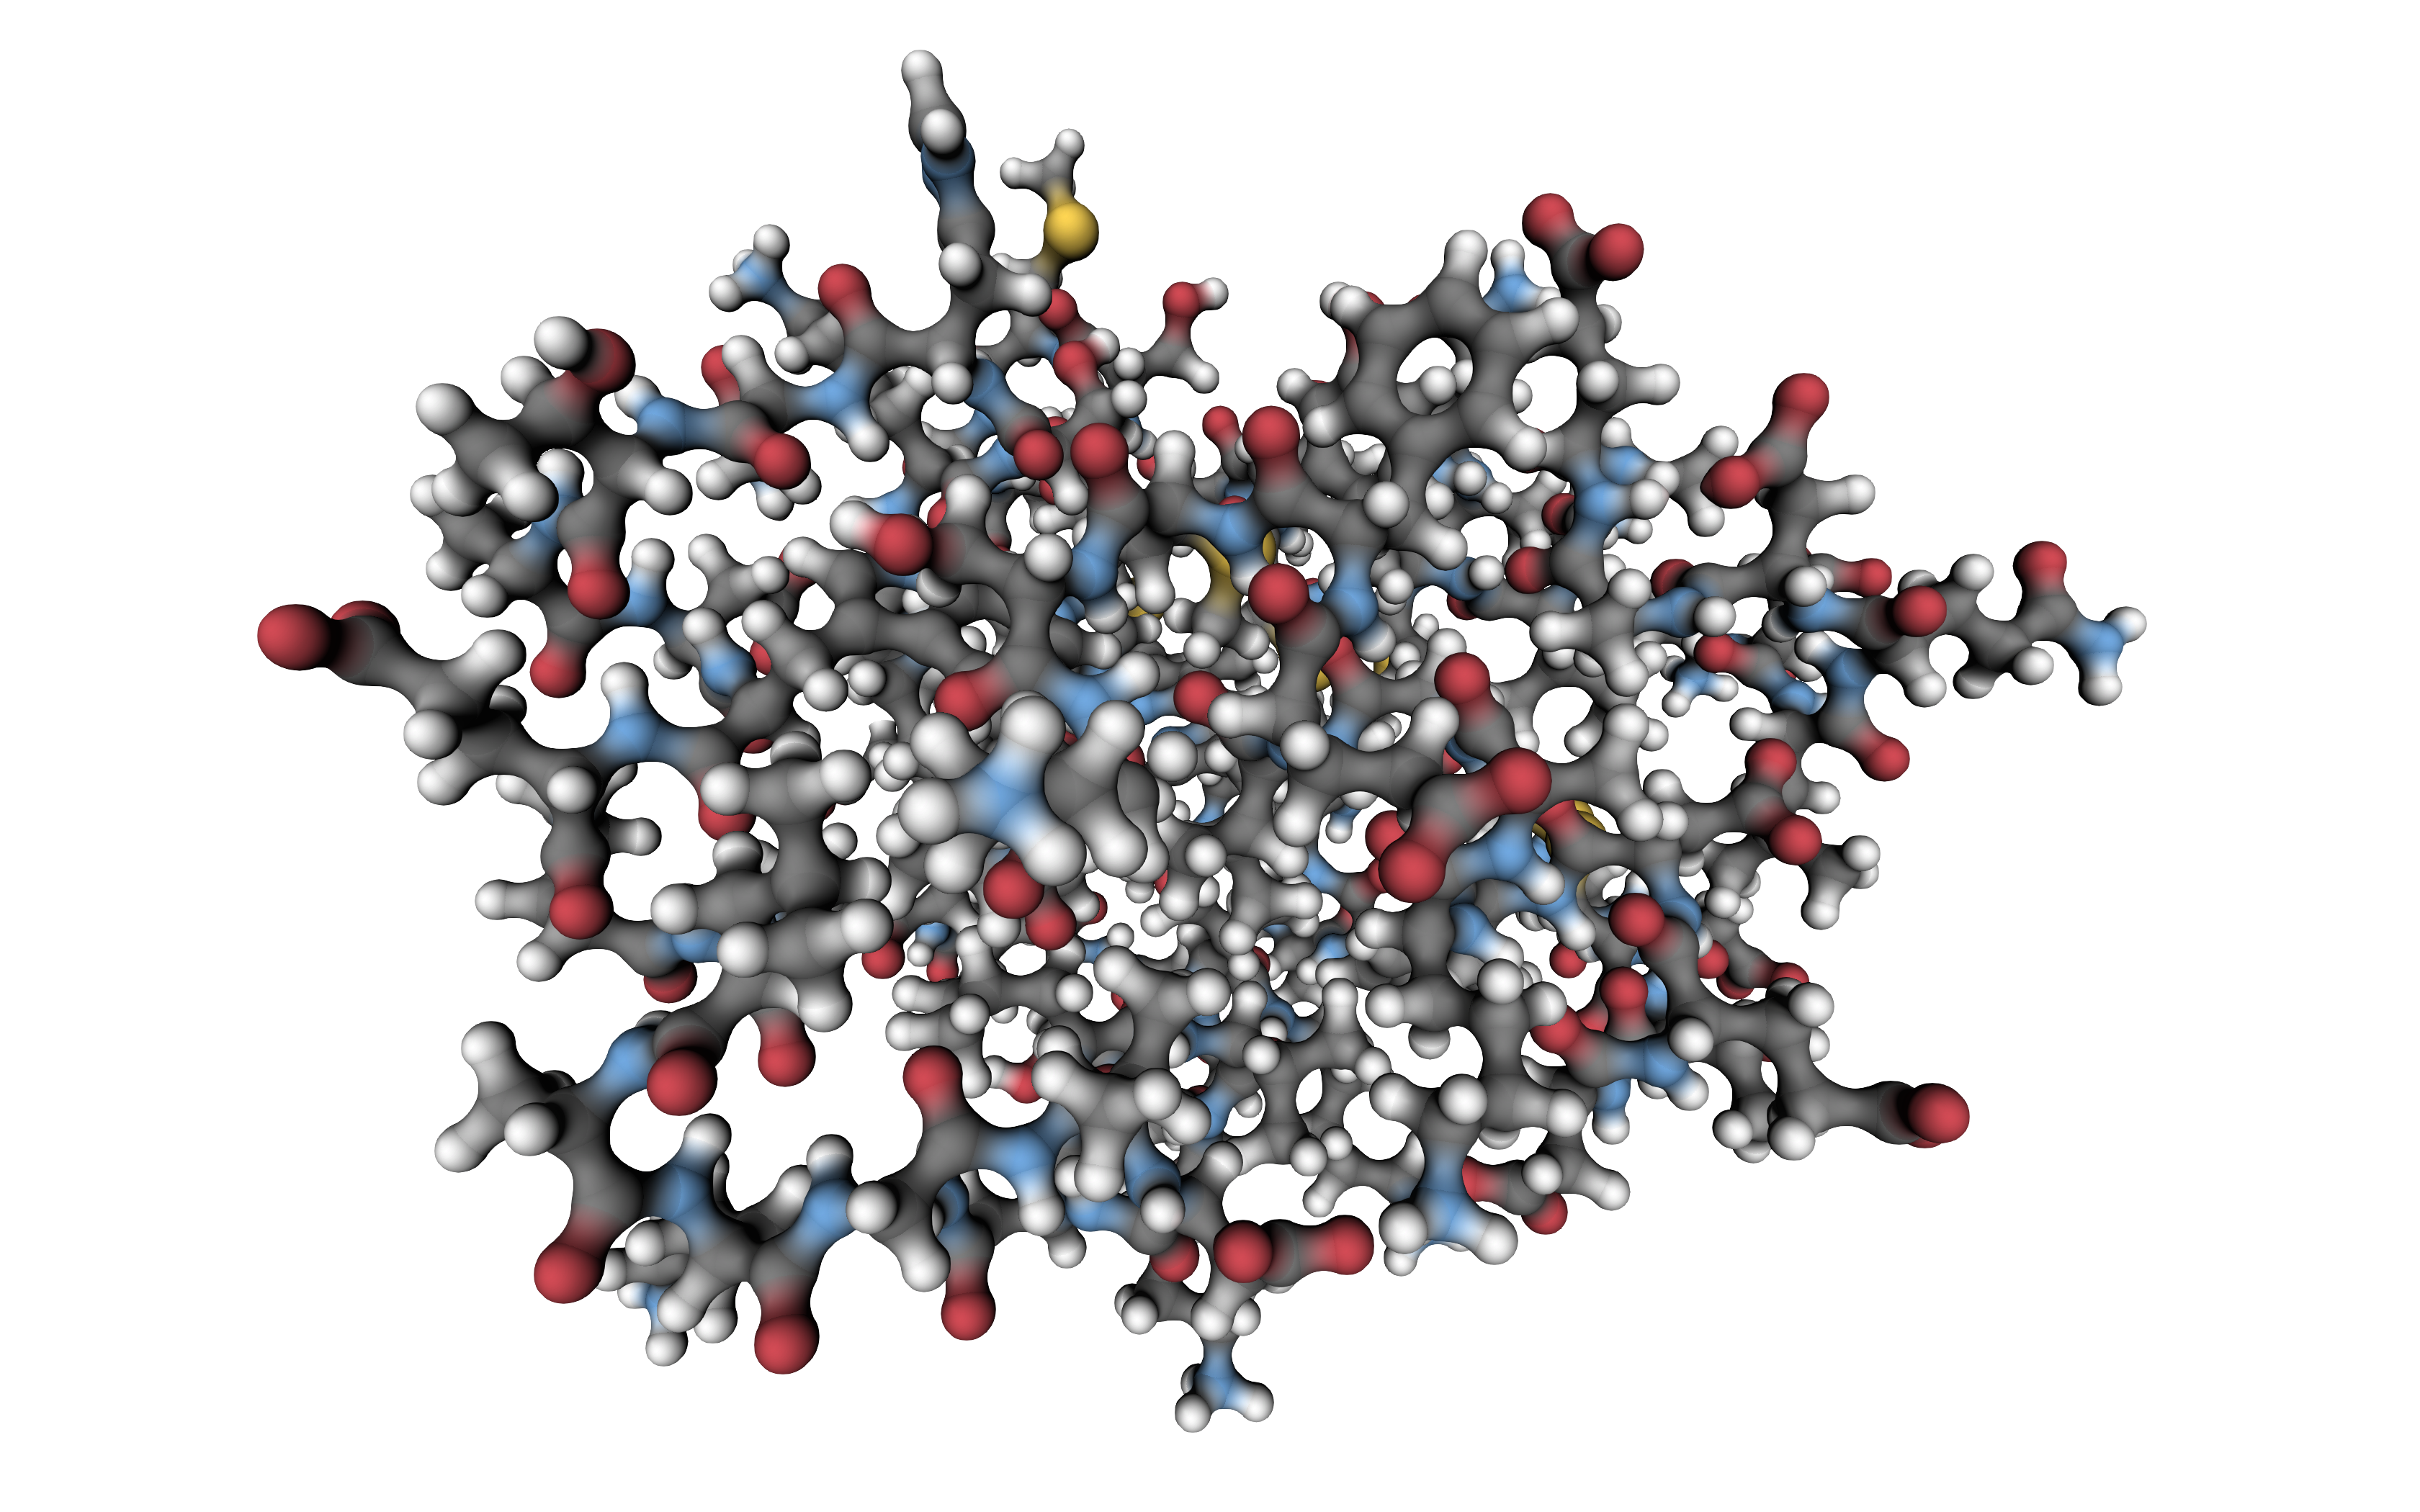
\includegraphics[width=0.60\textwidth]{figures/ch1/1KX2}
		\caption[Une protéine en \emph{Hyperballs}]{Une protéine (\cite{bartalesi2002solution}) représentée avec UnityMol~\cite{doutreligne2014unitymol}. Elle est assez petite (81 acides aminés, vs. $\approx$~30~000 pour la titine), les atomes sont représentés avec un rayon inférieur à leur rayon de vdW, l'occultation est réduite, et les molécules du solvant ne sont pas représentées. Malgré tout, le niveau d'occultation demeure élevé.}
		\label{fig:1KX2}
	\end{figure}
	
	\subsection{Composition}
	Concrètement, une protéine est un une chaîne d'acides aminés, reliés par des liaisons peptidiques, c'est-à-dire des liaisons covalentes entre une fonction carboxyle (–C(O)OH) et une fonction amine (un composé organique dérivé de l'ammoniac dont au moins un atome d'hydrogène a été remplacé par un groupe carboné). Ces chaînes d'acides aminés sont également appelées chaînes polypeptidiques, ou simplement polypeptides.
	
	\subsection{Synthèse}
	Un gène est un brin d'ADN qui \og code \fg{}  une protéine. Dans la cellule, ce brin d'ADN, composé de quatre nucléotides différents : adénine, cytosine, guanine et thymine (A, C, G, T) subit une \emph{transcription} en un brin d'ARN messager, composé également d'adénine, cytosine et guanine, mais d'uracil à la place de la thymine (A, C, G, U). Par exemple, la séquence \texttt{TAGTTCCAGTCAGT} serait transcrite en \texttt{UAGUUCCAGUCAGU}. Si l'ADN a pour fonction de stocker l'information génétique, l'ARN messager permet, comme son nom l'indique, de la communiquer au ribosome, un complexe moléculaire chargé de l'étape de \emph{traduction}.
	
	La traduction se fait selon le \emph{code génétique} illustré par la figure~\ref{fig:geneCode}. Ainsi, à chaque \emph{codon} (non-stop) est associé un acide aminé.
	
	\begin{figure}[htb]
		%\centering
		\begin{subfigure}[t]{0.44\textwidth}
			\centering
			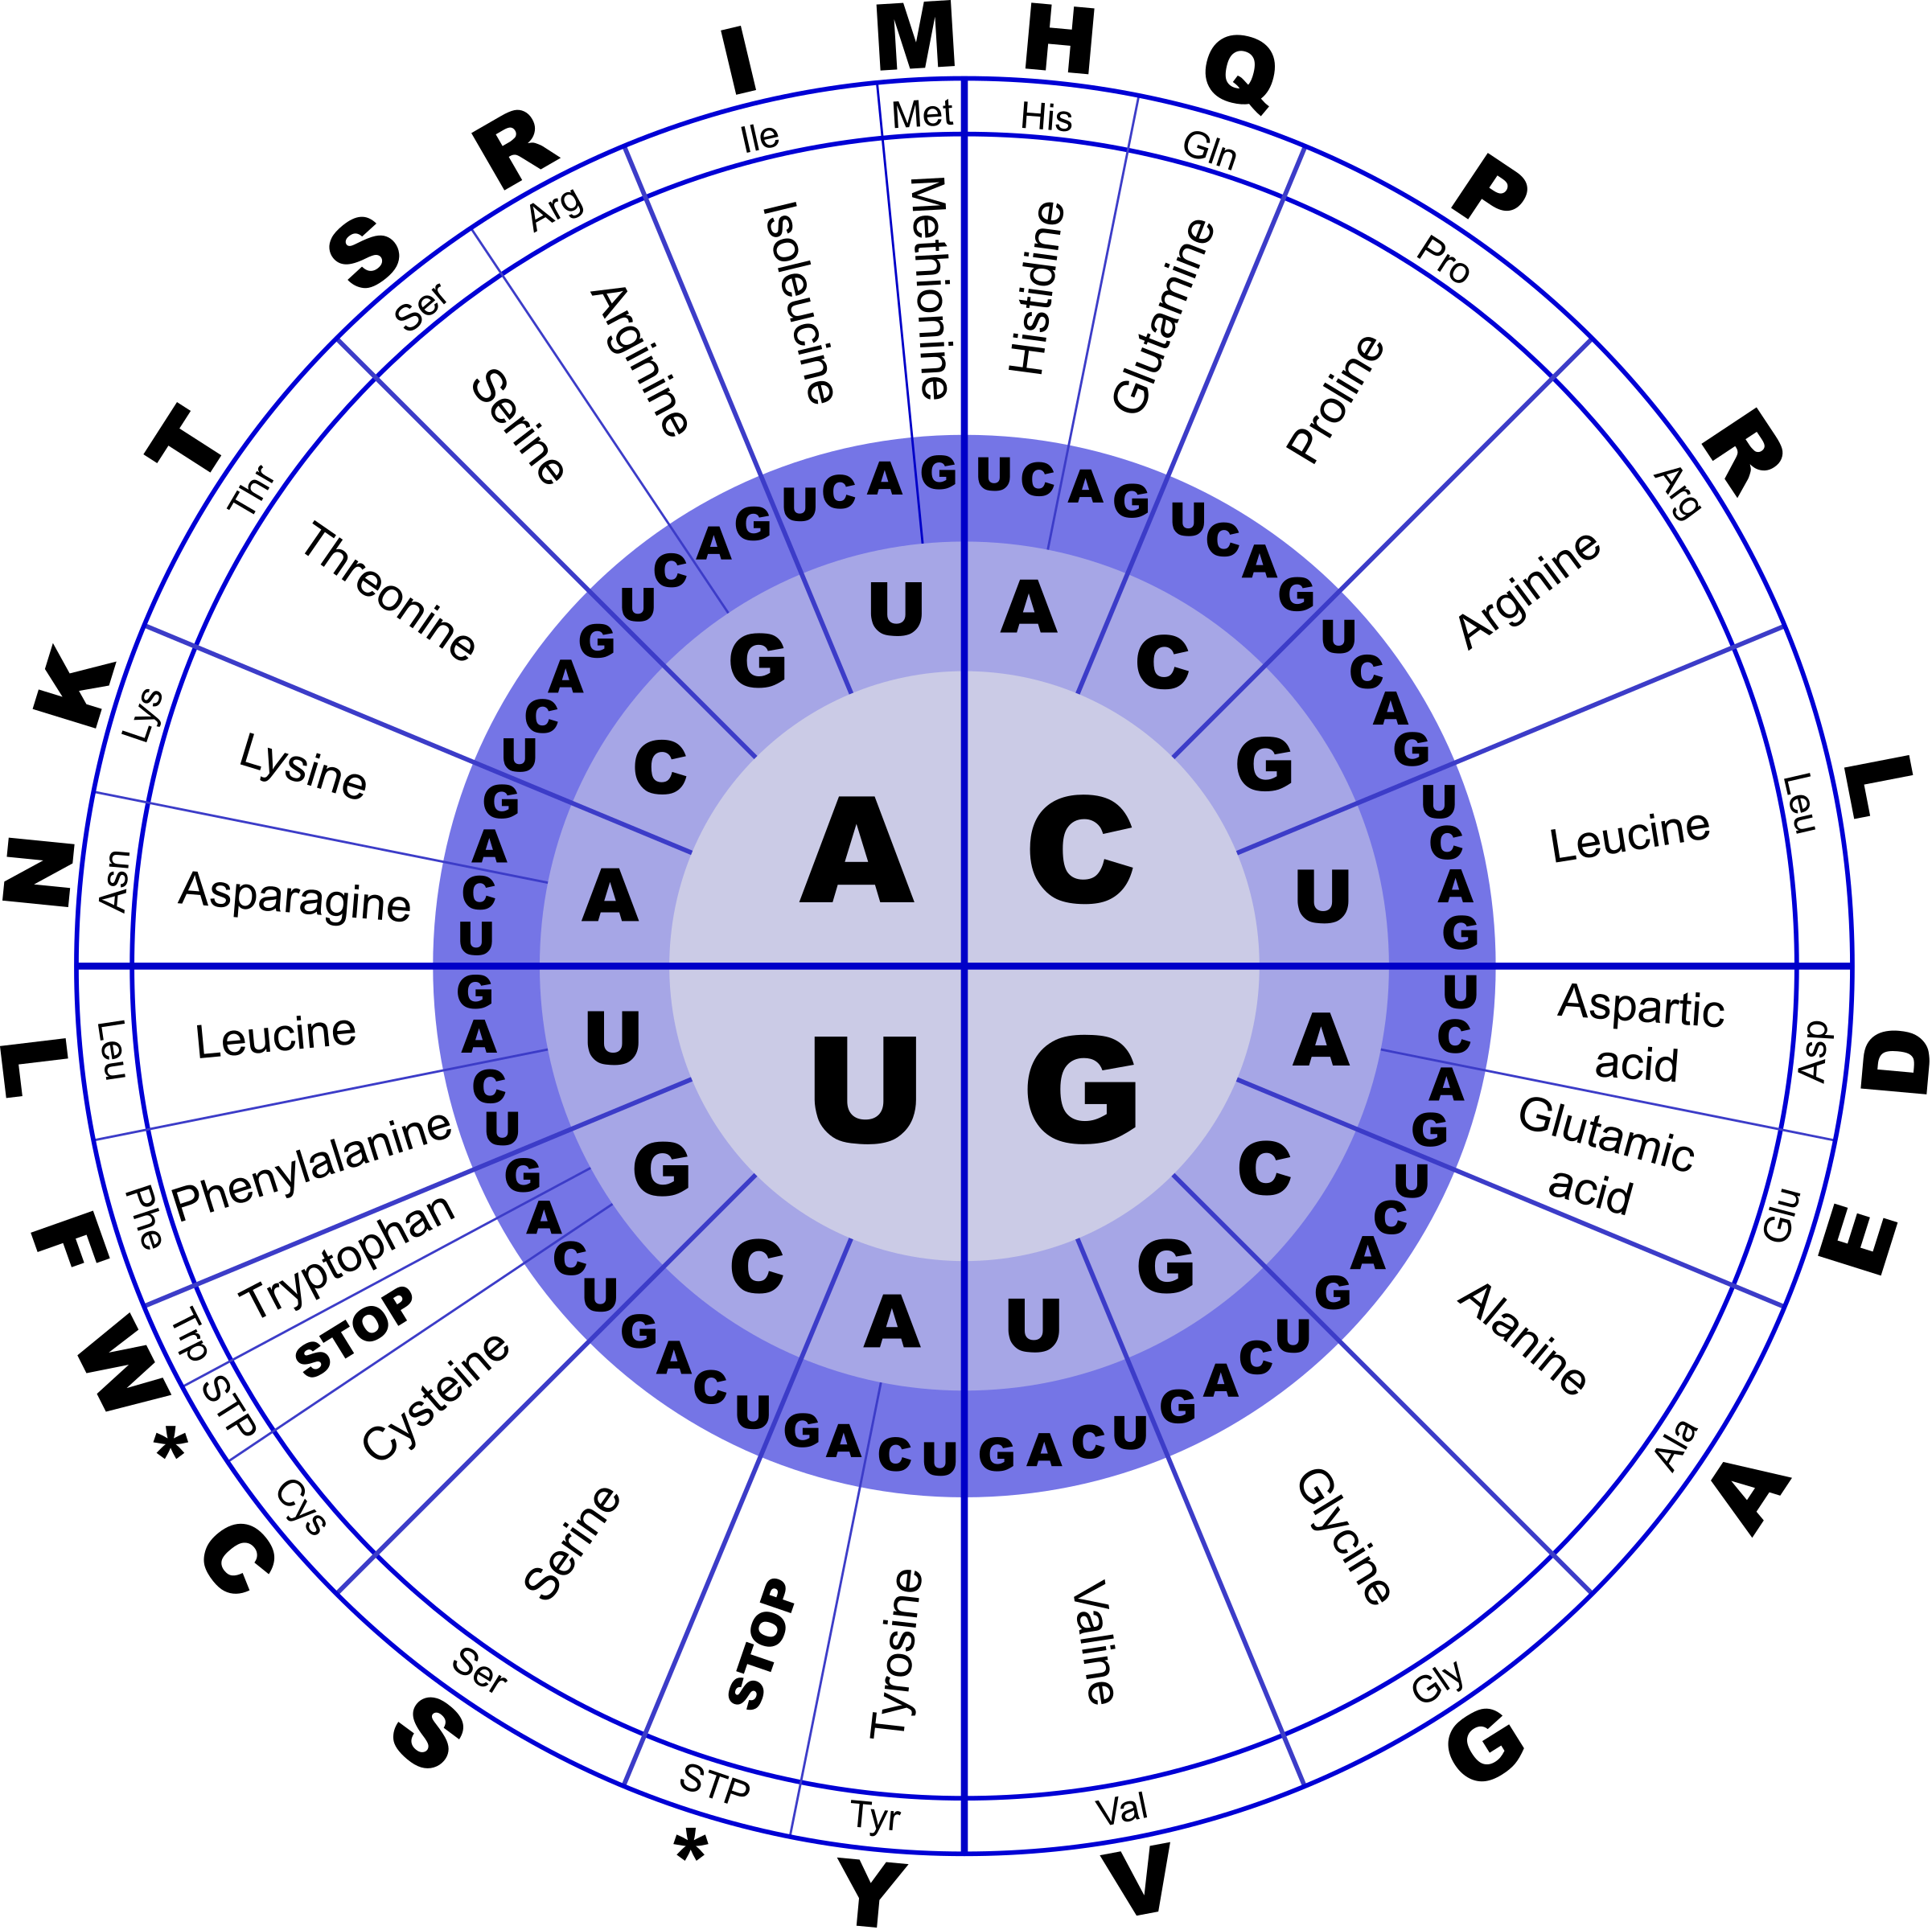
\includegraphics[width=\textwidth]{figures/ch1/geneCode}
			\caption[Le code génétique]{Ce diagramme illustre la correspondance entre un \emph{codon}, c'est-à-dire une suite de trois nucléotides (par exemple \texttt{UCG}) et l'acide aminé associé (dans le même exemple, la serine). On lit un codon du centre vers la périphérie du diagramme. Crédit : J\_{}Alves\footnotemark{}.}
			\label{fig:geneCode}
		\end{subfigure}
		~
		\begin{subfigure}[t]{0.54\textwidth}
			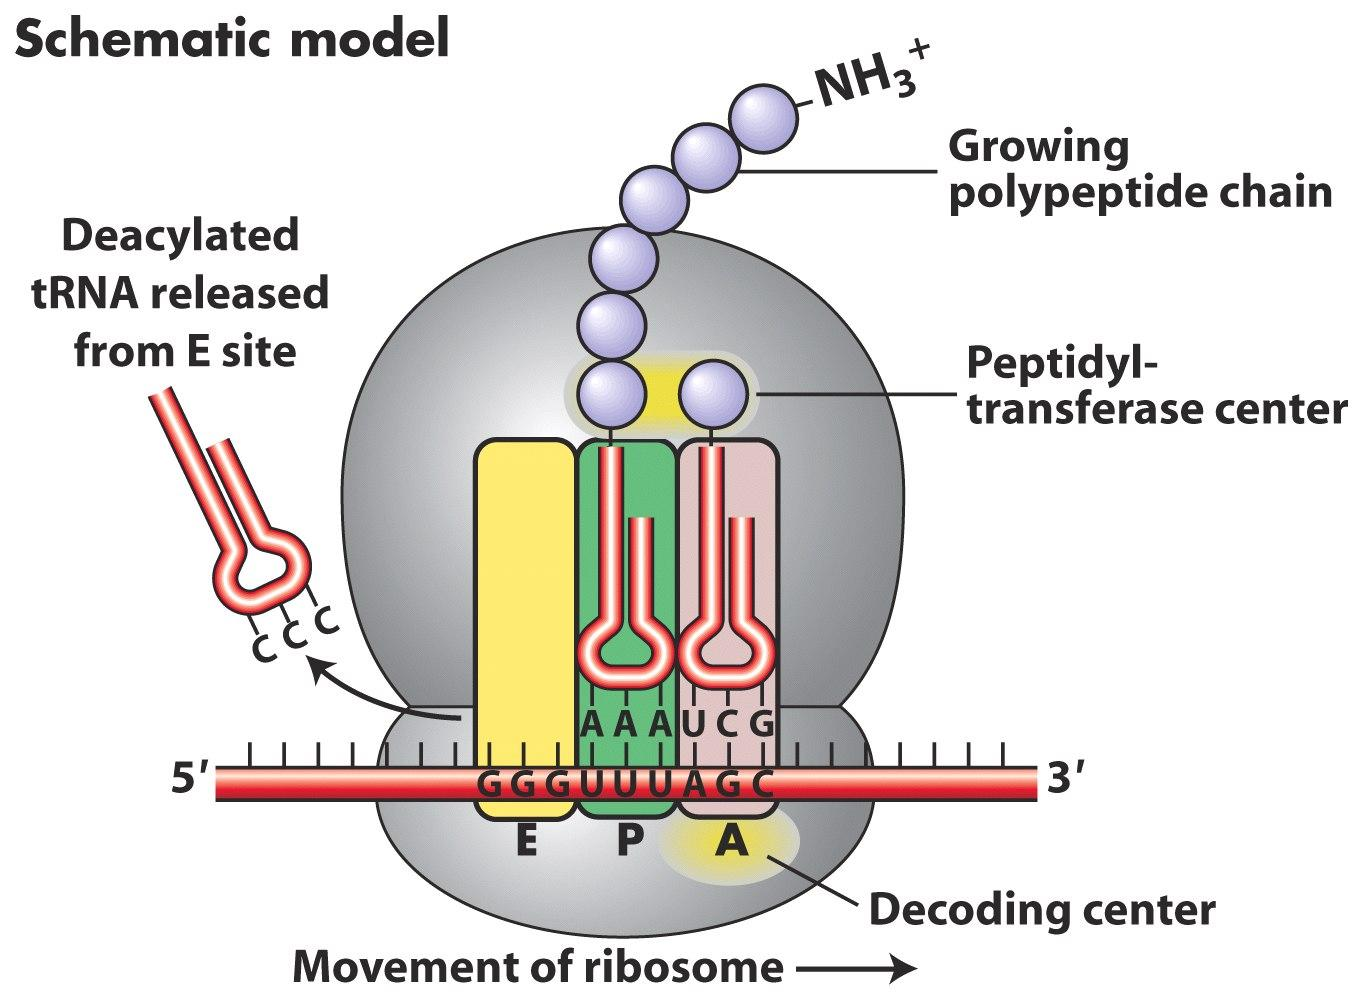
\includegraphics[width=\textwidth]{figures/ch1/translation}
			\caption[Traduction de l'ARN messager en protéine]{Traduction de l'ARN messager et synthèse d'une chaîne polypeptidique. Des ARN de transfert apportent les acides aminés au ribosome qui, en les liant aux bons codons sur le brin d'ARN messager, construit la chaîne polypeptidique dont la protéine finale sera constituée. Crédit : Liberty Voice\footnotemark{}.}
			\label{fig:translation}
		\end{subfigure}
		\label{fig:codeTrans}
		\caption{Code génétique et traduction.}
	\end{figure}
	
	\addtocounter{footnote}{-1}
	\footnotetext{\url{https://openclipart.org/detail/95203/genetic-code-rna}}
	\addtocounter{footnote}{1}
	\footnotetext{\url{http://guardianlv.com/2013/10/naked-mole-rat-longevity-explained-by-higher-translational-fidelity}}
	
	Le ribosome peut ainsi synthétiser une protéine à partir d'un brin d'ARN messager en associant le bon acide aminé à chaque codon, comme l'illustre le montre la figure
	
	\subsection{Structure}
	Les protéines sont décrites selon plusieurs niveaux de structures. On appelle structure primaire, la suite d'acides aminés qui composent la protéine, résultat de la traduction séquentielle d'un gène de l'ADN en protéine selon les règles du code génétique universel, dans lequel à chacun des 64 triplets possibles de nucléotides (A,C,G,T) composant l'ADN, correspond à un acide aminé. À ce niveau de structure, c'est la séquence qui est importante, la protéine étant considérée comme un collier de perles, chaque perle étant un des 22 acides aminées.
	
	Ensuite, pendant et après la synthèse, les protéines s'organisent en 3D pour former des architectures typiques, et cette organisation correspond à la structure secondaire~\cite{foltmann1981protein} qui est en fait une description de la structure tridimensionnelle localement adoptée par un segment de molécule. Cette structure secondaire s'explique par les liaisons hydrogène qui connectent et rapprochent spatialement certains segments, plus précisément entre les groupements amide et carbonyle du squelette peptidique, dans le cas des protéines, et entre les bases nucléiques dans le cas des acides nucléiques (acide désoxyribonucléique, ou ADN, et acide ribonucléique, ou ARN). Parfois, cette définition est assouplie et un segment peut être considéré comme une structure secondaire particulière sur la base des valeurs de certains de ses angles dièdres, indépendamment des liaisons hydrogène. Les algorithmes couramment utilisés pour identifier les structures secondaires incluent DSSP~\cite{kabsch1983dictionary}, \emph{Define}~\cite{richards1988identification}, \emph{Stride}~\cite{frishman1995knowledge} et SST~\cite{konagurthu2012minimum}.
		
	Dans la majorité des cas, une structure secondaire est soit une hélice alpha, soit un feuillet bêta~\cite{pauling1951structure}, soit un segment sans architecture ni contrainte appelé boucle. Dans une représentation dite \og en structures secondaires \fg{} ces segments de molécule sont remplacés par des représentations plus schématiques. Un exemple pour une hélice alpha est présenté dans la figure~\ref{fig:aHelix}, et un exemple pour un feuillet bêta est fourni sur la figure~\ref{fig:bSheet}. L'utilisation de ces schématisations permet de considérablement simplifier la représentation de la molécule finale, comme l'illustre la figure~\ref{fig:4awn_ss}.
	
	\begin{figure}[!htbp]
		%\centering
		\begin{subfigure}[b]{.49\textwidth}
			\centering
			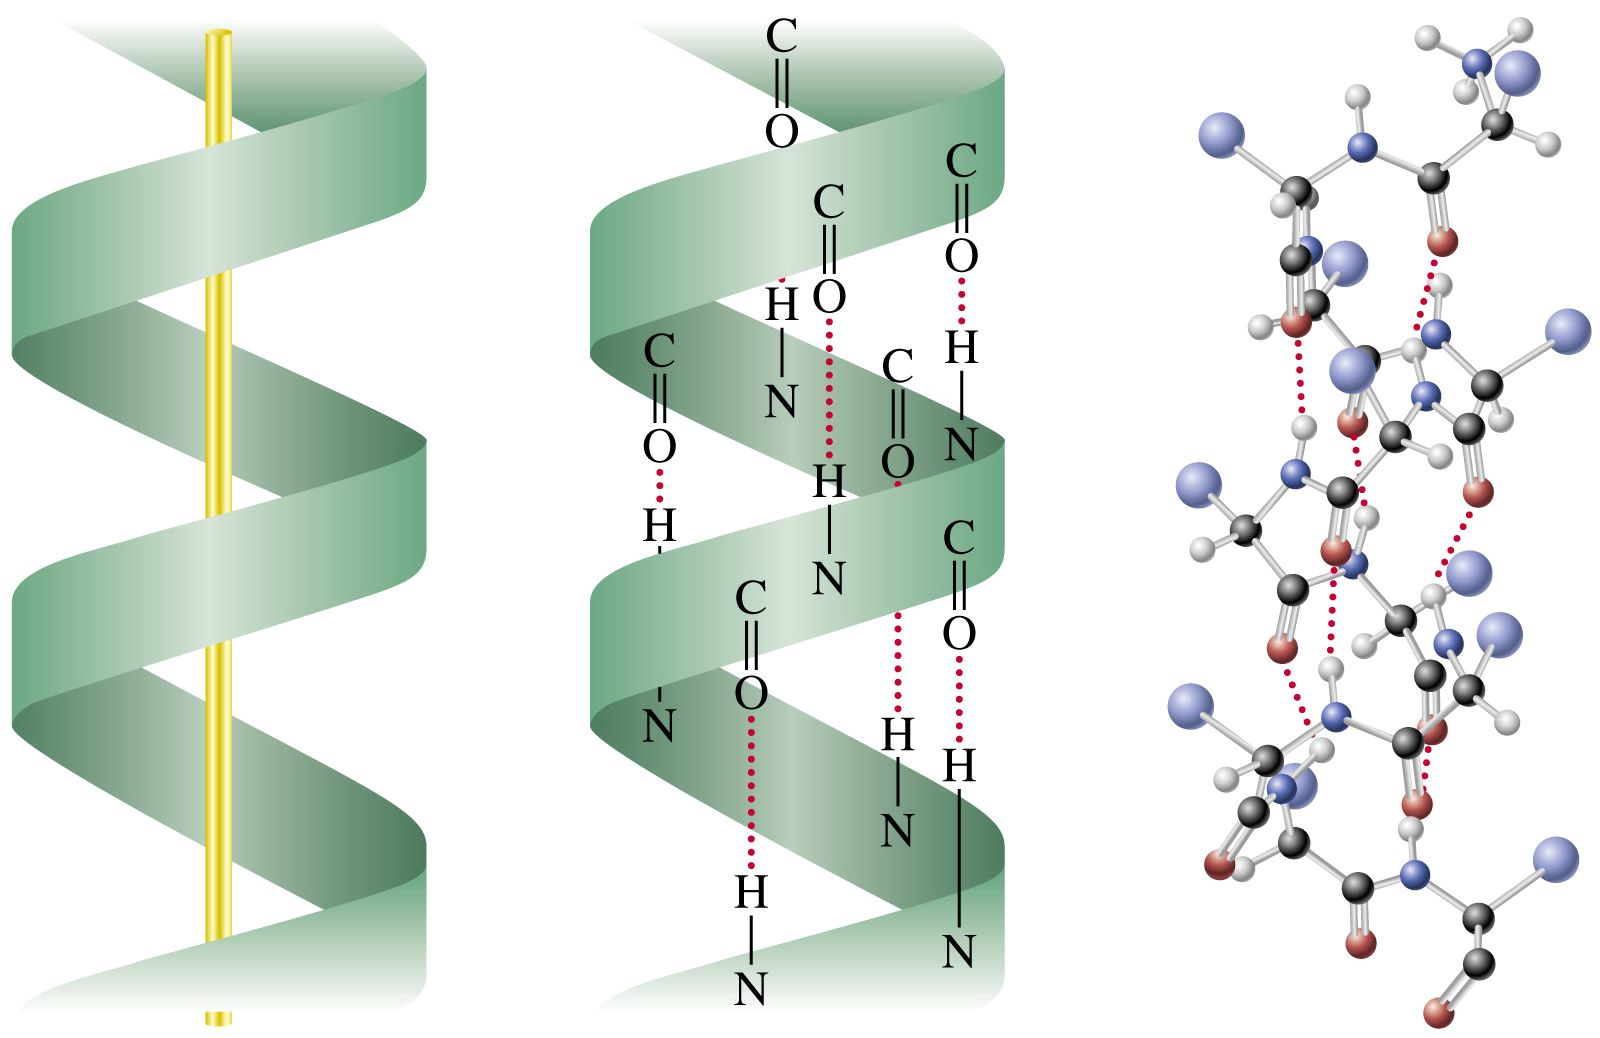
\includegraphics[width=\textwidth]{./figures/ch1/aHelix}
			\caption[Hélices alpha, trois représentations différentes]{Une hélice alpha schématisée (gauche), avec du texte représentant les atomes (centre) et en représentation \og tout atome \fg{} (droite). Lors d'un affichage \og en structures secondaires \fg{} la représentation de gauche est plus courante. Crédit : \emph{Bioinformatics -- An Introduction}, Bioinformatics Lab, AU\footnotemark.}
			\label{fig:aHelix}
		\end{subfigure}
		~
		\begin{subfigure}[b]{.49\textwidth}
			\centering
			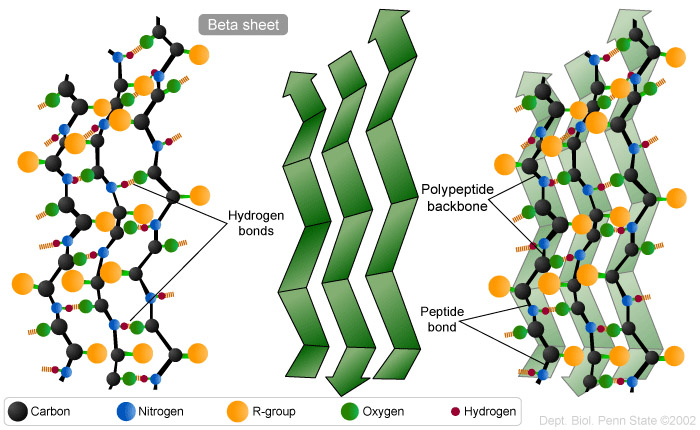
\includegraphics[width=\textwidth]{./figures/ch1/bSheet}
			\caption[Feuillets bêta]{Un feuillet bêta en représentation \og tout atome \fg{} (à gauche), sous forme schématique (au milieu), et en représentation \og tout atome \fg{} mixte (à droite). Lors d'un affichage \og en structures secondaires \fg{} la représentation du milieu est généralement choisie. Crédit : \emph{Department of Biology} -- PSU\footnotemark.}
			\label{fig:bSheet}
		\end{subfigure}
		\caption{Structures secondaires.}
		\label{fig:secStructs}
	\end{figure}
	
	\addtocounter{footnote}{-1}
	\footnotetext{\url{http://bioinfo.au-kbc.org.in/books/bi/1.html}}
	\addtocounter{footnote}{1}
	\footnotetext{\url{https://wikispaces.psu.edu/display/Biol230WCE/Properties+of+Macromolecules+I-Proteins}}
	
	\subsection{Rôles}
	Les protéines sont impliquées dans la plupart des processus biologiques et, de fait, leurs rôles sont extrêmement divers. On peut toutefois les diviser en deux grandes parties : les fonctions cellulaires et les fonctions biochimiques. Les premières définissent le rôle de la protéine dans la cellule ou l'organisme, et peuvent être découpées en cinq groupes~\cite{lodish1995molecular} :
	\begin{enumerate}
		\item Les protéines des structures, qui permettent à la cellule de maintenir son intégrité physique et son organisation dans l'espace. Exemple : le collagène~\cite{di2002mapping}.
		\item Les protéines de transport, qui acheminent les molécules nécessaires aux fonctions cellulaires au sein des cellules, mais aussi à travers les membranes, ou hors des cellules. Exemple : la transferrine~\cite{crichton1987iron}. 
		\item Les protéines régulatrices, qui inhibent ou stimulent l'activité d'autres protéines, ou la transcription de gènes, ce qui permet réguler divers processus biologiques. Exemple : TFIIA~\cite{tan1996crystal}.
		\item Les protéines de signalisation, qui reçoivent les signaux extérieurs (par contact ou liaison avec les molécules qui les transmettent) et assurent leur transmission vers la cellule, ou vers une autre zone de l'organisme. Elles permettent notamment de réagir aux hormones. Exemples : les récepteurs de l'insuline~\cite{gammeltoft1984insulin}.
		\item Les protéines motrices, qui permettent aux cellules ou aux organismes de se mouvoir. Exemple : la myosine~\cite{pollard1973acanthamoeba}.
	\end{enumerate}
	
	\subsection{Modes de représentation}
	Un atome n'est pas un objet au sens où on l'entend communément, dans un contexte macroscopique. S'il est courant de représenter un atome par une sphère, il n'a pas de rayon, de \og coquille \fg{} et ce n'est qu'une représentation schématique de la réalité, utilisée pour communiquer une information. Autour du noyau de l'atome se trouve un nuage électronique où les électrons occupent de manière probabiliste certaines régions de l'espace. Pour représenter ce nuage électronique, on peut procéder comme sur la figure~\ref{fig:helium}.
	
	\begin{figure}[!htbp]
		\centering
		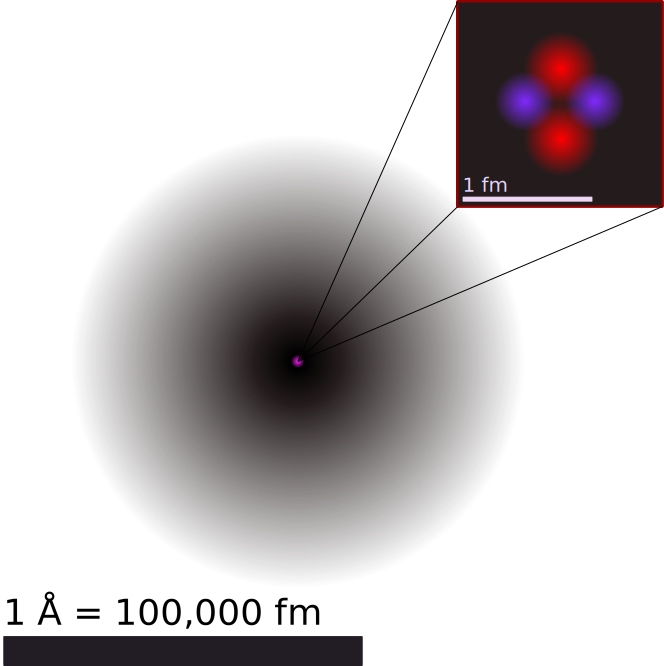
\includegraphics[width=0.40\textwidth]{figures/ch1/helium}
		\caption[Un atome d'hélium avec son nuage électronique]{Un atome d'hélium, avec le noyau en rose et la distribution du nuage électronique en nuances de gris. Le noyau de l'hélium-4 est représenté de façon très schématisée. La barre noire en bas indique l'échelle, et mesure $0,1$ nanomètre. Le dessin d'une \og coque \fg{}  pour représenter un atome sous forme de sphère de rayon fini est un choix arbitraire, dont l'importance pour la sélection d'atomes est déterminante. Crédit : \emph{Wikimedia}.}
		\label{fig:helium}
	\end{figure}
	
	\subsubsection{Points} Le mode de visualisation le plus simple consiste à représenter chaque atome (et uniquement les atomes) par un point tout juste assez gros pour être visible. Les liaisons covalentes ne sont pas représentées. Selon la façon dont elle est mise en œuvre, cette technique de visualisation peut être très performante, et donc garantir un affichage fluide même avec de très nombreux atomes. Elle a de plus l'avantage de minimiser l'occultation des atomes les uns par les autres, du fait de leur petite taille. Cependant, elle communique peu d'informations sur la molécule. En particulier, les liaisons covalentes étant absentes, sa structure même fait défaut. De plus, l'utilisateur peut difficilement se faire une idée de l'espace qu'occupe réellement cette molécule dans son milieu, car chaque atome n'est représenté que schématiquement, par un point bien plus petit que ce que l'on observe sur la figure~\ref{fig:helium}, par exemple.
		
	Enfin, elle rend difficile l'appréciation de la position d'un atome par rapport à ceux qui, dans le plan de l'écran (projeté) se trouvent à proximité, car seule la taille du point permet d'estimer sa distance par rapport à l'observateur. Or, comme les atomes ne font pas tous précisément la même taille, cette appréciation ne peut être que très approximative, même dans le cas où la couleur du point indiquerait la nature de l'atome représenté à un utilisateur connaissant la taille de l'atome en question. La figure~\ref{fig:4awn_points} présente un exemple de cette technique de visualisation. L'on comprend que, si la représentation en points présente certains avantages par rapport à une tâche de sélection, elle est par ailleurs trop limitée pour être appréciée des physico-chimistes ou biologistes souhaitant interagir avec des simulations moléculaires.
	    
	\subsubsection{Bâtons ou réglisse} Un autre mode de visualisation assez simple consiste à représenter uniquement les liaisons covalentes par des traits ou bâtons, juste assez épais pour être clairement visibles, ou par de petits cyclindes ou parallélépipèdes rectangles. Cette représentation est aussi parfois appelée \og réglisse \fg{} ou \emph{licorice}, en anglais. Si les atomes eux-mêmes ne sont pas explicitement représentés, ils se trouvent à l'intersection des liaisons covalentes où à leurs extrémités, et la coloration de ces liaisons indique la nature des atomes qu'elles relient.
		
	Dans une moindre mesure, cette technique de visualisation reprend les avantages de celle en points, puisque le niveau d'occultation, s'il est plus élevé, demeure assez faible. Le coût en ressources de calcul n'est pas nécessairement plus élevé que pour la représentation en points, ce qui permet également d'obtenir de très bonnes performances, même lorsque l'on affiche des systèmes très complexes. Un exemple est fourni dans la figure~\ref{fig:4awn_licorice}.
		
	La visualisation en réglisse, puisqu'elle affiche les liaisons covalentes, représente la structure de la molécule, et la représente même particulièrement clairement. Ses propriétés physico-chimiques peuvent donc être déduites de la représentation, du moins par un utilisateur expert. Par ailleurs, la distance d'un atome par rapport à la caméra est un peu plus facile à apprécier, car l'utilisateur dispose de plus de repères visuels (bien que ceux-ci puissent également occulter totalement l'atome, rendant sa localisation encore plus difficile). Elle partage cependant un inconvénient avec la visualisation en points, puisqu'elle communique à peu près aussi mal l'espace occupé par la protéine, en la réduisant visuellement à son \og squelette \fg{}. Selon les cas, cet inconvénient peut être plus ou moins gênant.
		
	\subsubsection{Boules et bâtons, ou CPK} Une technique de visualisation très courante est appelée \og en boules et bâtons \fg{} (ou \emph{ball-and-stick}, en anglais). Elle est parfois appelée CPK, un peu par abus de langage, en référence aux modèles physiques créés par les chimistes Robert \textbf{C}orey, Linus \textbf{P}auling, et améliorés par Walter \textbf{K}oltun~\cite{corey1953molecular, koltun1965space} ainsi qu'à la convention de couleurs CPK qui est souvent utilisée avec cette représentation. Cette convention est essentiellement caractérisée par l'utilisation du noir pour le carbone, du blanc pour l'hydrogène, du rouge pour l'oxygène, du bleu pour l'azote, du jaune pour le soufre, du violet pour le phosphore, de nuances de vert pour les halogènes (fluore, chlore, brome, iode) et du gris argent pour les métaux.
		
	Ce mode de visualisation, que nous désignerons ci-après par l'appellation \emph{CPK}, représente chaque atome par une sphère, et chaque liaison covalente par un bâton, comme dans la représentation par bâtons. Il s'agit comme dans cette dernière de bien représenter la structure de la molécule, mais en insistant plus sur les atomes. Traditionnellement, ceux-ci sont toutefois représentés par des sphères nettement plus petites que le rayon de van der Waals des atomes (voir le mode suivant).
		
	Outre le fait qu'elle correspond aux modèles physiques CPK, comme celui de la figure~\ref{fig:aspirin}, cette représentation permet de bien visualiser la structure de la molécule et la nature de ses atomes. Naturellement, l'utilisation de sphères implique un degré d'occultation accru par rapport à la représentation en bâtons, mais elle permet aussi d'avoir une meilleure appréciation du volume occupé par la molécule.
		
	Sur ce dernier point, la représentation en boules et bâtons a néanmoins ses limites, puisqu'elle occupe un volume réduit par rapport à certaines références pertinentes d'un point de vue physico-chimique, liées au rayon de van der Waals ou à la densité moléculaire, comme détaillé dans les descriptions des représentations suivantes.
		
	\subsubsection{Sphères de van der Waals} La représentation en sphères de van der Waals (ou vdW) repose sur la notion de rayon de van der Waals. Celle-ci découle elle même de la force de van der Waals~\cite{dzyaloshinskii1961general}. Il s'agit en fait de l'effet combiné de plusieurs forces :
	
	\begin{itemize}
	    \item Les interactions électrostatiques (attractives et répulsives) entre des multipôles permanents, parfois appelées Forces de Keesom~\cite{keesom1915second} ;
		\item L'induction (ou polarisation), c'est-à-dire l'interaction électrostatique attractive entre un multipôle permanent et un multipôle induit, également appelée force de Debye~\cite{debye1913reprinted, debye1929polar} ;
	    \item La dispersion, c'est-à-dire l'interaction électrostatique attractive entre deux multipôles induits, aussi désignée force de London~\cite{eisenschitz1930verhaltnis, london1930theorie, london1937general} ;
		\item La répulsion de Pauli, qui découle du principe d'exclusion de Pauli~\cite{pauli1925zusammenhang}, selon lequel plusieurs électrons (et autres fermions) ne peuvent pas se trouver simultanément dans le même état quantique. En effet, attendu que les électrons de deux atomes ne peuvent pas occuper le même espace simultanément, des atomes dont les nuages électroniques se croisent sont soumis à une force répulsive.
	\end{itemize}
	
	Les logiciels de simulation utilisent fréquemment le potentiel de Lennard-Jones~\cite{lennard1924determination} pour modéliser les forces de van der Waals. Celui-ci peut s'exprimer par ainsi :
	
	$E_{p}\left(r\right) = 4E_{0} \left( \left(\frac{d}{r}\right)^{12} - \left(\frac{d}{r}\right)^{6} \right)$, où $r$ est la distance entre les centres des deux atomes concernés, et $d$ représente la distance pour laquelle le potentiel de Lennard-Jones est nul ; $E_{0}$ est la valeur minimale du potentiel, soit le \og fond \fg{} du puits de potentiel. Comme on l'observe aisément sur la figure~\ref{fig:lennard}, le potentiel admet un minimum, dont on peut déduire un rayon de van der Waals. Ce rayon peut être celui d'une sphère représentant l'atome en question.
 
	C'est le principe de la représentation en sphères de van der Waals, illustrée par la figure~\ref{fig:4awn_VdW}. Ce mode de visualisation a plusieurs avantages. Premièrement, il correspond à une réalité physique, celle des forces de van der Waals. Deuxièmement, il permet d'apprécier le volume occupé par la molécule. Troisièmement, les atomes étant représentés par de grosses sphères, ils sont mieux visibles pour un niveau de zoom donné. De fait, il est plus aisé d'envisager les interactions possibles entre cette molécule et une autre, puisque l'on perçoit mieux les volumes des cavités dans lesquelles d'éventuels ligands\footnotemark{} pourraient venir se loger, et la bonne visualisation des atomes à la surface peut aider à évaluer la probabilité d'un arrimage avec ledit ligand.
	
	\footnotetext{Un ligand est une molécule qui se lie de manière réversible sur une macromolécule ciblée, protéine ou acide nucléique, jouant en général un rôle fonctionnel : stabilisation structurale, catalyse, modulation d'une activité enzymatique, transmission d'un signal. Par exemple, le hème de la myoglobine est un ligand, cf. la figure~\ref{fig:myoglobin}.}
	
	\begin{figure}[!htbp]
		%\centering
		\begin{subfigure}[t]{0.40\textwidth}
			\centering
			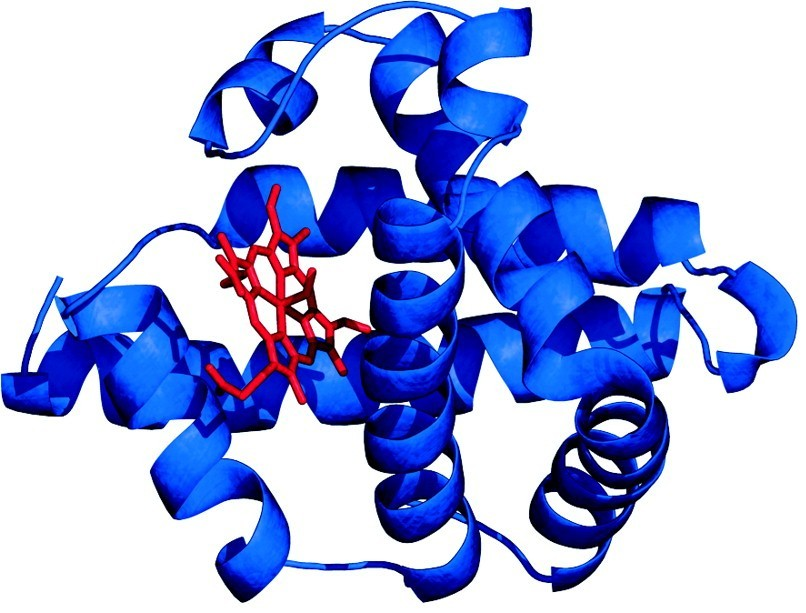
\includegraphics[width=\textwidth]{figures/ch1/myoglobin}
			\caption[Représentation hybride d'une protéine]{Molécule de myoglobine en  structures secondaires, avec son hème en \og tout atome \fg{} (en bâtons rouges). Les niveaux de densité et d'occultation sont donc compris entre ceux de ces deux modes de représentation. Crédit :~\cite{Ordway3441}.}
			\label{fig:myoglobin}
		\end{subfigure}
		~
		\begin{subfigure}[t]{0.58\textwidth}
			\centering
			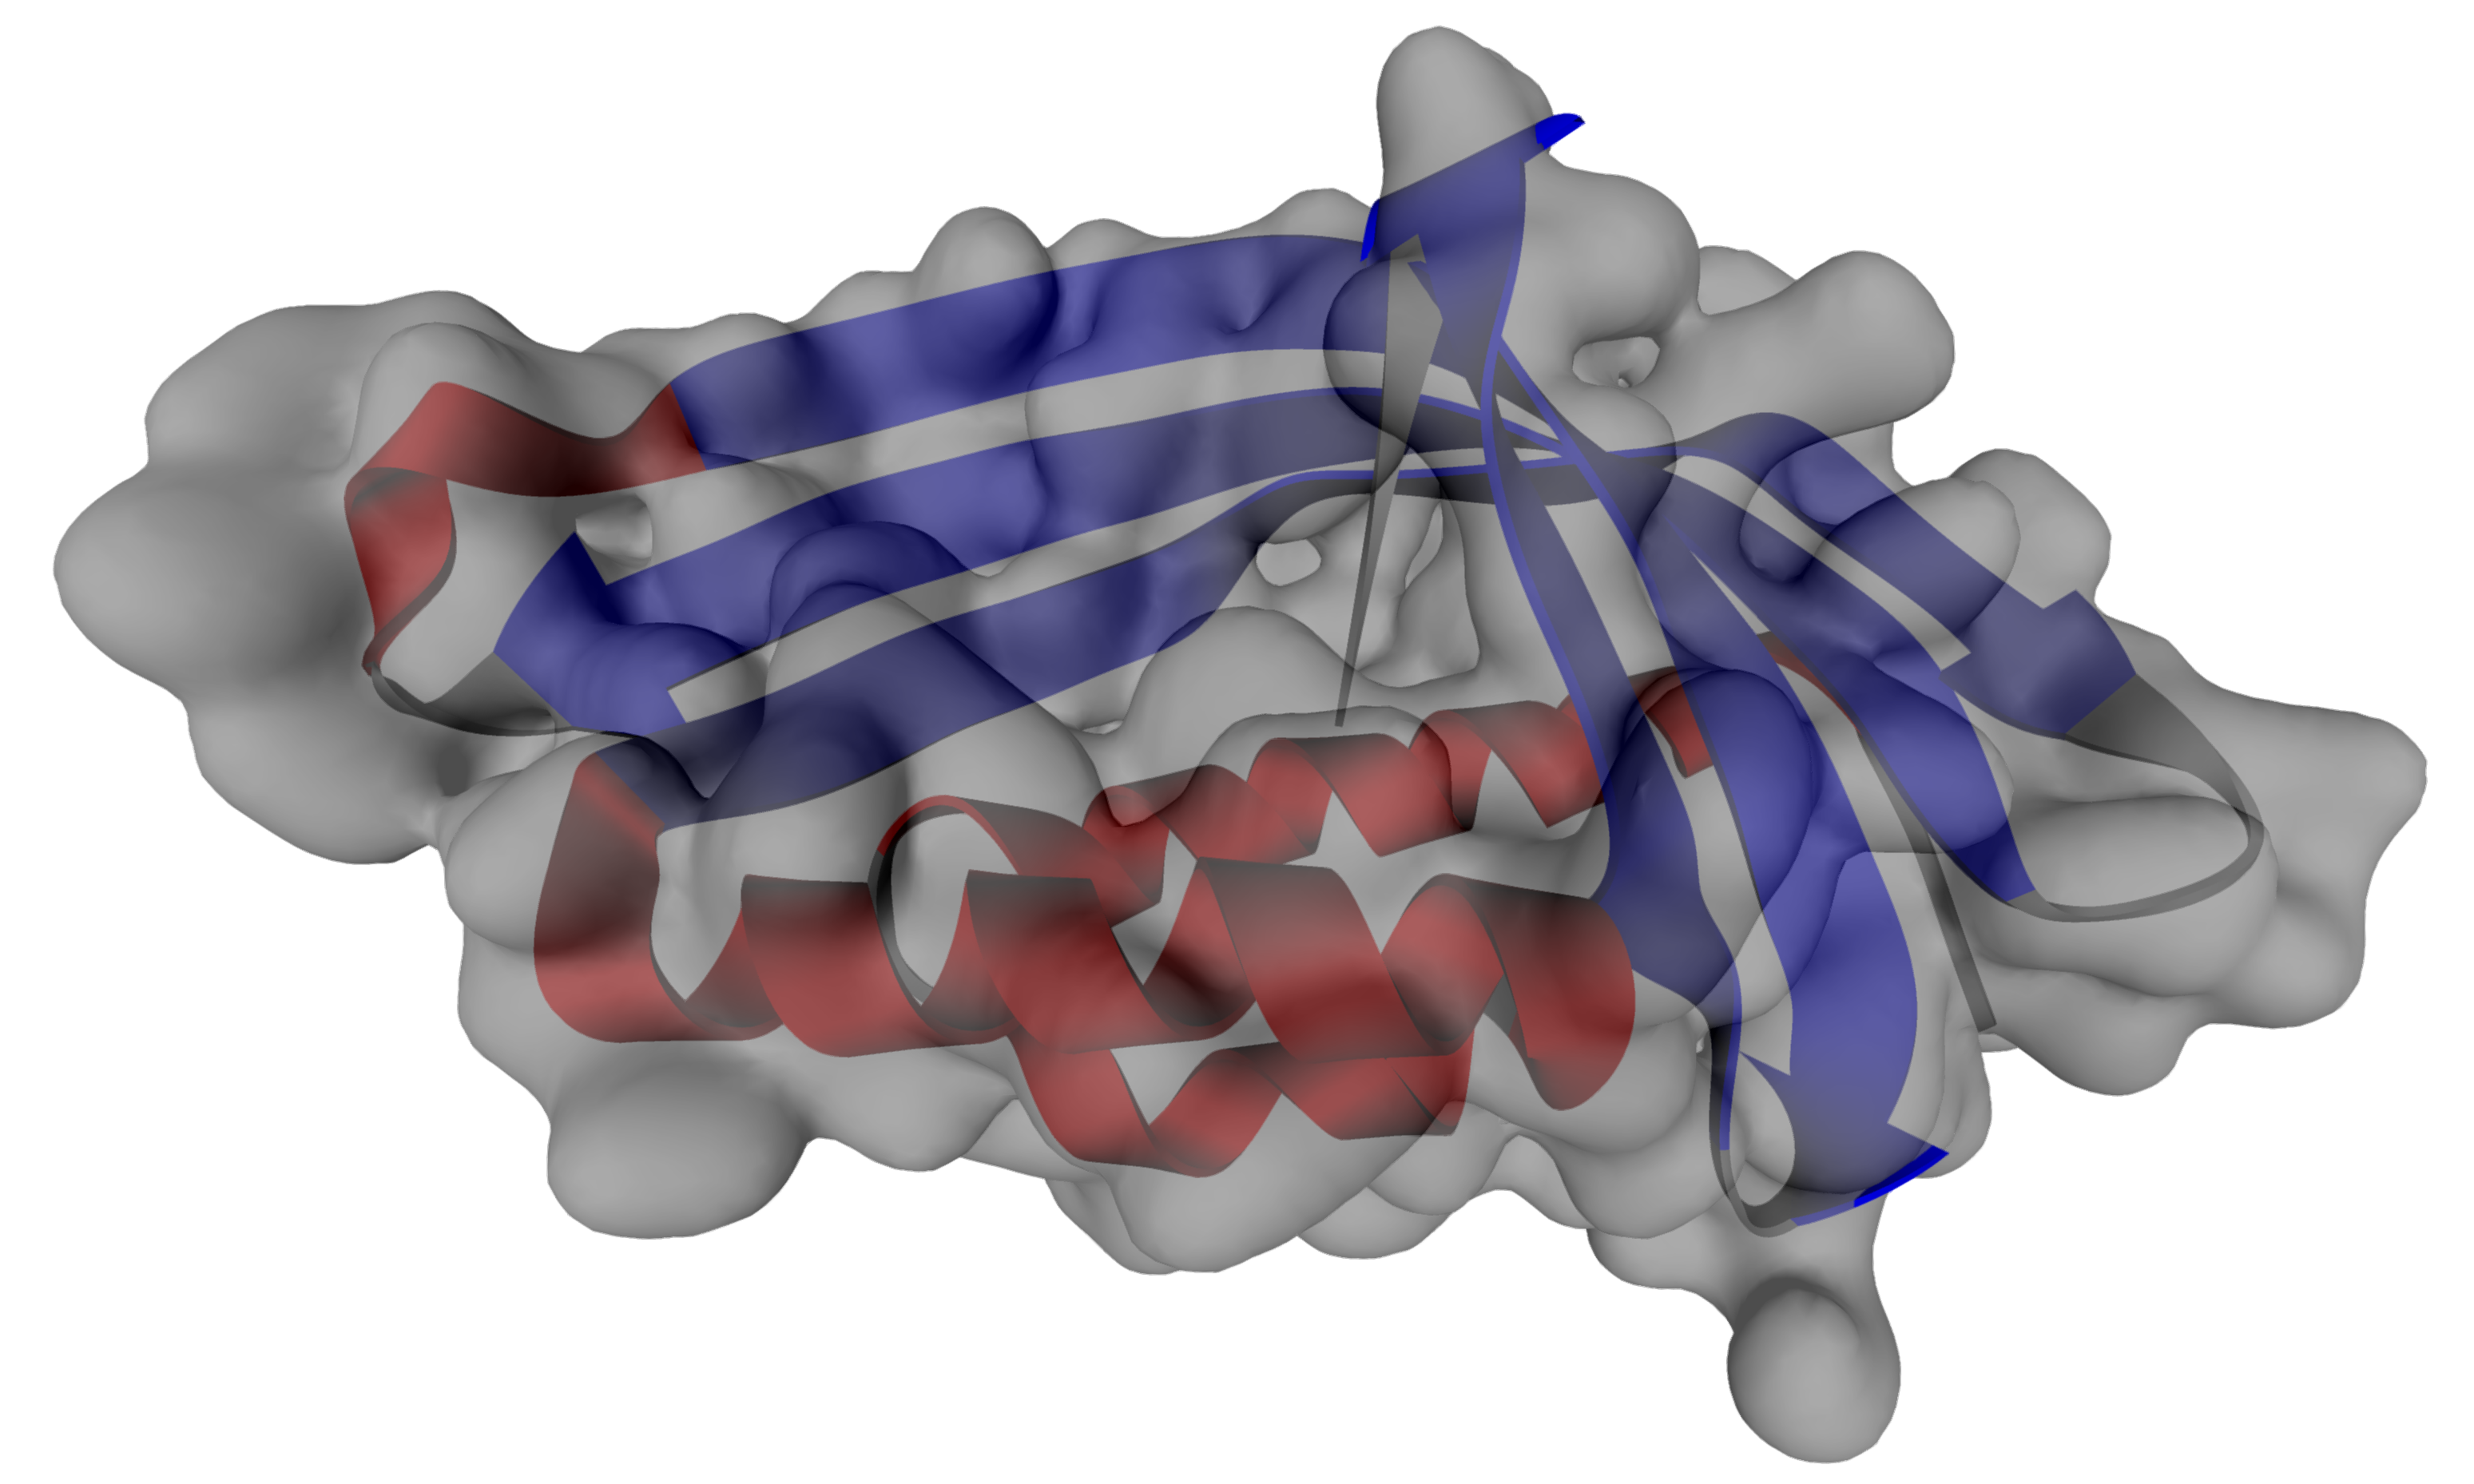
\includegraphics[width=\textwidth]{figures/ch1/transSS}
			\caption[Surface semi-transparente et structures secondaires]{Représentation hybride d'une protéine de chloroplaste, avec une isosurface de densité semi-transparente et les structures secondaires. On peut donc apprécier à la fois le volume occupé par la molécule et les aspérités de sa surface, mais aussi sa structure interne et certaines de ses propriétés physico-chimiques. Image générée avec \emph{UnityMol} à partir d'une structure de la \emph{Protein Data Bank}.}
			\label{fig:transSS}
		\end{subfigure}
		\label{fig:hybrid}
		\caption{Représentations hybrides de molécules.}
	\end{figure}
		
	Cependant, les liaisons covalentes sont totalement occultées, et il est seulement possible de les \og deviner \fg{} à partir de l'emplacement des atomes et grâce aux lois de la chimie. La structure de la molécule est donc beaucoup moins claire qu'en représentation CPK, par exemple. De plus, les atomes sont si gros qu'ils occultent totalement ceux qui sont derrière eux. De fait, l'intérieur de la molécule devient totalement invisible. Si sa surface est mieux représentée, sa structure interne est entièrement occultée. C'est plus gênant encore lorsque les atomes d'hydrogène sont affichés, ce qui n'est pas le cas sur la figure~\ref{fig:4awn_VdW} --- il est courant de les omettre, par souci de clarté. Selon la mise en \oe{}uvre logicielle de cette représentation, elle peut être coûteuse en ressources de calcul, même si des solutions efficaces existent. En mouvement, la grande taille des atomes a l'avantage de diminuer leur mouvement relatif, c'est-à-dire leur mouvement par rapport à eux-mêmes.
		
	Les sphères de van der Waals ne sont pas une mauvaise option pour visualiser (ou interagir avec) une simulation de dynamique moléculaire, à condition que l'objet d'intérêt principal soit superficiel, et donc bien visible. La grande taille des cibles peut être un avantage, même s'il y a un certain degré d'interpénétration entre elles. Cette représentation constitue donc un cas d'application notable pour une technique de sélection de cibles mobiles.
	
 	\begin{figure}[!htbp]
 		\centering
 		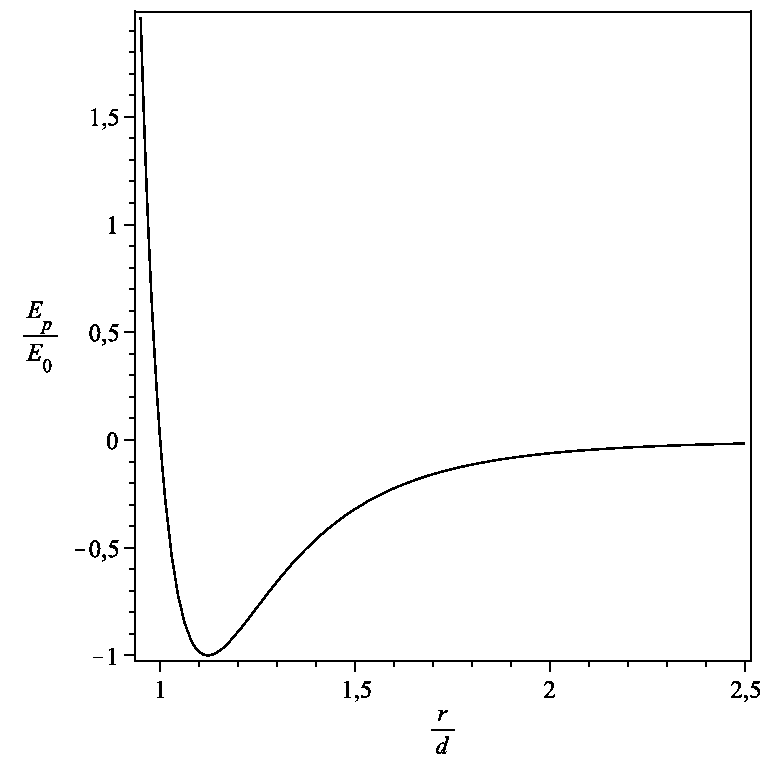
\includegraphics[width=0.46\textwidth]{figures/ch1/lennard-jones}
		\caption[Représentation graphique du potentiel de Lennard-Jones]{Représentation graphique du potentiel de Lennard-Jones, en fonction du rapport $r/d$ entre la distance interatomique réelle et celle pour laquelle le potentiel s'annule. Le potentiel admet un minimum en $r/d = 2^{1/6}$, soit environ $1,12$ ; ce minimum correspond au rayon de van der Waals. Crédit : \emph{Wikimedia}.}
 		\label{fig:lennard}
 	\end{figure}
	
	\subsubsection{\emph{Hyperballs}} La technique de visualisation de molécules appelée \emph{Hyperballs}~\cite{chavent2011gpu} se fonde sur une représentation analytique des atomes et des liaisons covalentes. Leurs surfaces sont décrites par des équations, des rayons sont lancés vers les atomes, et il s'agit ensuite de résoudre des équations d'intersection entre les rayons et les surfaces.
		
	Les \emph{Hyperballs} présentent de nombreux avantages. Sur le plan purement technique, leur mode de représentation analytique permet, au contraire des maillages de points (\emph{meshes}, en anglais), d'éviter d'avoir à gérer un très grand nombre de points et de triangles. De plus, quel que soit le niveau de zoom, les surfaces des sphères et des liaisons covalentes (représentées par des hyperboloïdes) demeurent parfaitement lisses. Avec des maillages, il est nécessaire d'avoir un grand nombre de triangles pour maintenir l'illusion de la rotondité du modèle lorsqu'il est observé de près.
	
	En réalité, les illustrations fournies jusqu'ici pour la représentation en points, en bâtons, en boules et bâtons, et en sphères de van der Waals ont toutes été produites avec des \emph{Hyperballs}, simplement en jouant sur leurs paramètres. Cette grande flexibilité rend cette technique particulièrement avantageuse, surtout compte tenu des performances de premier ordre qu'elle offre~\cite{chavent2011gpu}.
		
	Au-delà de sa flexibilité, cependant, elle a l'avantage de permettre une représentation originale, avec des liaisons représentées par des hyperboloïdes. En jouant sur la courbure de ces hyperboloïdes, on peut communiquer des informations sur la nature de la liaison, par exemple sur la quantité d'énergie nécessaire à sa rupture. Si cette quantité est faible, on peut représenter la liaison par une hyperboloïde très \og creusée \fg{}, donnant l'impression d'être sur le point de rompre.
		
	Enfin, les \emph{Hyperballs}, utilisées de la façon la plus \og classique \fg{} ou \og canonique \fg{} présentent des hyperboloïdes partiellement creusées, comme sur la figure~\ref{fig:4awn_HB}. Cette représentation est souvent appréciée pour ses qualités esthétiques, certes subjectives. D'un point de vue plus objectif, la représentation en \emph{Hyperballs} canoniques présentent à peu près les mêmes caractéristiques que la représentation en boules et bâtons. Les dimensions sont proches, même si les formes diffèrent. Les liaisons sont un peu plus épaisses près des atomes, et comparables, voire un peu plus fines au milieu. De fait, la perception de la structure de la molécule et de ses propriétés, ainsi que le niveau d'occultation visuelle, sont assez comparables. Par conséquent, la représentation en \emph{Hyperballs} canoniques est un cas d'application aussi pertinent pour la sélection de cibles mobiles que la représentation CPK, voire plus, car les bonnes performances des \emph{Hyperballs} permettent de gérer de très gros systèmes plus facilement.
	
	\subsubsection{Surface accessible au solvant et surface de Connolly}
	Plutôt que de représenter les atomes d'une molécule, ou ses liaisons covalentes, ou sa structure interne de façon schématique, il est possible de représenter sa \og surface \fg{}. Attendu qu'une molécule n'est pas un objet macroscopique, le concept de surface est nécessairement plus abstrait, et il convient donc de préciser de quoi il s'agit. On peut en effet définir la surface moléculaire de plusieurs façons.
		
	Un définition très courante est la surface de Connolly~\cite{connolly1983analytical}, parfois également appelée \emph{solvent excluded surface} dans la littérature anglo-saxonne. Il s'agit de l'ensemble des points auxquels la molécule et \og le solvant \fg{} (généralement une sphère représentant une molécule d'eau) peuvent entrer en contact, où le contact est défini par le rayon de van der Waals.
	
	\begin{figure}[!htbp]
		\centering
		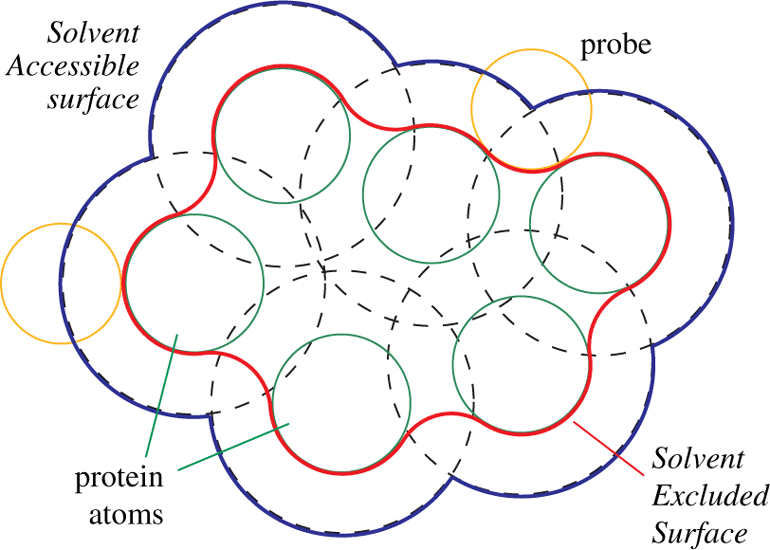
\includegraphics[width=0.56\textwidth]{figures/ch1/connolly}
		\caption[Surface de Connolly et accessible au solvant]{Surface de Connolly. Une sonde (cercles jaunes) est \og roulée \fg{} sur les atomes (verts) de la molécule, et son tracé est conservé en rouge : c'est la surface de Connolly. La surface tracée par le centre de la sonde est dite accessible au solvant. Cet algorithme est aussi appelé \emph{rolling ball}~\cite{shrake1973environment, connolly1983analytical, connolly1993molecular}. Crédit :~\cite{krone2009interactive}.}
		\label{fig:connolly}
	\end{figure}
	
	La figure~\ref{fig:connolly} illustre plus clairement ce principe. Une autre surface très courante est la surface accessible au solvant~\cite{lee1971interpretation}, définie par l'ensemble des points parcourus par le centre de la sphère représentant le solvant quand elle est en contact avec la molécule. C'est également illustré par la figure~\ref{fig:connolly}. Enfin, la figure~\ref{fig:4awn_ses} montre une protéine entière représentée par sa surface de Connolly.
		
	\subsubsection{Isosurface de densité} On peut également représenter une molécule par sa surface en se fondant sur un seuil de densité moléculaire. On calcule, dans une grille tridimensionnelle d'une résolution arbitraire, la densité en chaque case --- on construit un champ scalaire. Ensuite, on choisit arbitrairement un seuil de densité, et l'on trace une isosurface de densité à partir de ce seuil. On utilise généralement pour ce faire l'algorithme des \emph{marching cubes}~\cite{lorensen1987marching}.	L'isosurface de densité $D$ correspond à l'ensemble des points de l'espace dont la densité moléculaire vaut $D$.
	
	Outre le fait qu'elle représente une grandeur physique concrète, l'isosurface de densité a l'avantage d'être relativement rapide à calculer. En effet, l'algorithme \emph{QuickSurf}~\cite{krone2012fast, roberts2013lattice, stone2013early, stone2013gpu, stone2014gpu, sener2014visualization}, par exemple, permet de calculer une isosurface de densité suffisamment vite pour la recalculer en temps réel lors d'une simulation de dynamique moléculaire. Cet algorithme est conçu pour être exécuté sur un GPU (un processeur graphique, particulièrement adapté aux calculs très parallèles) ce qui améliore ses performances d'un à deux ordres de grandeur. Il permet de plus d'ajuster plusieurs paramètres : la résolution spatiale générale, le rayon des atomes (utilisé pour générer la grille de densité, par somme de gaussiennes 3D), l'isovaleur de densité voulue, la résolution de la grille de densité, et la distance de coupure utilisée pour la gaussienne associée à chaque atome\footnote{\url{http://www.ks.uiuc.edu/Research/vmd/current/ug/node73.html}}.
	
	Du fait des performances de cet algorithme et de sa souplesse, les isosurfaces de densité représentent un cas d'application intéressant. En effet, elles sont assez couramment utilisées en simulation de dynamique moléculaire, et présentent des caractéristiques très distinctes des modèles de représentation atomiques. Contrairement à ces derniers, elles ne présentent pas de (dizaines ou centaines) de milliers de cibles distinctes, mais un seul objet continu. De fait, au premier abord elles ne semblent pas nécessiter d'assistance à la sélection. Cependant, les nombreuses aspérités d'une isosurface, attendu qu'elles correspondent à celles de la molécule, peuvent être considérées comme des cibles distinctes, à condition d'avoir une méthode pour les distinguer. Cette méthode pourrait éventuellement être fondée sur des critères de concavité et convexité. Si l'on considère chaque sous-ensemble convexe d'une surface de densité avec un seuil élevé, par exemple, on aboutit à plusieurs dizaines de cibles potentielles ; et ce pour une protéine de taille relativement réduite (par exemple 2000 atomes, quand certaines protéines en comptent des dizaines de milliers). On peut également considérer les sous-ensembles concaves comme des cibles, car ils peuvent représenter des cavités ou tunnels\footnotemark{} dignes d'intérêt.
	
	\footnotetext{Les cavités et tunnels des protéines sont critiques pour la compréhension de phénomènes tels que la liaison de ligands, le transport moléculaire ou la catalyse enzymatique~\cite{paramo2014}.}
	
	On constate donc qu'une isosurface de densité peut présenter de nombreuses cibles mobiles, avec toutefois un niveau d'occultation réduit, puisque l'intérieur de la molécule n'est pas représenté. Les aspérités situées à \og l'arrière \fg{} de la molécule sont cependant totalement occultées. De plus, la représentation en isosurface est particulièrement prisée pour l'arrimage\footnote{\emph{Docking}, en anglais} de protéines, qui implique au moins deux molécules et parfois beaucoup plus. Avec de nombreuses molécules, le nombre de cibles potentielles peut donc devenir très élevé, de même que la quantité de mouvement, puisqu'il faut ajouter au mouvement d'une aspérité d'une surface par rapport à elle-même le mouvement de toute la surface par rapport à l'environnement.
	
	\subsubsection{Autres techniques de représentation}
	La liste des techniques de représentation fournie ci-dessus ne saurait être considérée comme exhaustive. En effet, les logiciels de visualisation moléculaires sont nombreux, et les possibilités qu'ils offrent le sont encore plus. Des programmes couramment utilisés, tels que \emph{UnityMol}~\cite{kouyoumdjian2013umol, kouyoumdjian2014game, doutreligne2014unitymol, martinez2017vizmol}, VMD~\cite{humphrey1996vmd}, \emph{PyMol}~\cite{delano2002pymol}, \emph{QuteMol}~\cite{tarini2006ambient, tarini2006qutemol}, \emph{Chimera(X)}~\cite{pettersen2004ucsf, goddard2017ucsf}, ~\emph{Yasara}~\cite{krieger2014yasara}, \emph{LigandScout}~\cite{wolber2005ligandscout} ou \emph{Jmol}~\cite{herraez2006biomolecules} proposent des options très diverses. En outre, les divers modes de représentation proposés par ces outils peuvent être combinés librement, comme sur la figure~\ref{fig:transSS}.
	
	
	\newcommand{\subImgW}{0.32\textwidth}
	\begin{figure}[!htbp]
		%\centering
		\begin{subfigure}[t]{\subImgW}
			\centering
			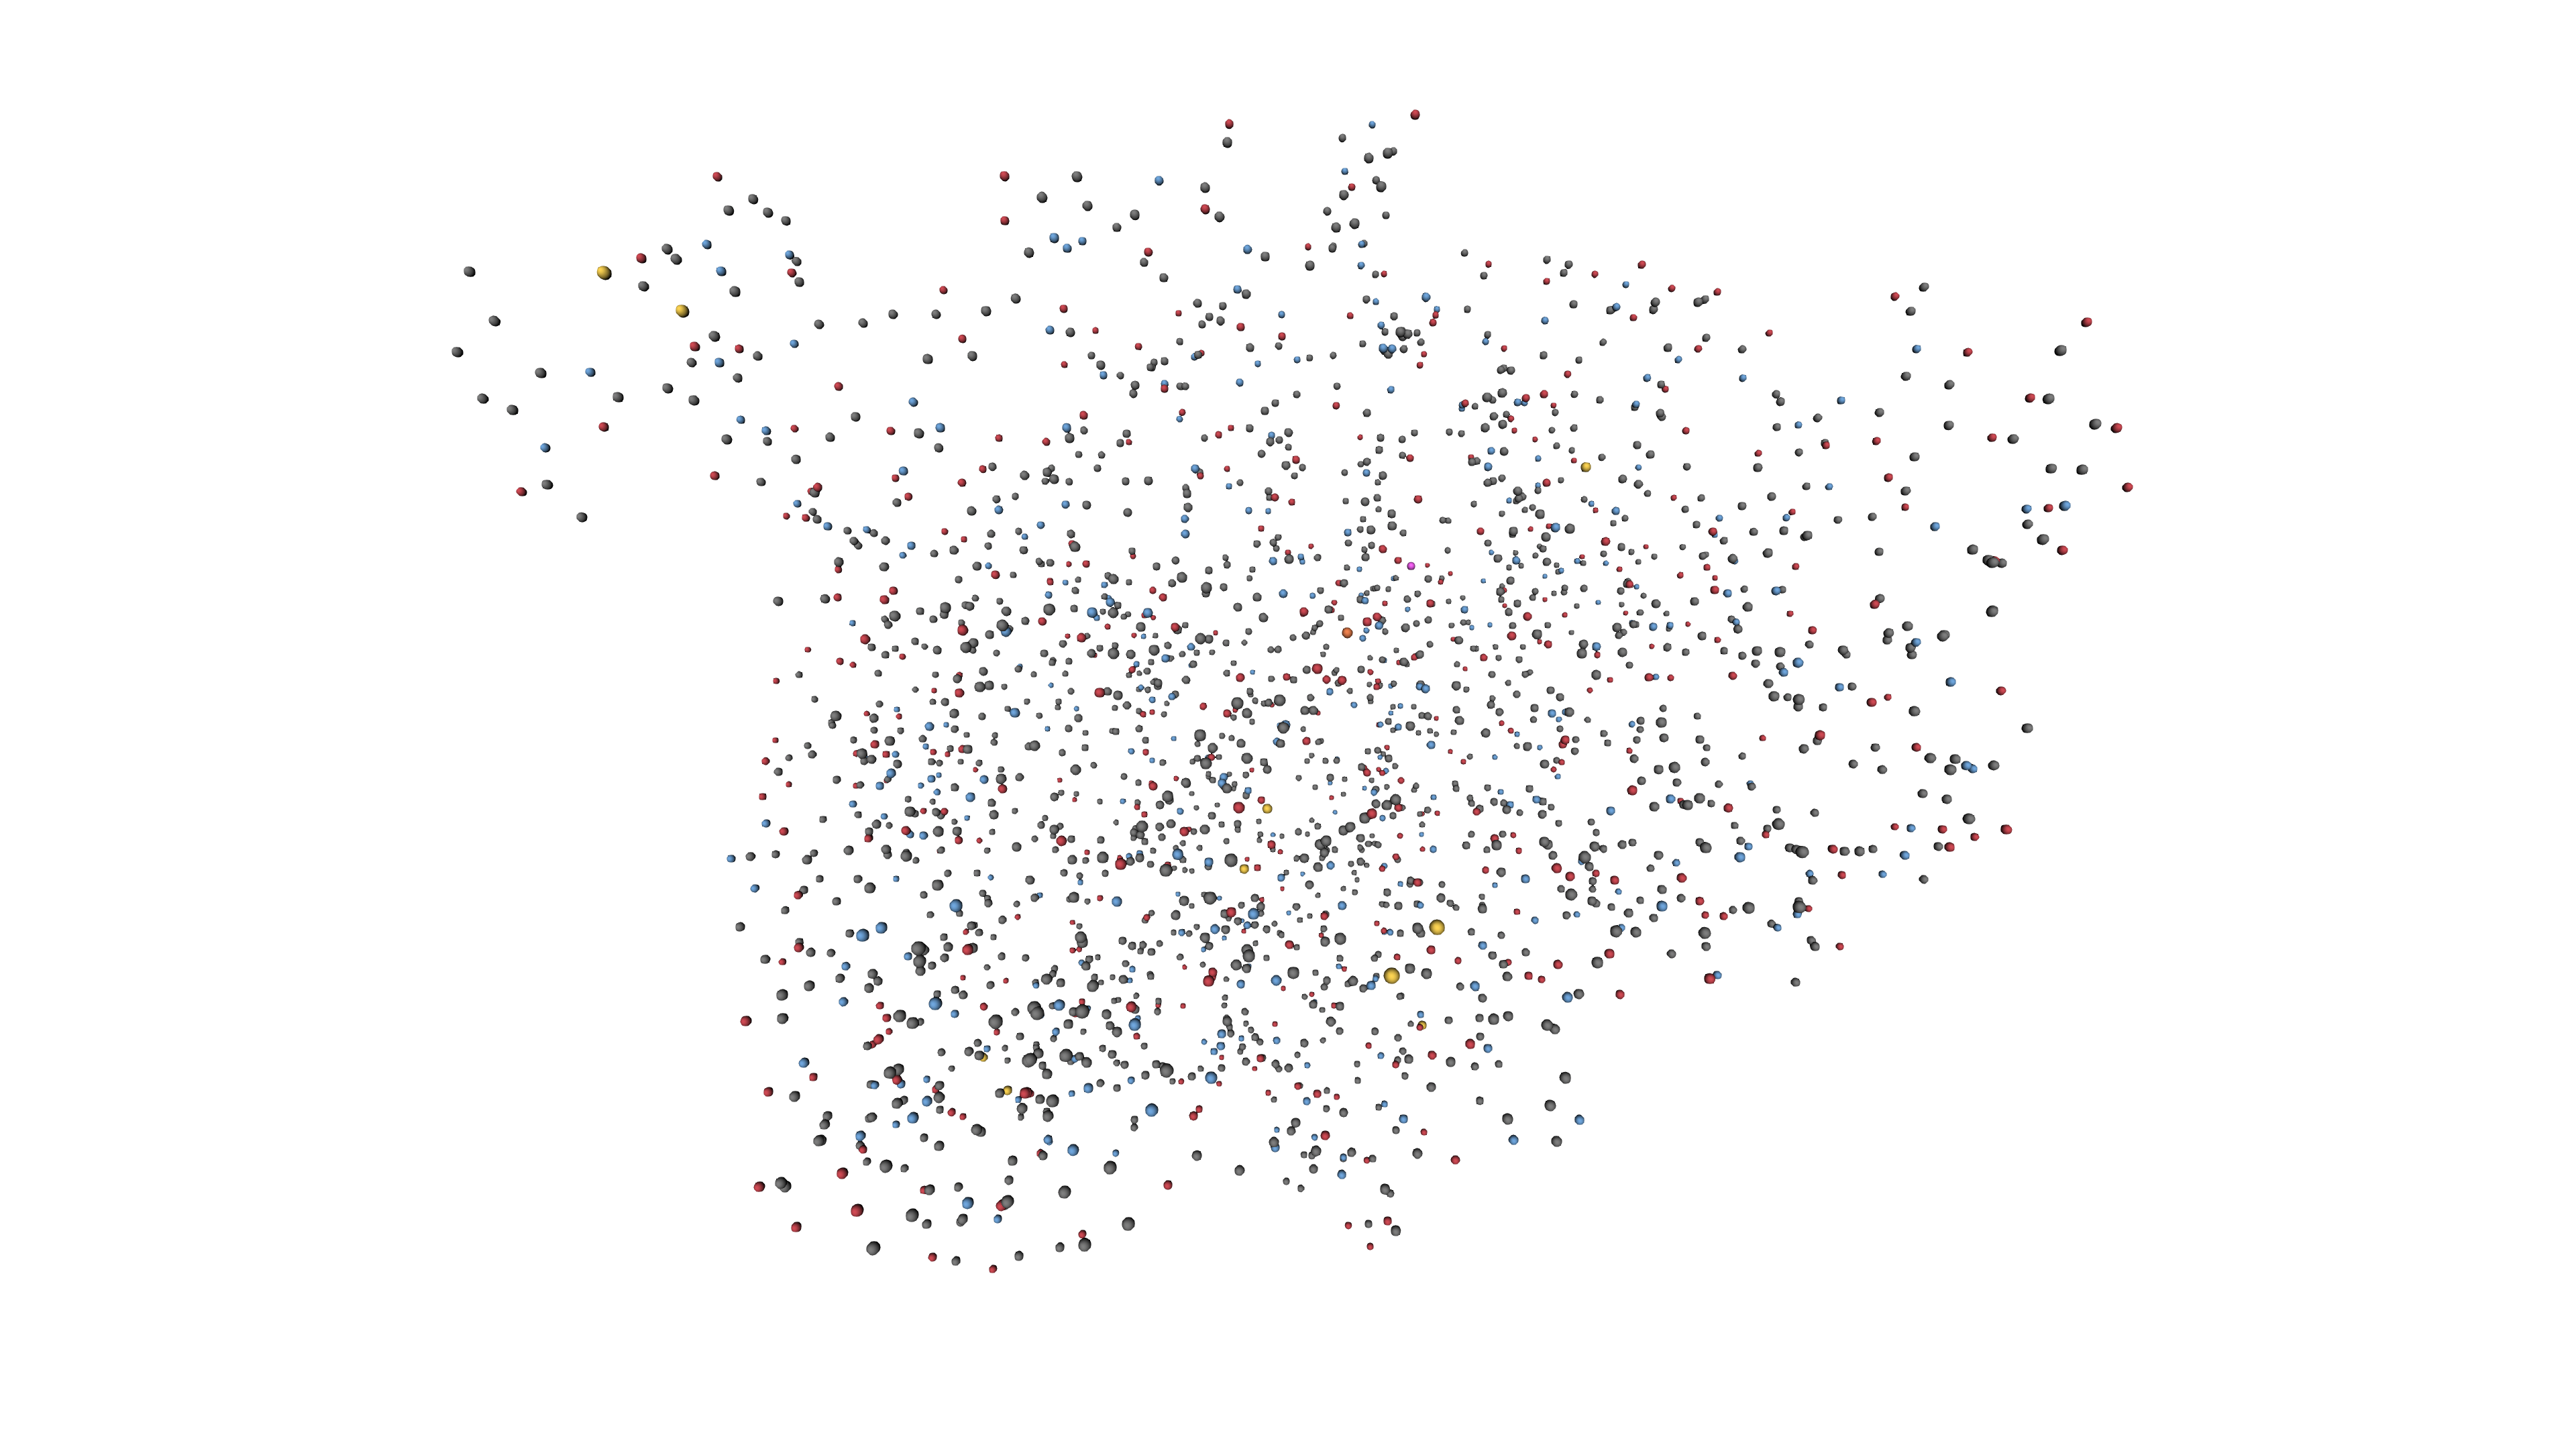
\includegraphics[width=\textwidth]{./figures/ch1/4awn_points}
			\caption[Représentation en points]{\textbf{Points :} seuls les atomes apparaissent.}
			\label{fig:4awn_points}
		\end{subfigure}
		~
		\begin{subfigure}[t]{\subImgW}
			\centering
			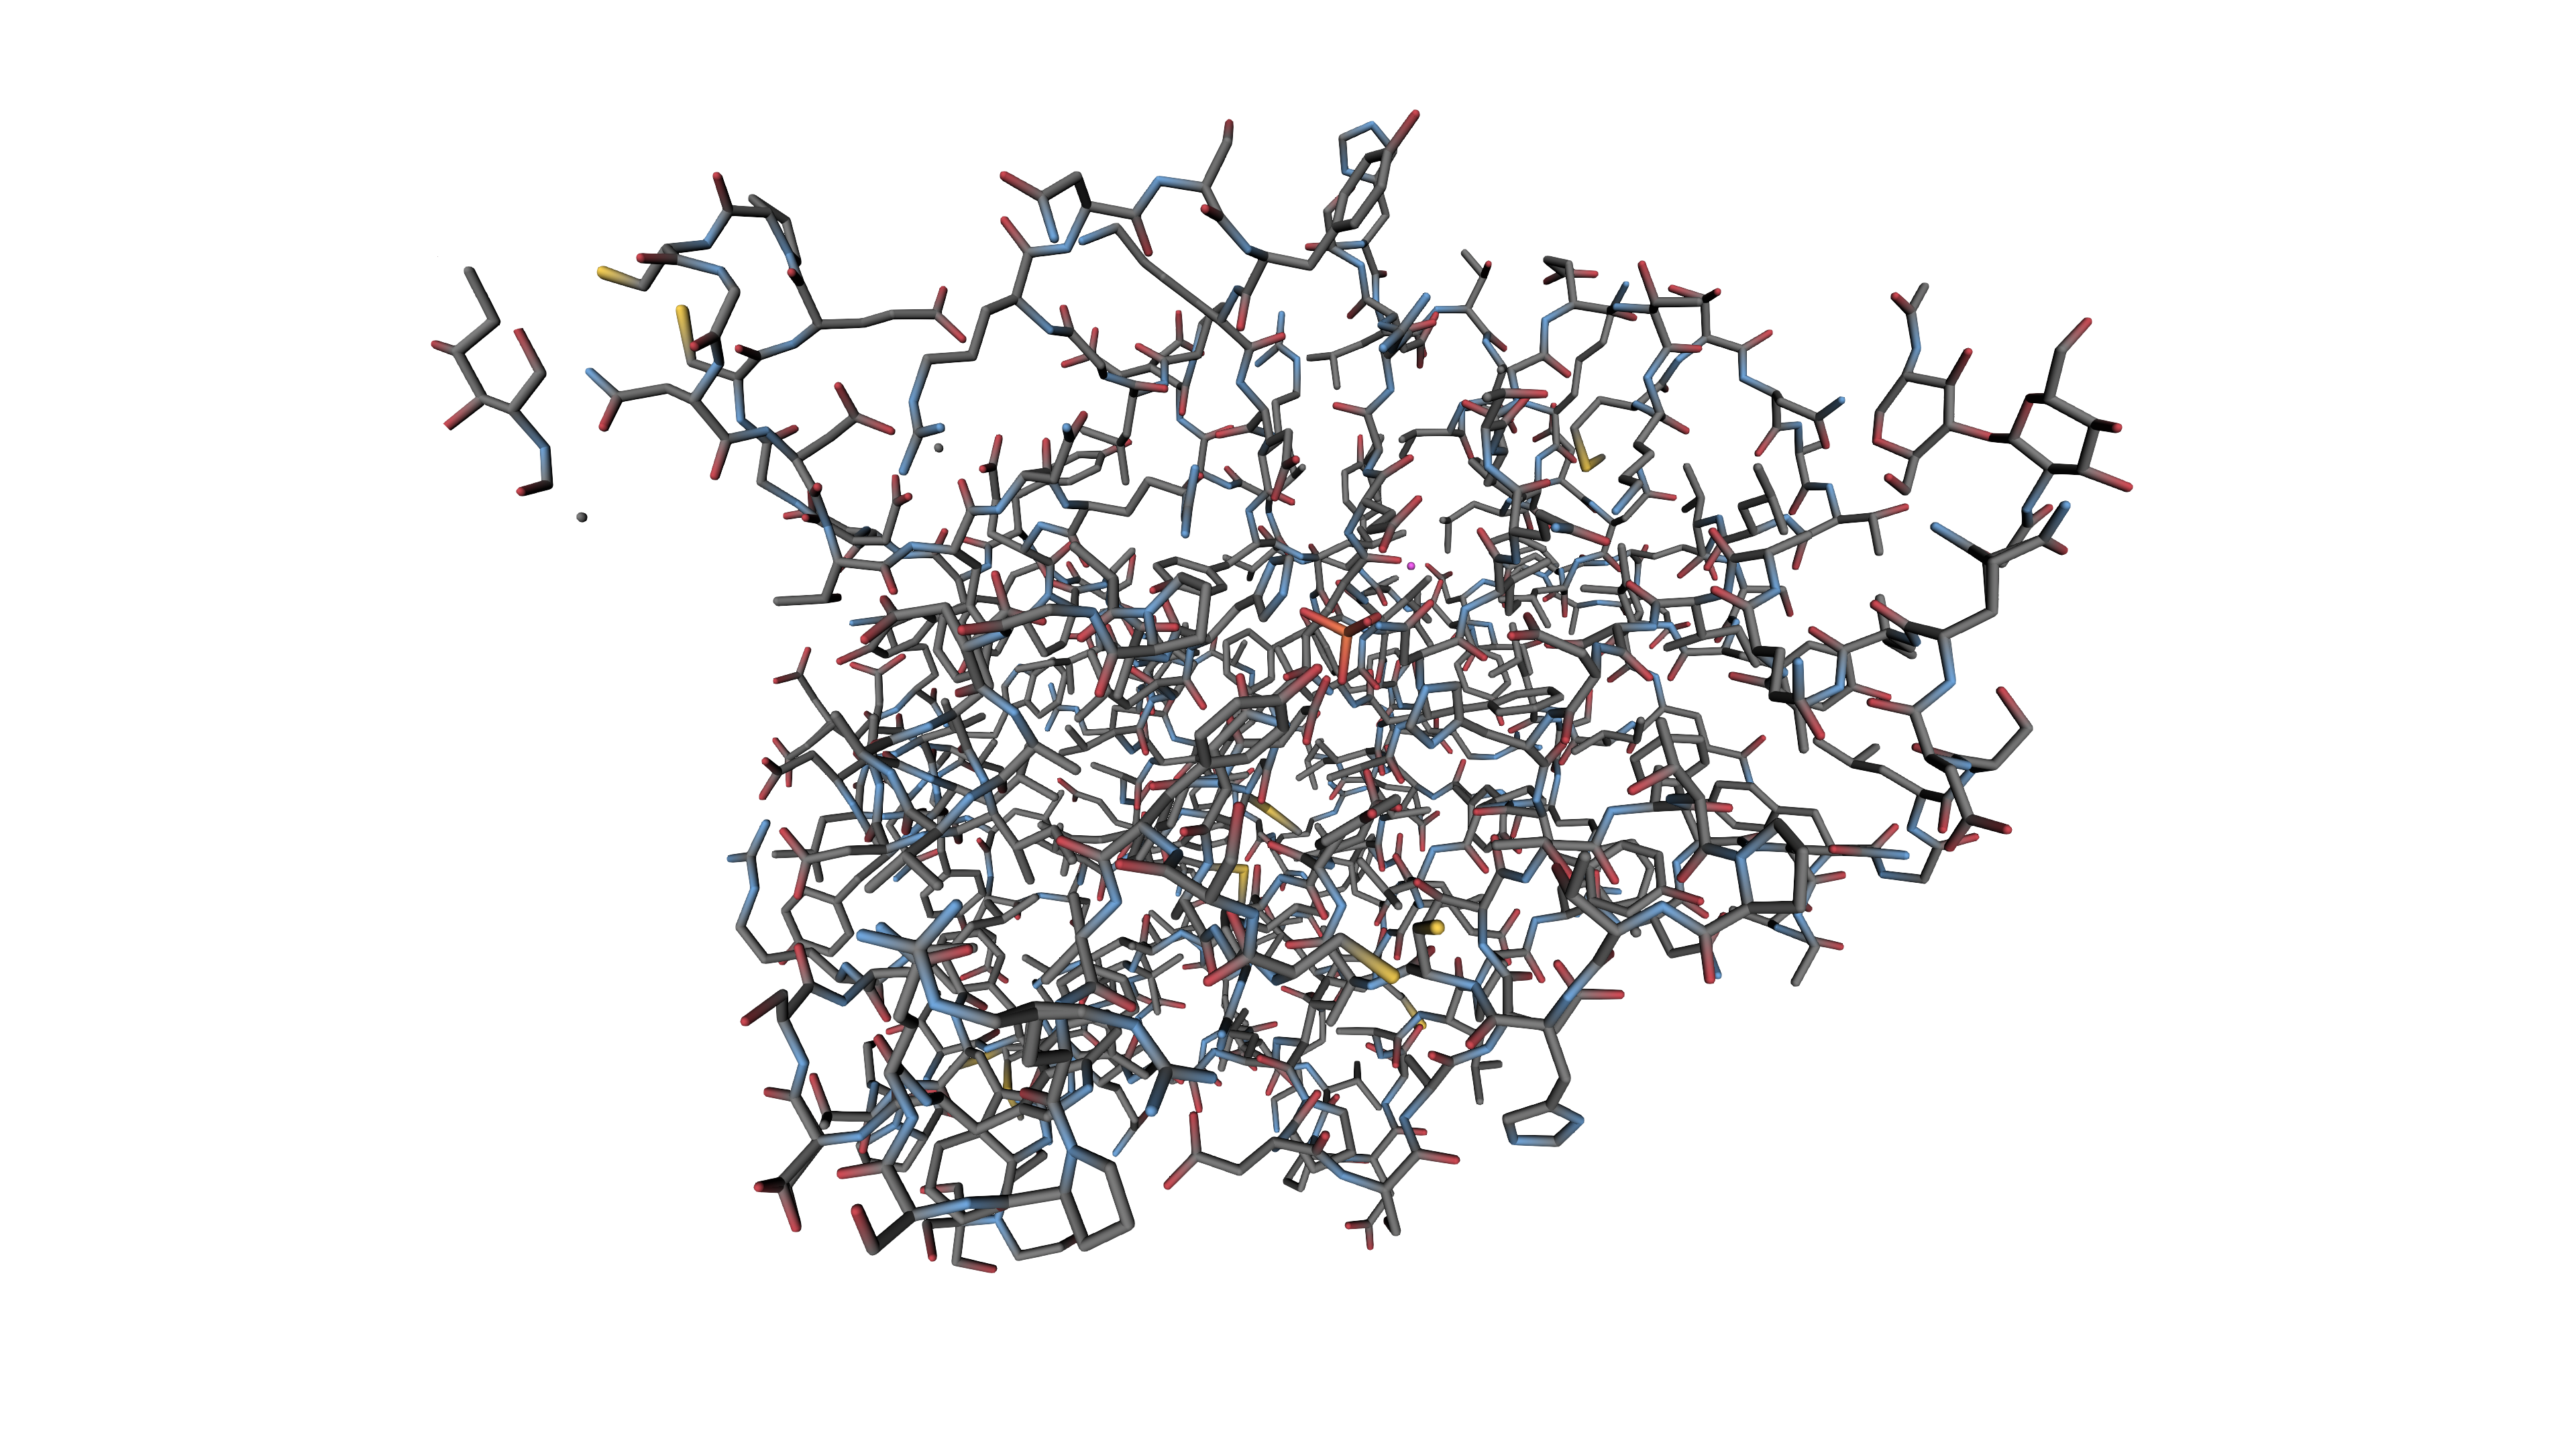
\includegraphics[width=\textwidth]{./figures/ch1/4awn_licorice}
			\caption[Représentation en réglisse]{\textbf{Bâtons, réglisse ou \emph{licorice} :} seules les liaisons covalentes sont visibles.}
			\label{fig:4awn_licorice}
		\end{subfigure}
		~
		\begin{subfigure}[t]{\subImgW}
			\centering
			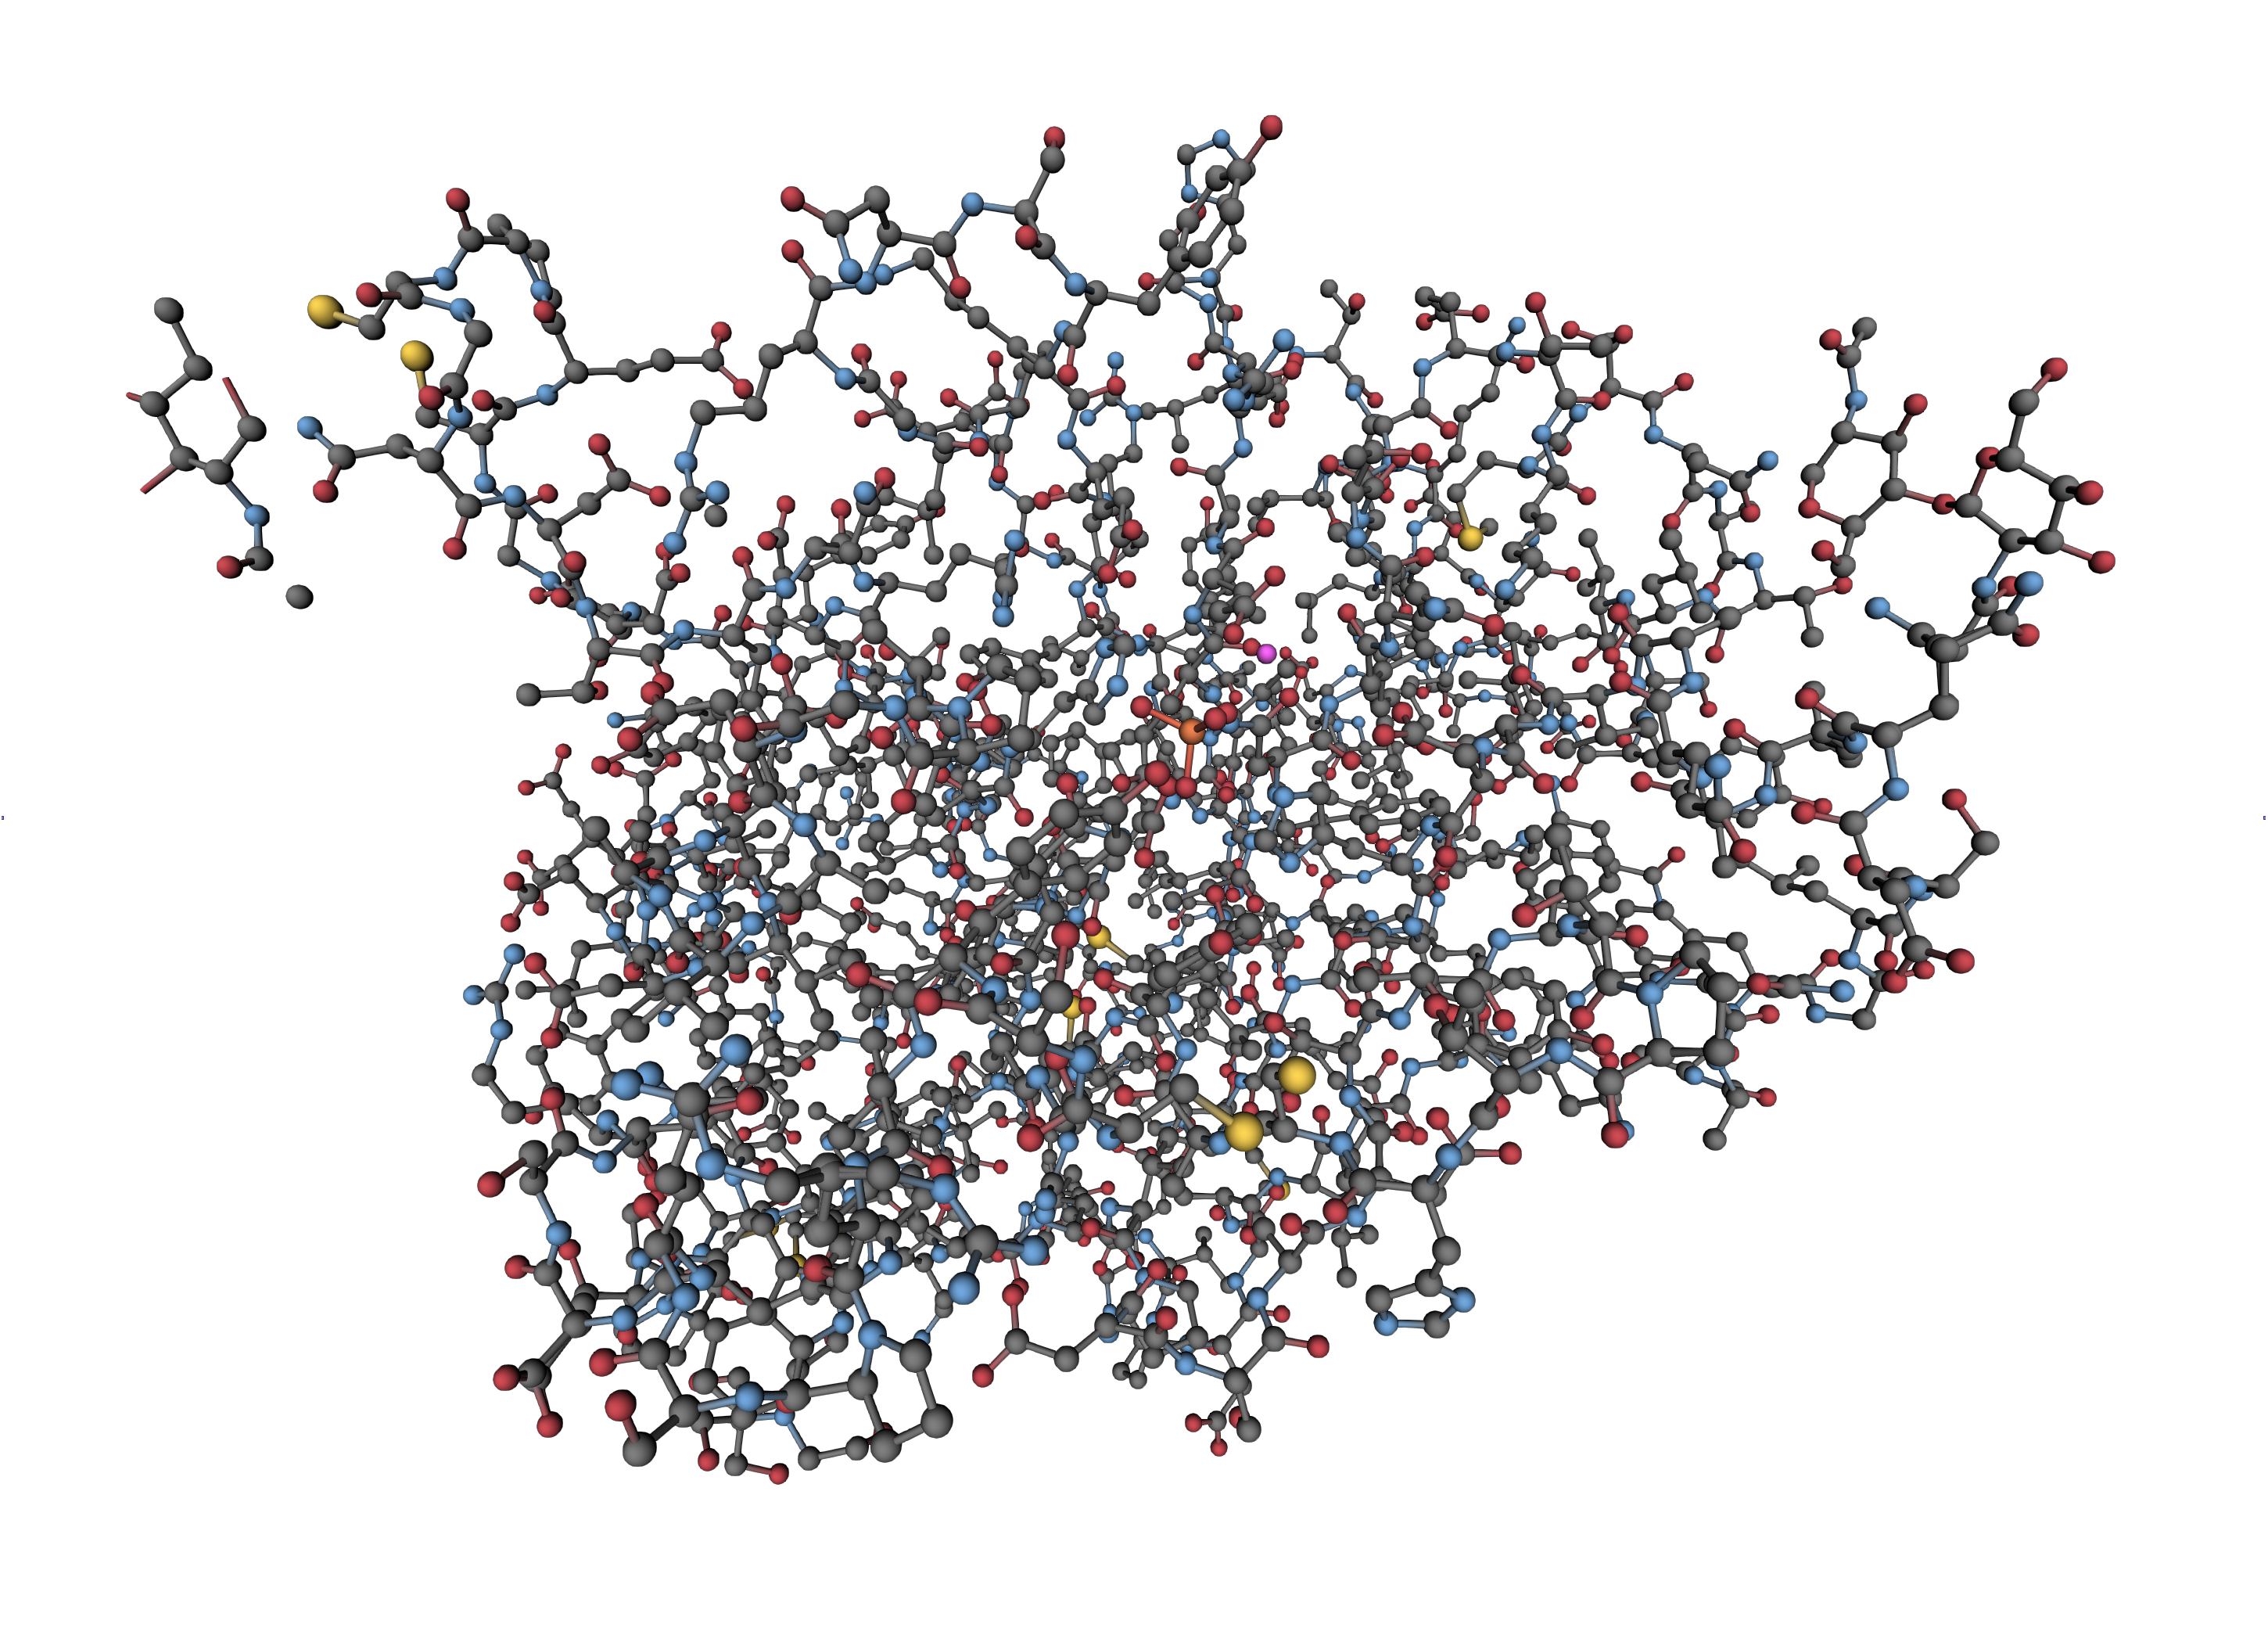
\includegraphics[width=\textwidth]{./figures/ch1/4awn_CPK}
			\caption[Représentation en CPK]{\textbf{CPK/boules et bâtons :} les atomes et les liaisons sont représentés.}
			\label{fig:4awn_CPK}
		\end{subfigure}
		~
		\begin{subfigure}[t]{\subImgW}
			\centering
			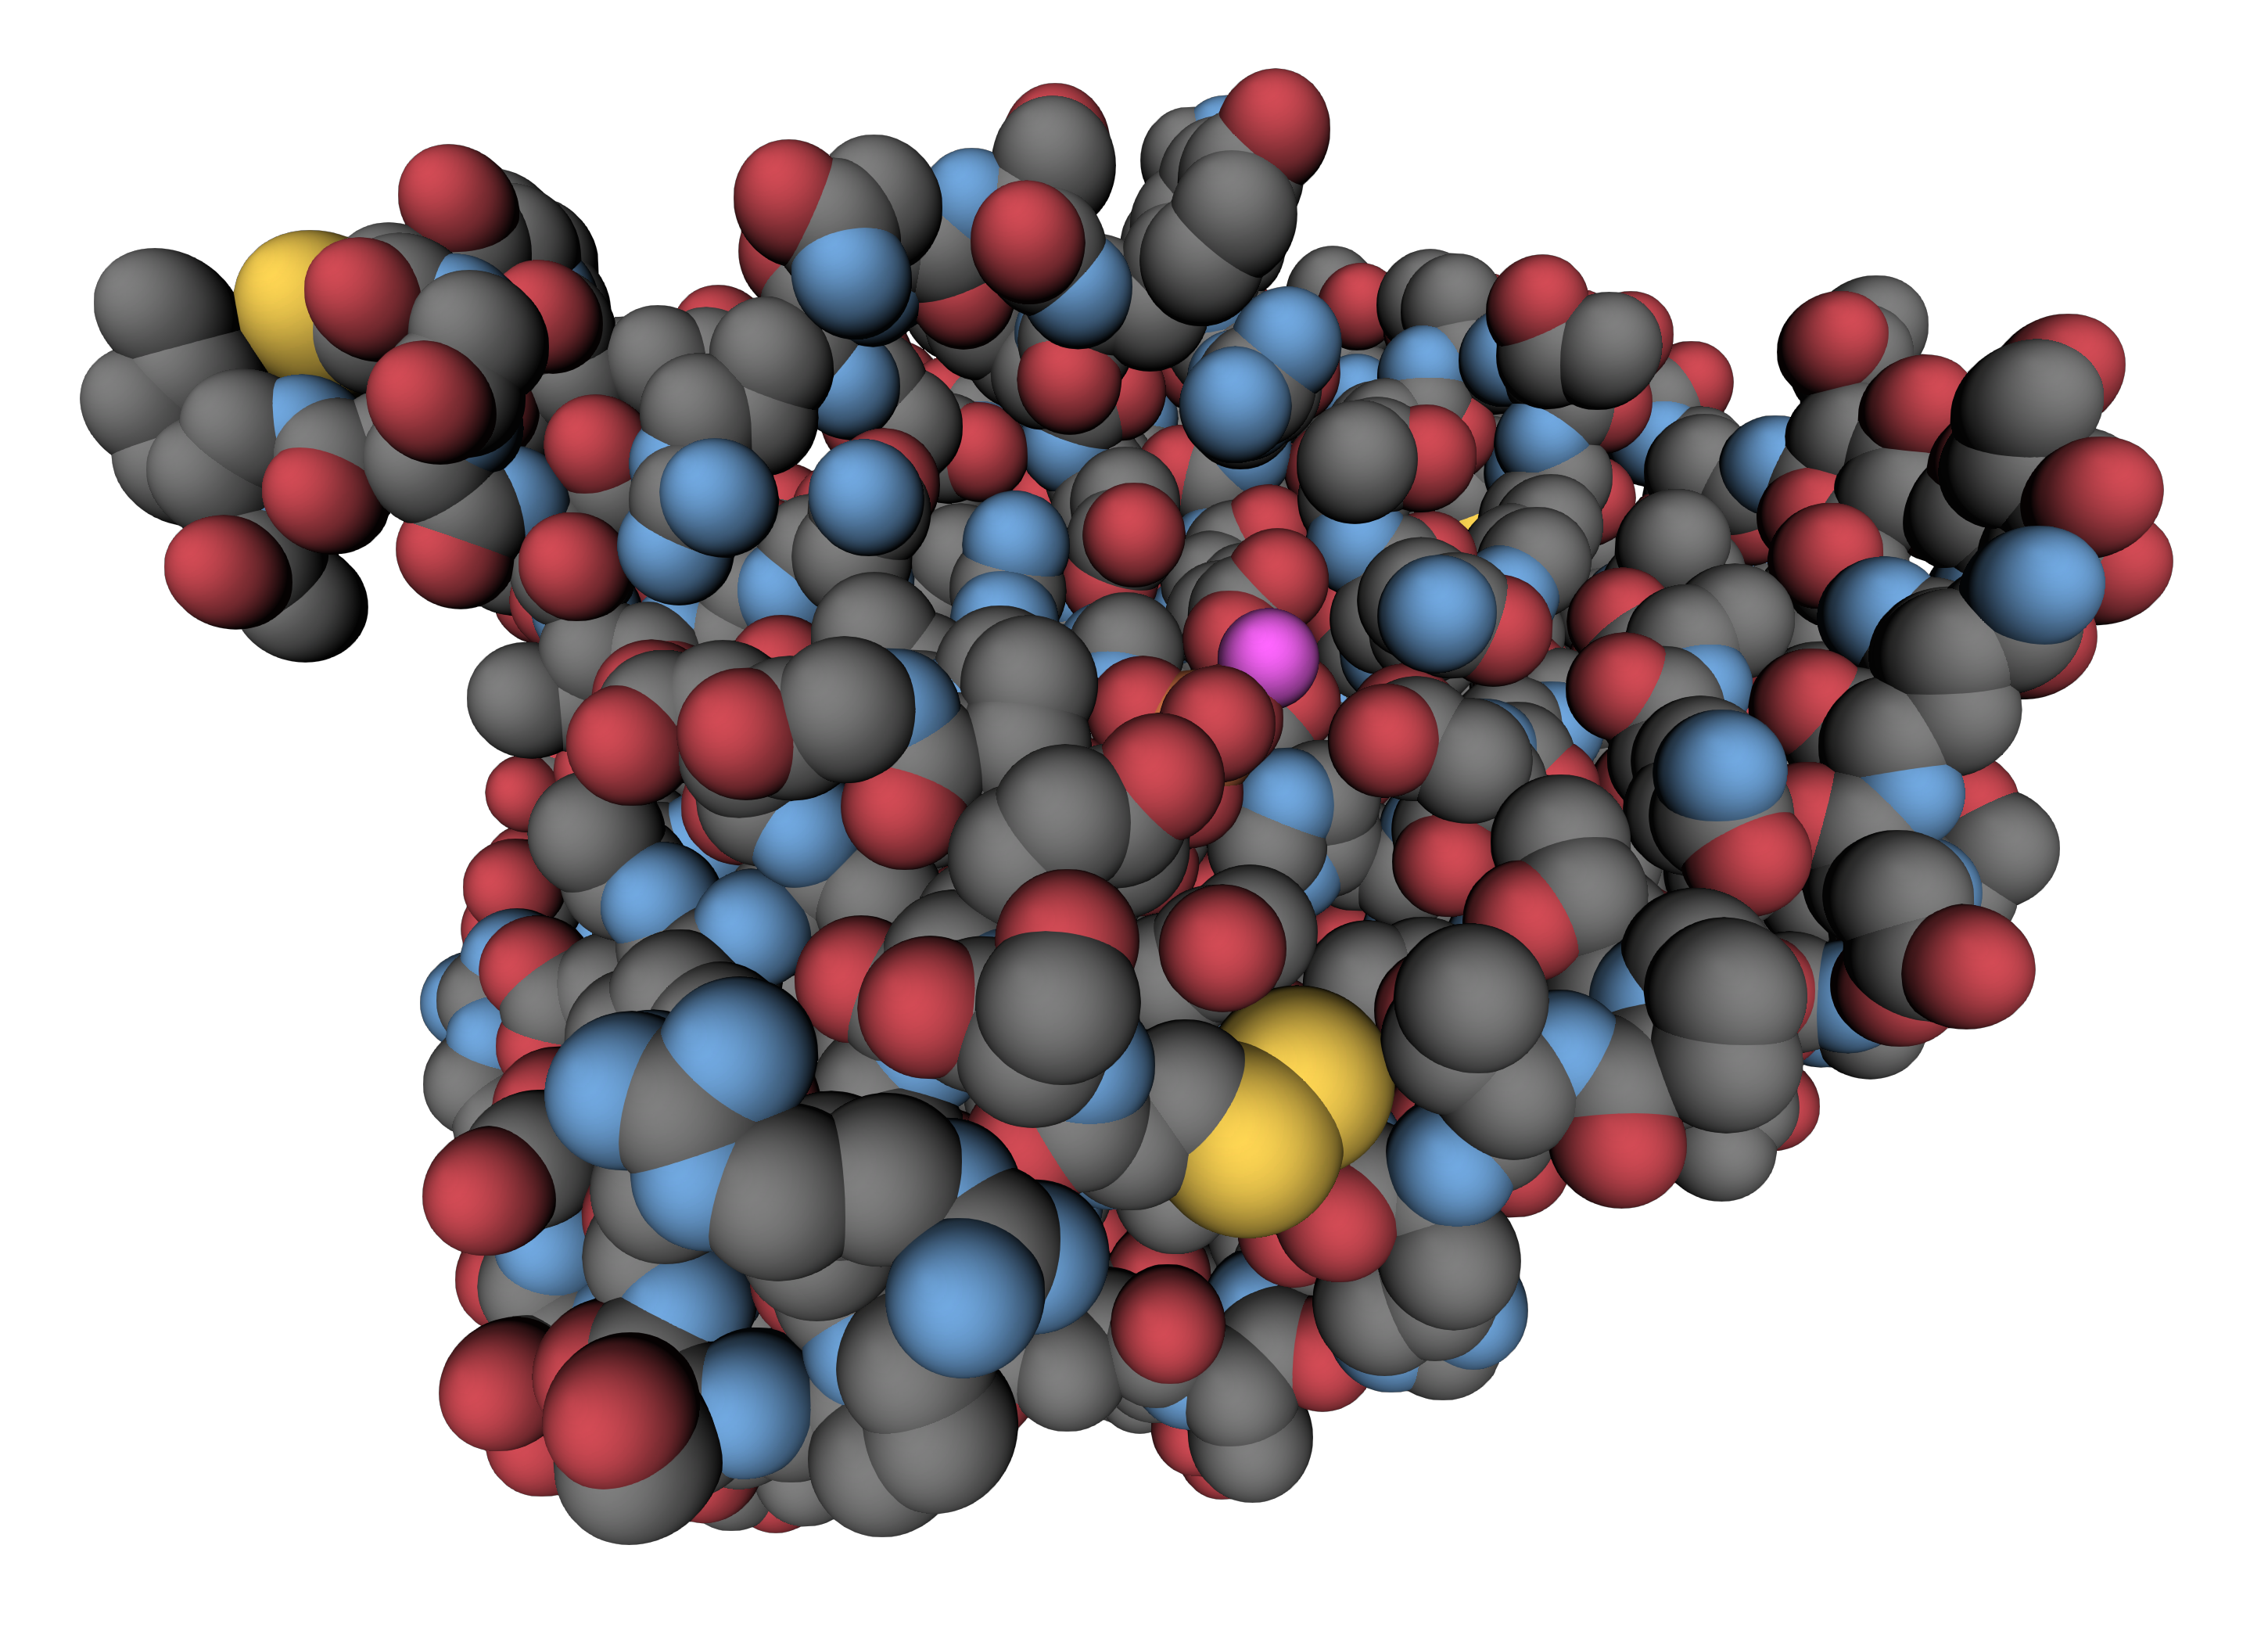
\includegraphics[width=\textwidth]{./figures/ch1/4awn_vdW}
			\caption[Représentation de van der Waals]{\textbf{Van der Waals :} seuls les atomes sont visibles.}
			\label{fig:4awn_VdW}
		\end{subfigure}
		~
		\begin{subfigure}[t]{\subImgW}
			\centering
			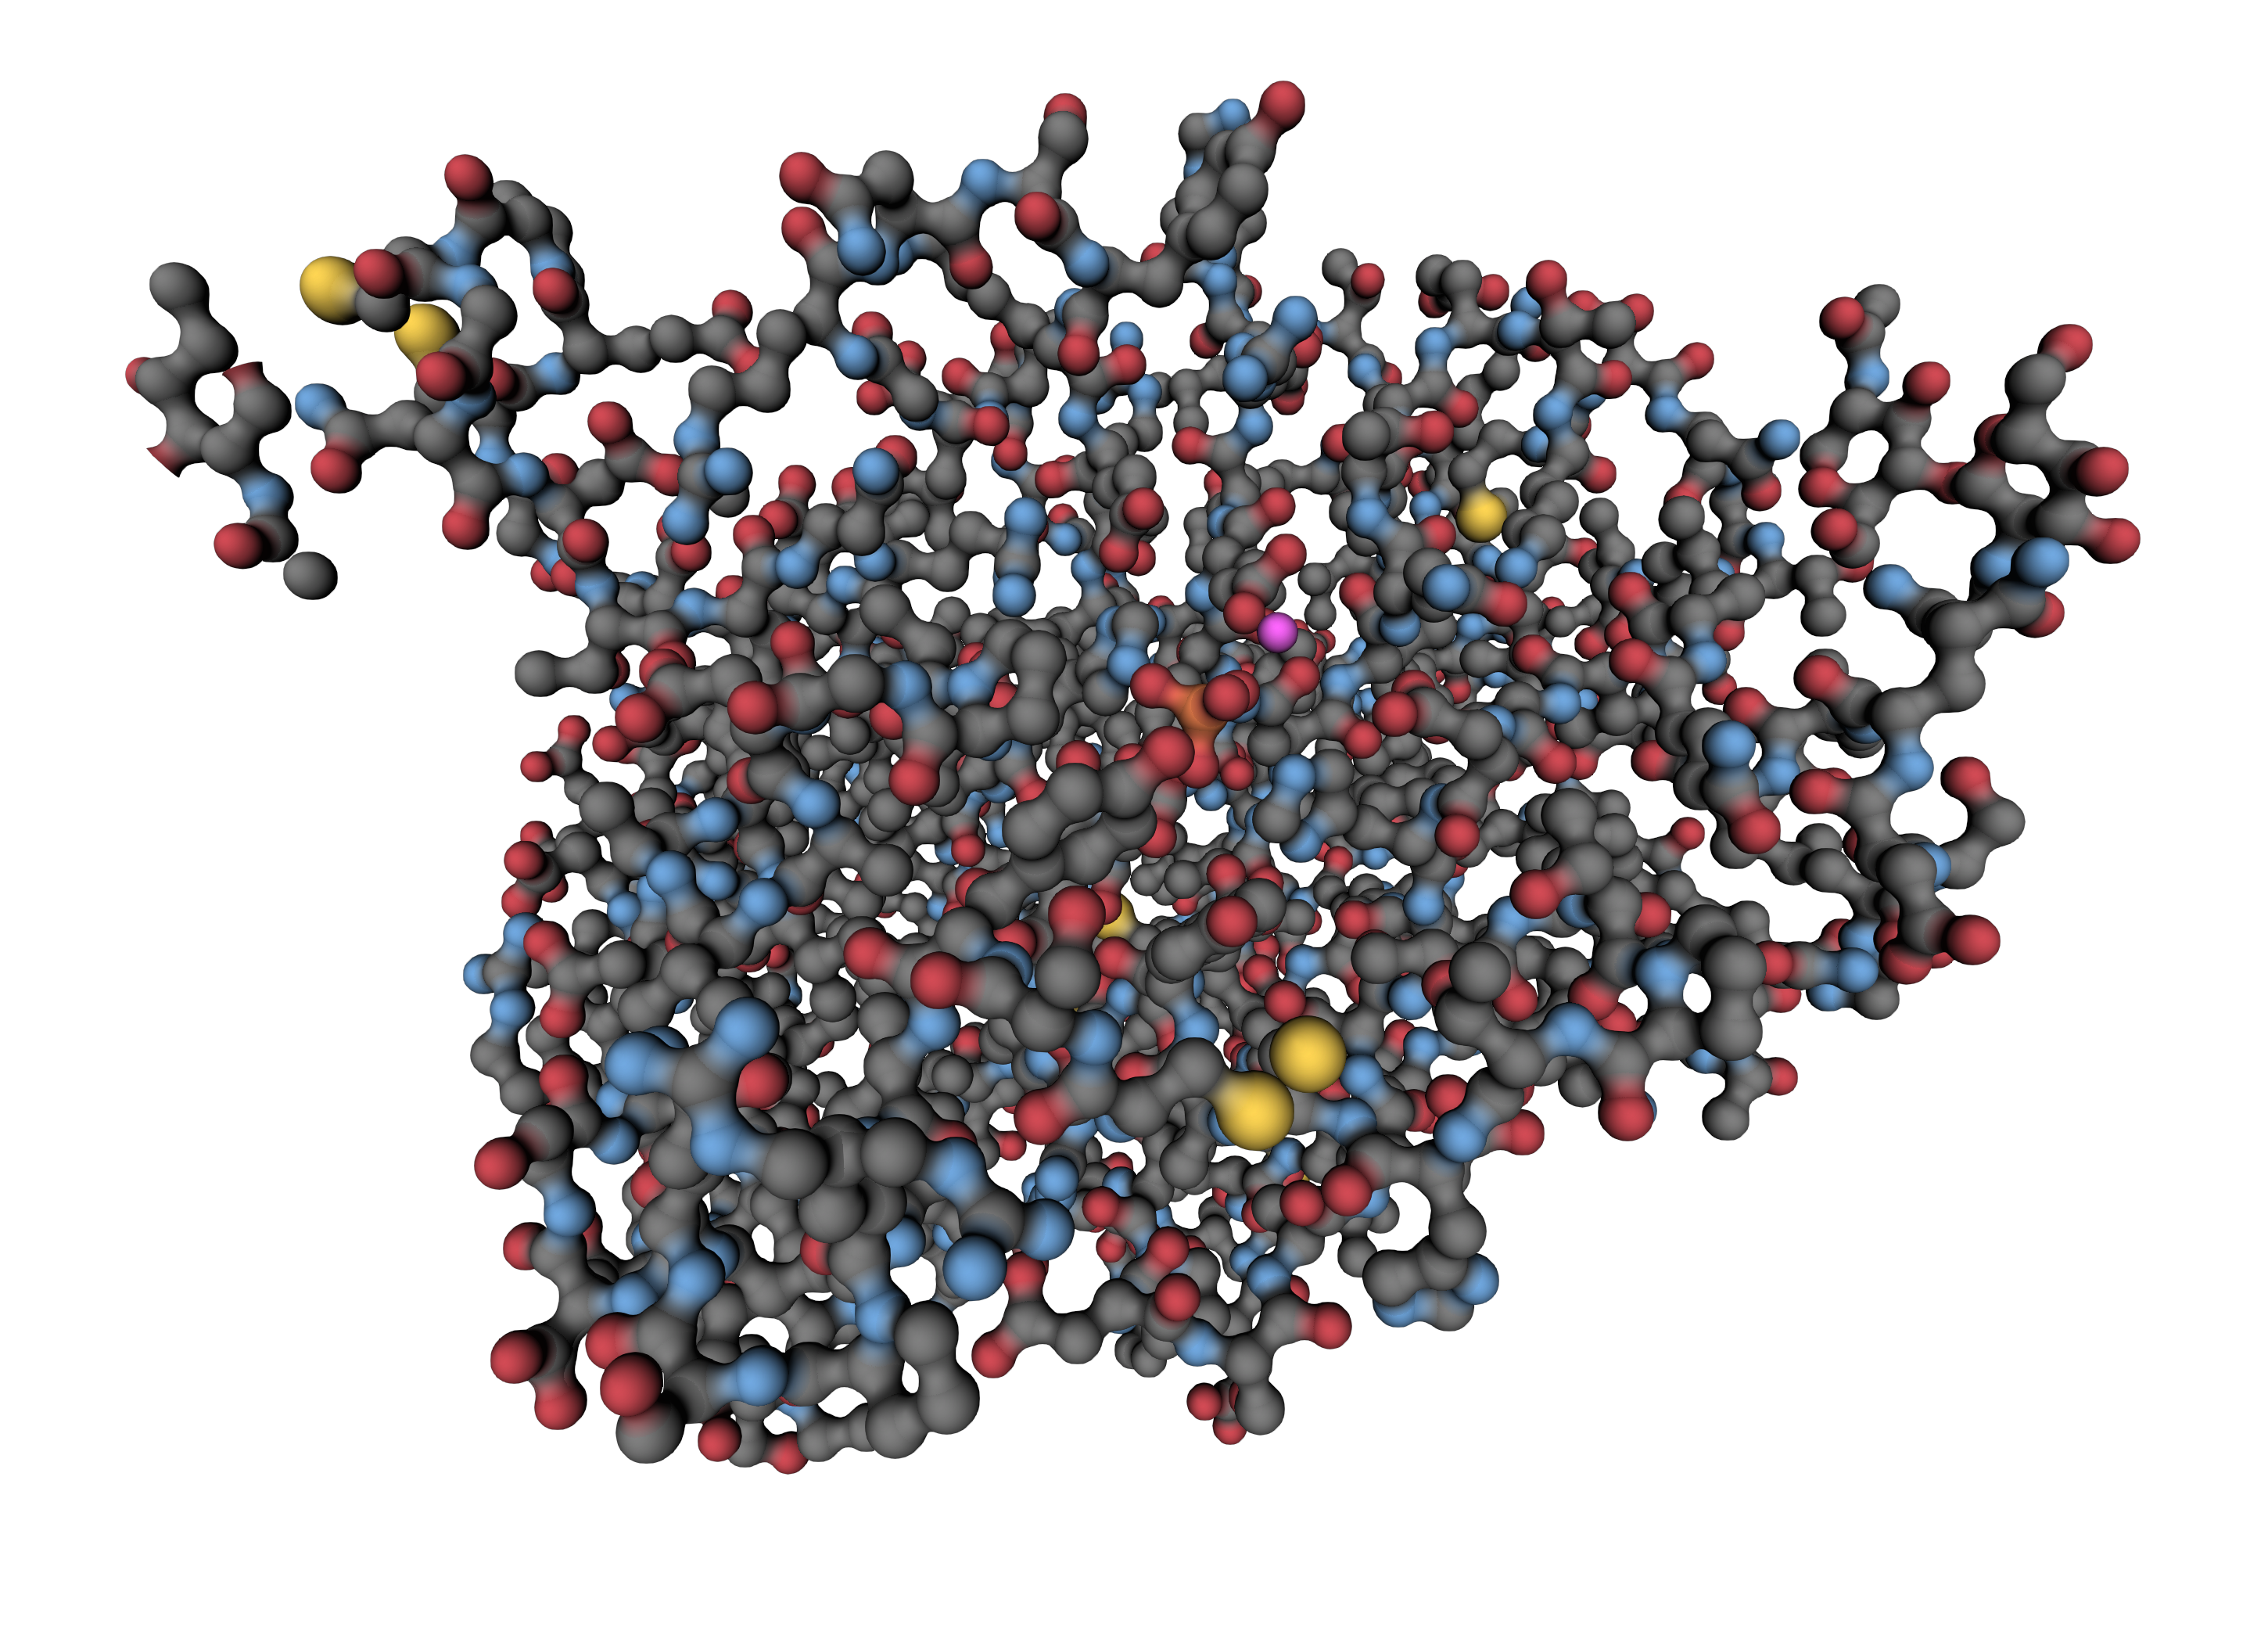
\includegraphics[width=\textwidth]{./figures/ch1/4awn_HB}
			\caption[Représentation en \emph{Hyperballs}]{\textbf{Hyperballs :} les atomes et les liaisons sont représentés~\cite{chavent2011gpu}.}
			\label{fig:4awn_HB}
		\end{subfigure}
		~
		\begin{subfigure}[t]{\subImgW}
			\centering
			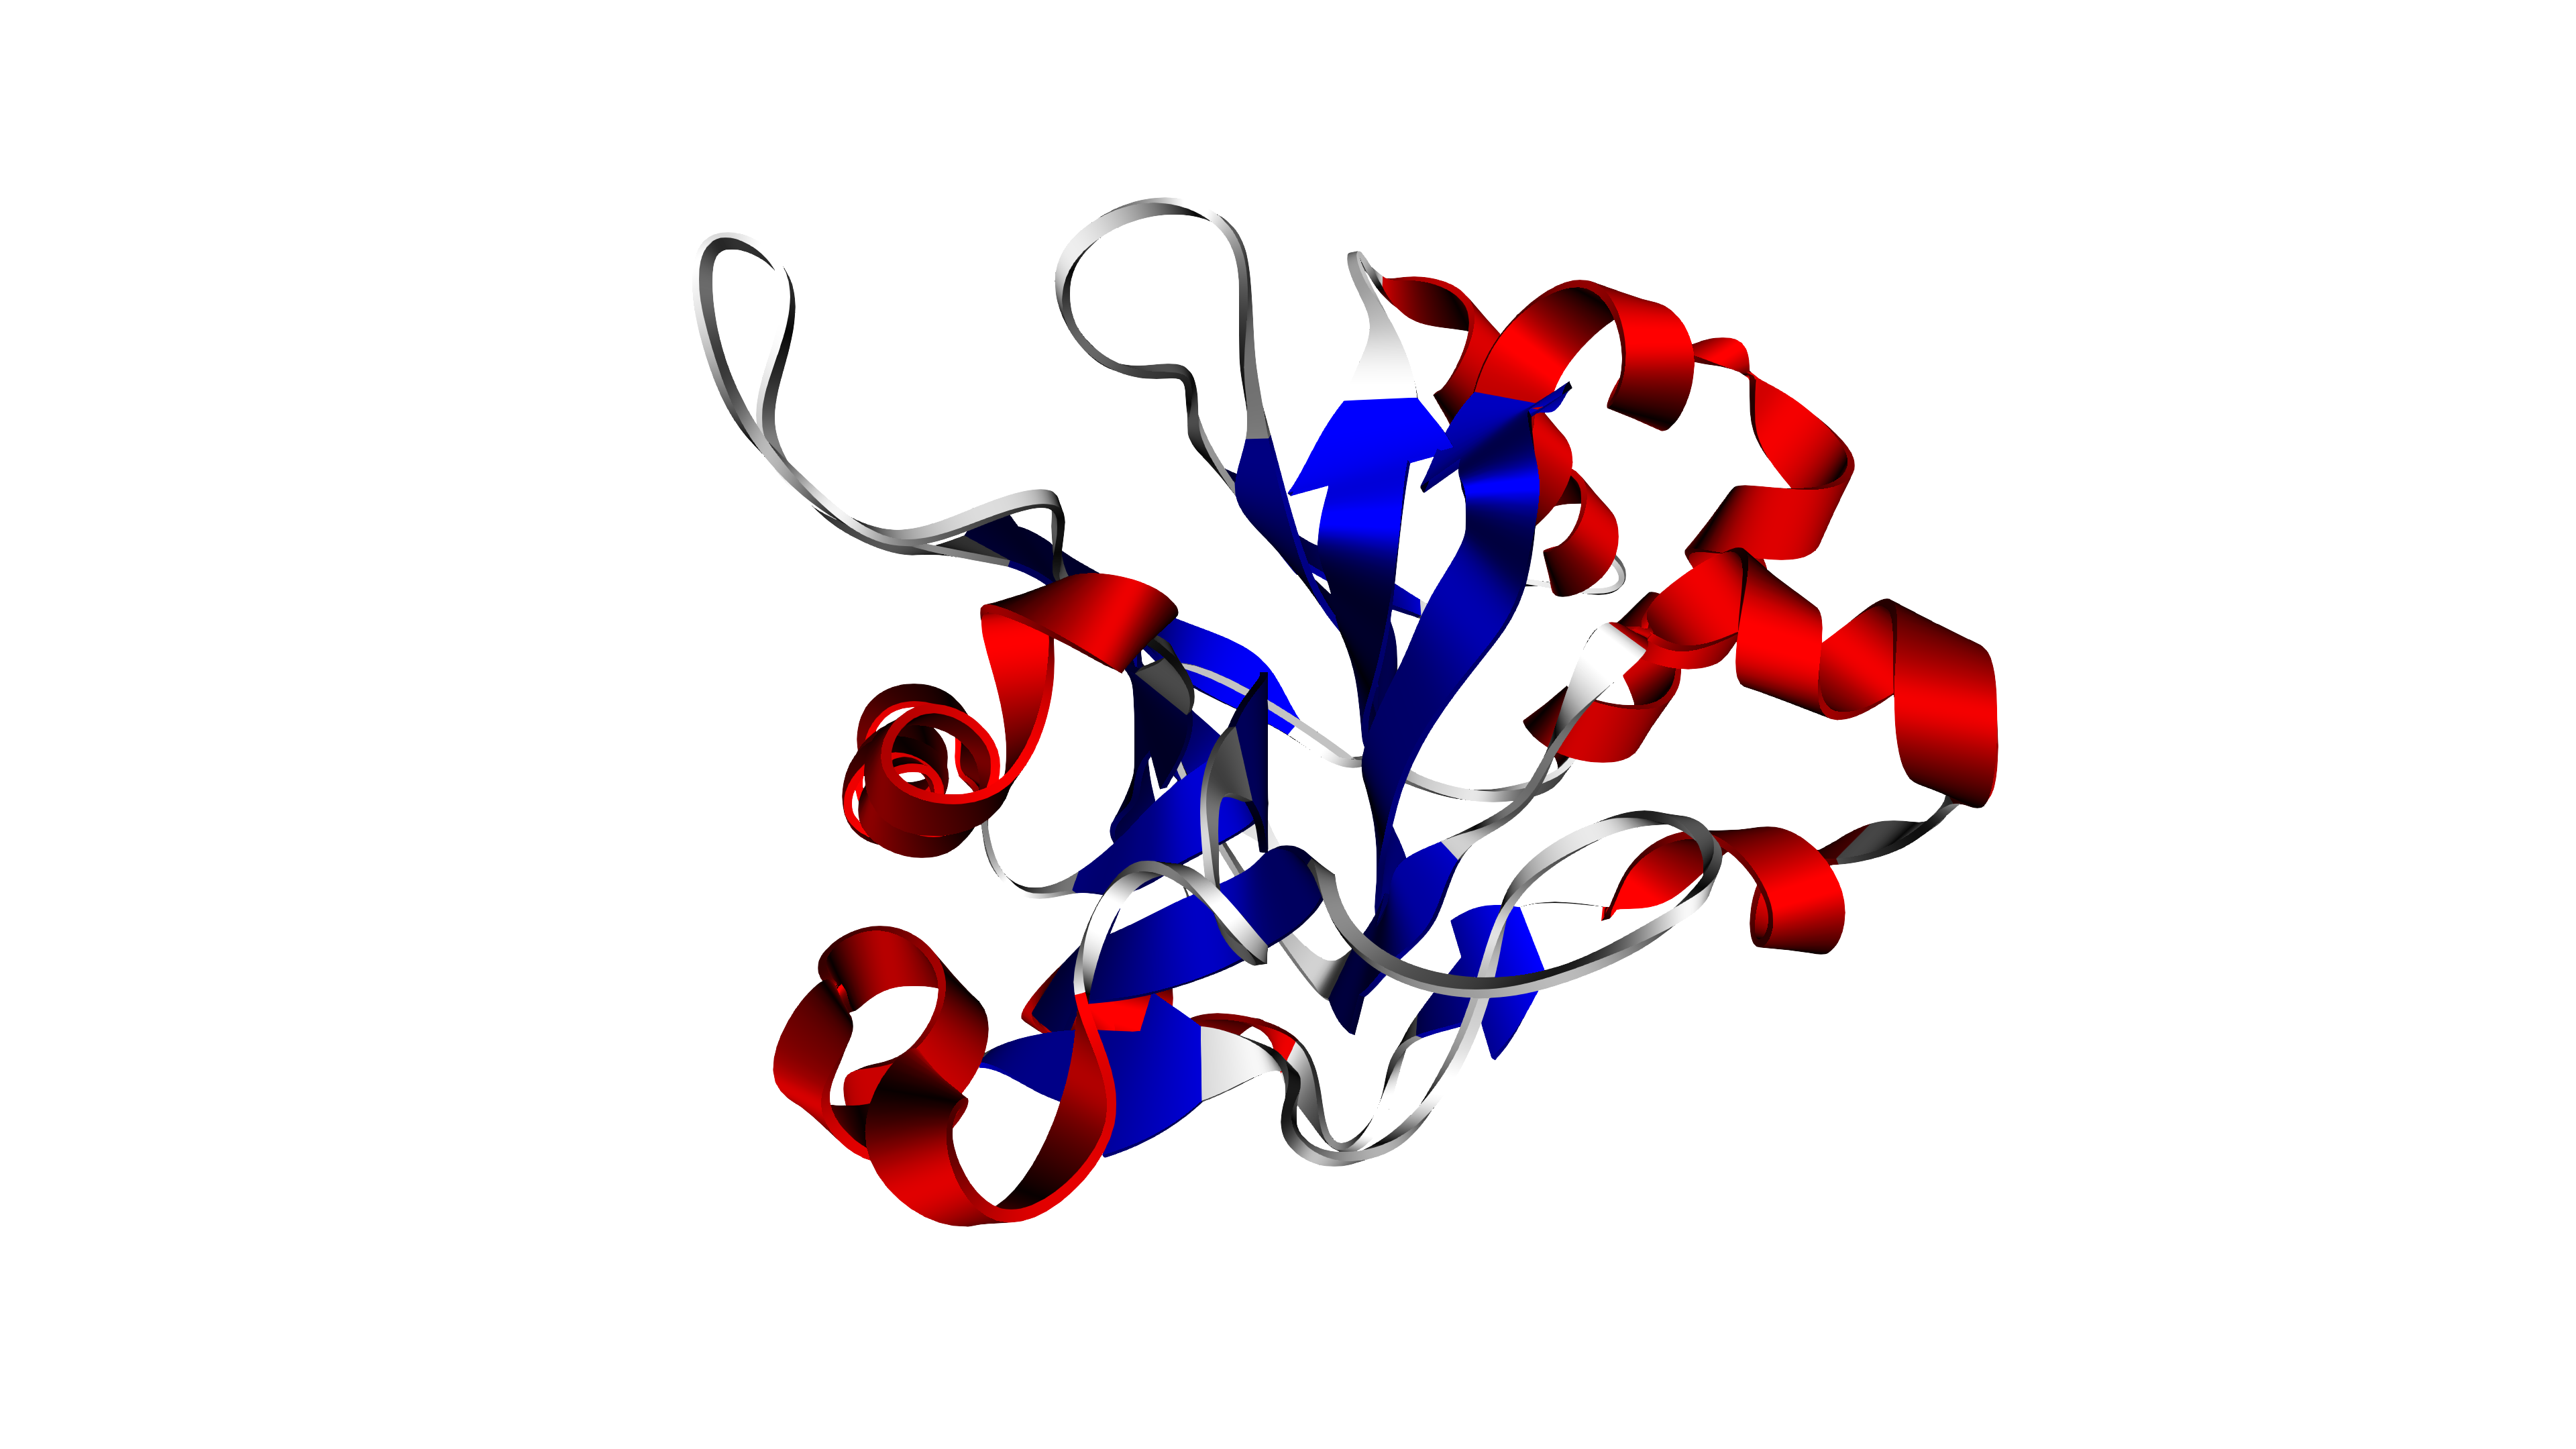
\includegraphics[width=\textwidth]{./figures/ch1/4awn_ss}
			\caption[Représentation en structures secondaires]{\textbf{Structures secondaires :} les atomes et les liaisons sont invisibles, mais des structures plus grandes sont représentées de façon schématique.}
			\label{fig:4awn_ss}
		\end{subfigure}
		~
		\begin{subfigure}[t]{\subImgW}
			\centering
			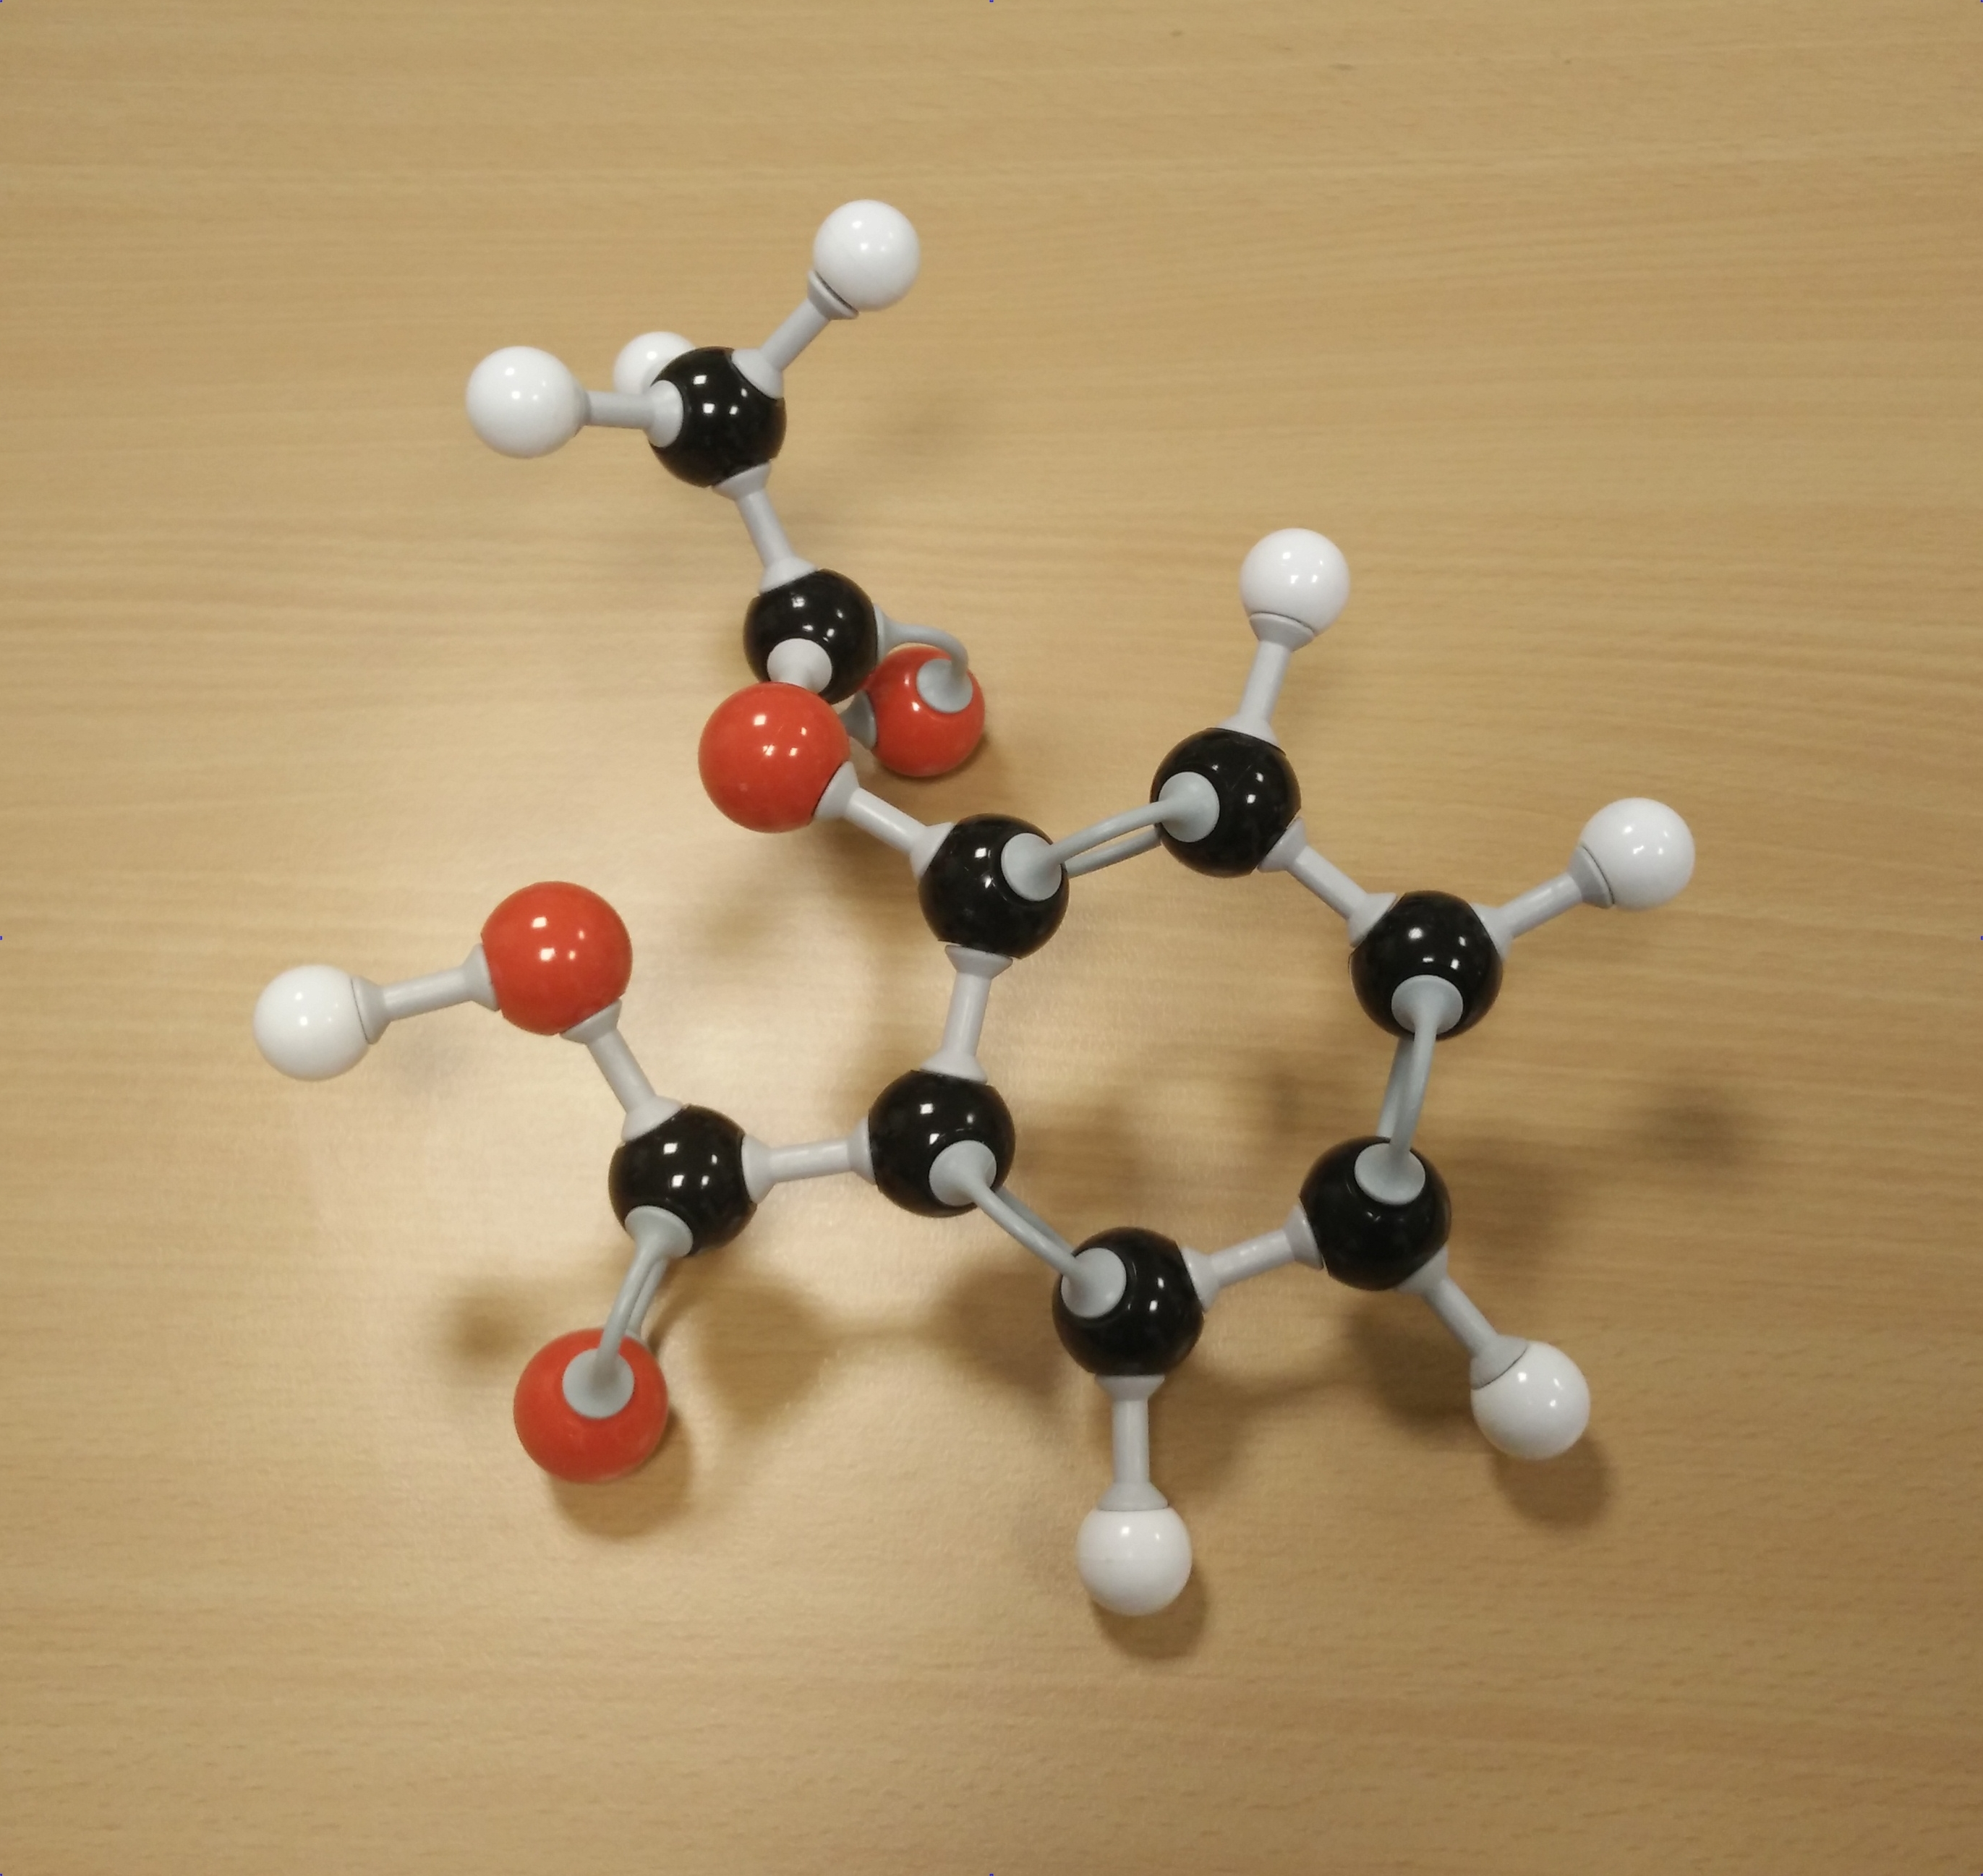
\includegraphics[width=\textwidth]{./figures/ch1/aspirin}
			\caption[Modèle physique de l'aspirine]{\textbf{Modèle physique }d'aspirine (et non d'ADNase). Les liaisons doubles sont modélisées par des paires de bâtons pour empêcher les rotations.}
			\label{fig:aspirin}
		\end{subfigure}
		~
		\begin{subfigure}[t]{\subImgW}
			\centering
			\includegraphics[width=\textwidth]{./figures/ch1/4awn_ses}
			\caption[Représentation en surface de Connolly]{\textbf{Surface de Connolly, ou \emph{solvent excluded surface} :} les points de contact entre une molécule d'eau et l'ADNase.}
			\label{fig:4awn_ses}
		\end{subfigure}
		~
		\begin{subfigure}[t]{\subImgW}
			\centering
			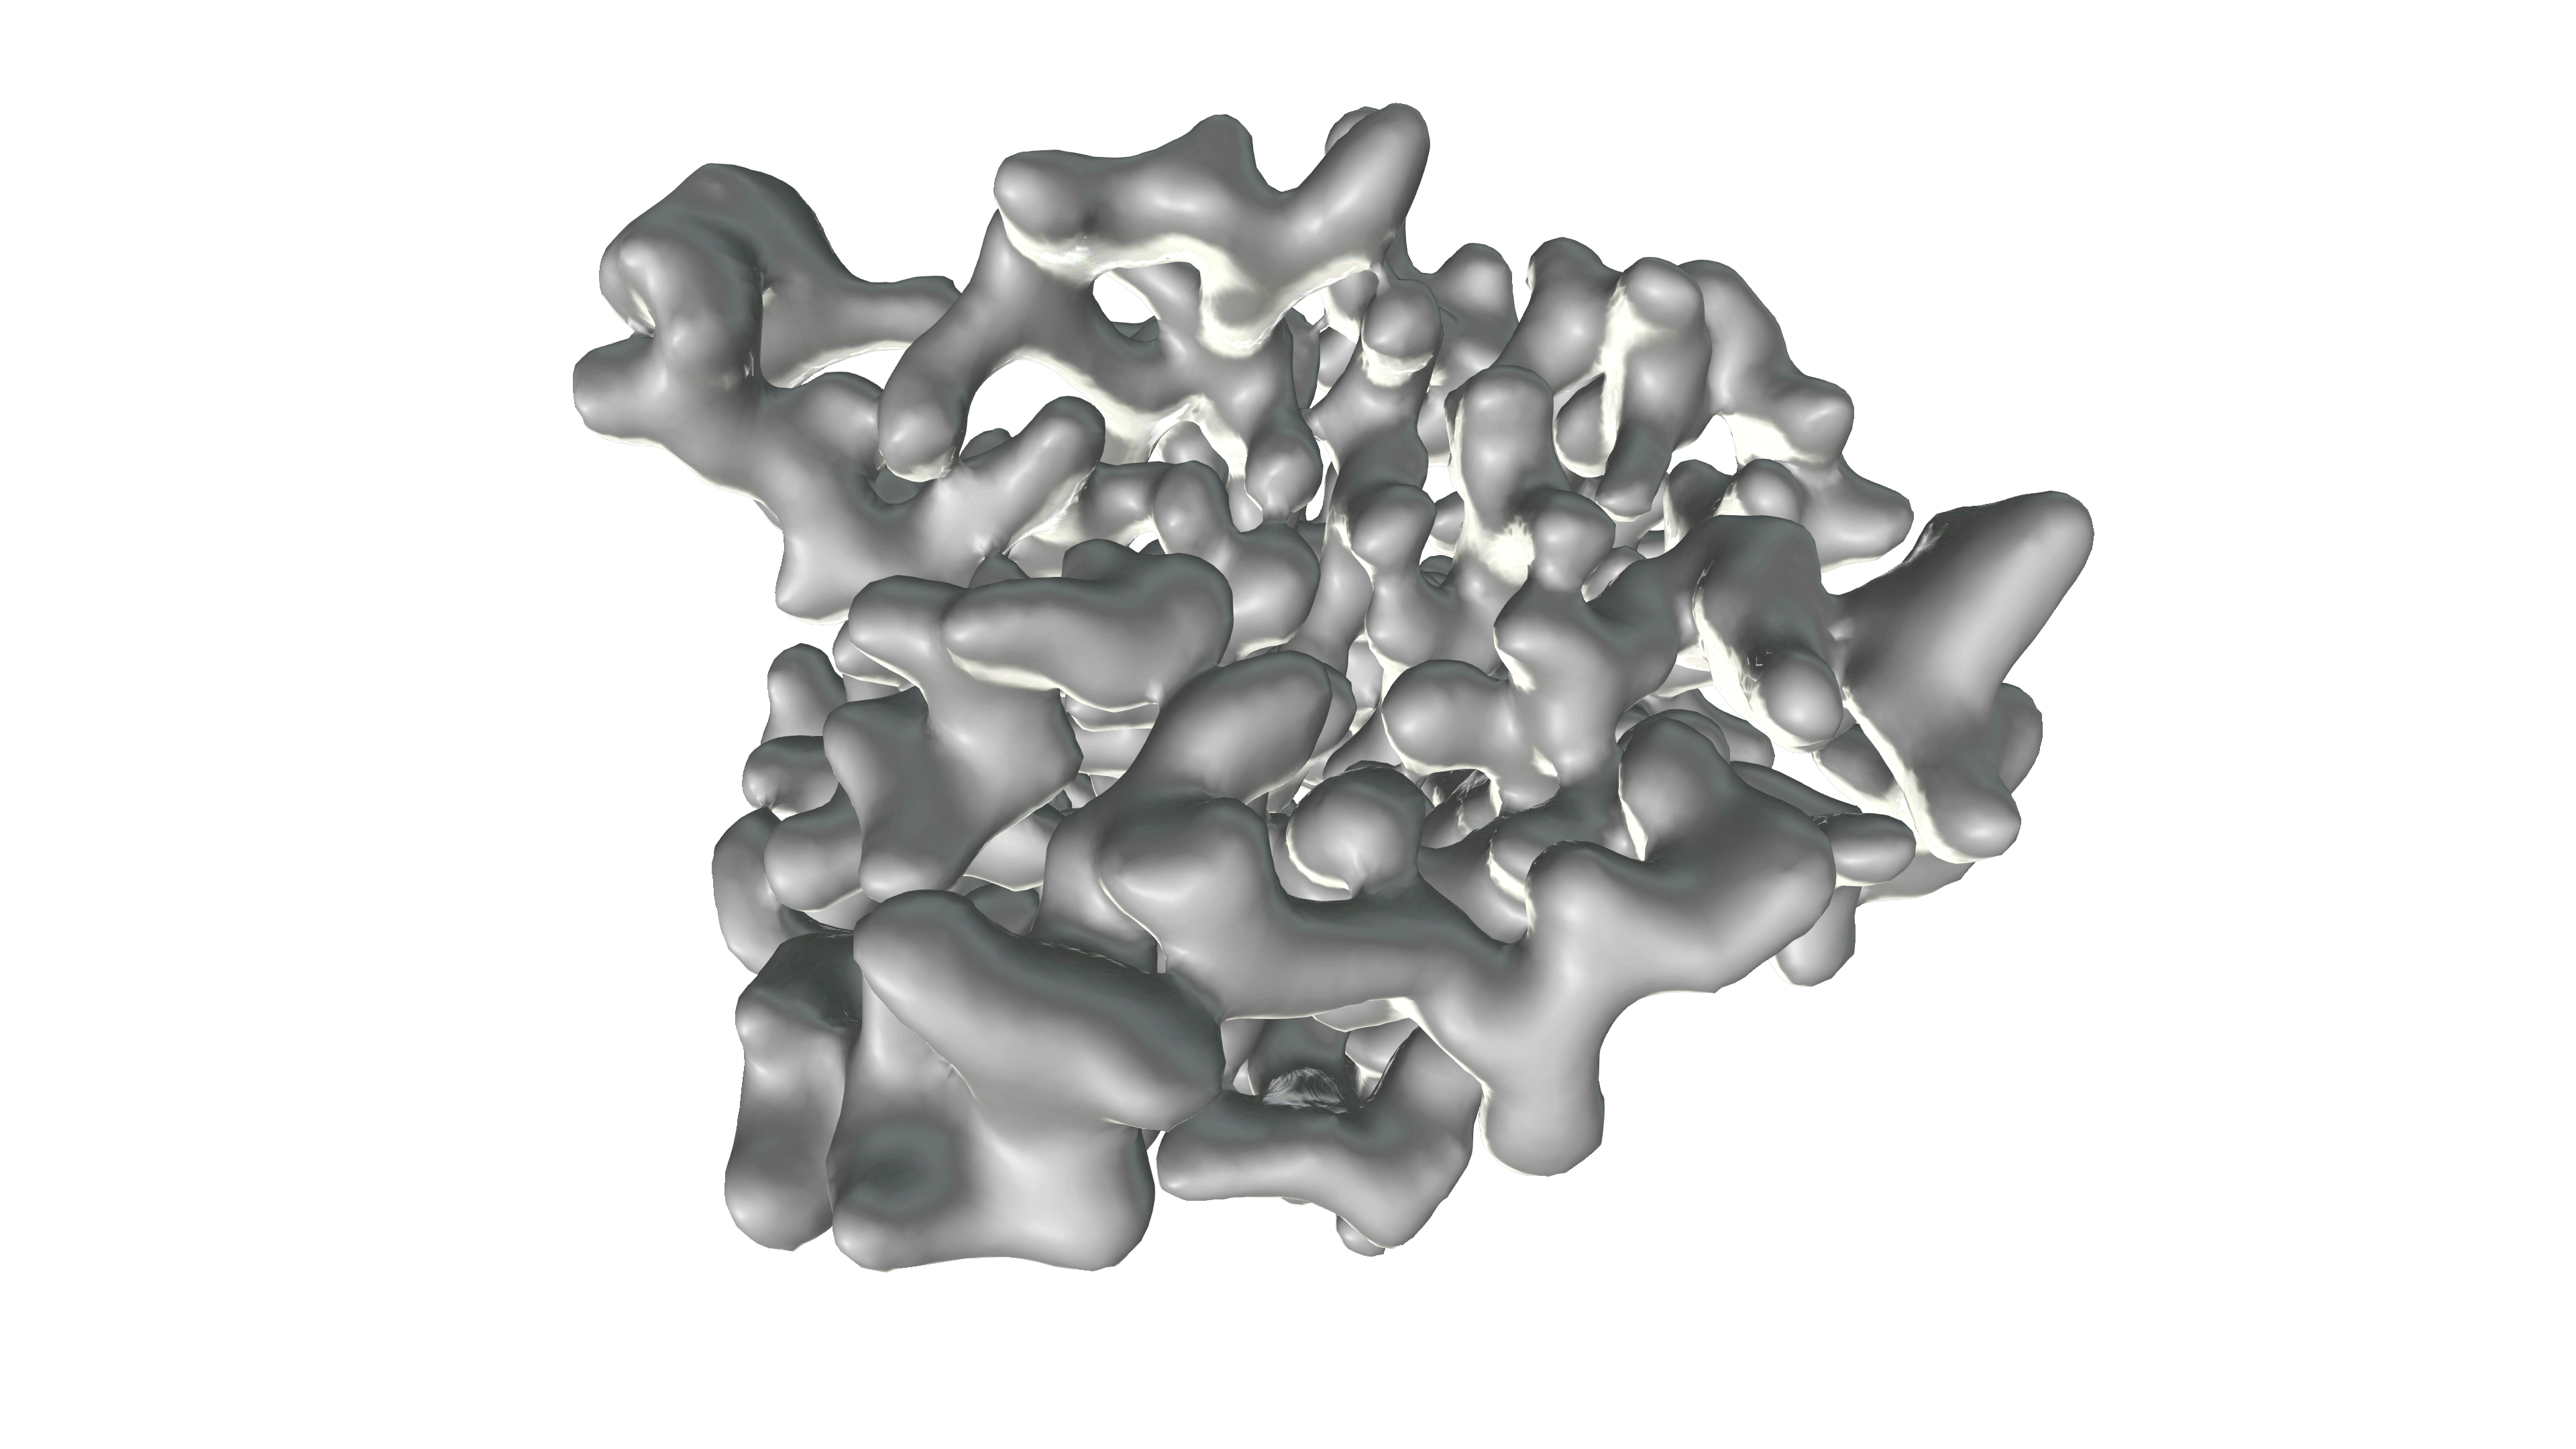
\includegraphics[width=\textwidth]{./figures/ch1/4awn_iso_1_5}
			\caption[Isosurface de densité]{\textbf{Isosurface de densité :} la surface est constituée des points de densité $1,5$.}
			\label{fig:4awn_iso_1_5}
		\end{subfigure}
		\caption[Modes de représentation moléculaire]{La désoxyribonucléase (ADNase) est une enzyme catalysant les acides désoxyribonucléiques en nucléotides ou polynucléotides. Voici quelques techniques de visualisation moléculaire, avec l'ADNase pour objet. Illustrations produites par \emph{UnityMol}~\cite{doutreligne2014unitymol} à partir d'une structure de la \emph{Protein Data Bank}~\cite{parsiegla2012structure}.}
		\label{fig:4awn_atom}
	\end{figure}
	
	
	


\cleardoublepage
\FloatBarrier
\chapter[Sélection de cibles mobiles : applications]{Sélection de cibles mobiles : quels domaines et quelles applications ?}
\minitoc
\label{appendix:annexeB}


\section{Simulations moléculaires interactives}

	\subsection{Champs de force}
	\label{sub:forceField}
	Une simulation de dynamique moléculaire s'appuie sur un \emph{champ de force}. Cette notion, propre à la chimie, est à ne pas confondre avec son homonyme en physique. Ce que l'on appelle ici un champ de forces est un ensemble de potentiels et de paramètres permettant de modéliser les interactions entre les particules simulées. Généralement, la forme fonctionnelle de base d'un champ de force s'appuie sur l'équation suivante (également illustrée par la figure~\ref{fig:ffterms}) :
	
	\begin{equation}
		\label{eq:forcefield}
		E_{totale} = E_\text{liée} + E_\text{non-liée}
	\end{equation}
	
	\begin{figure}[!htbp]
		\centering
		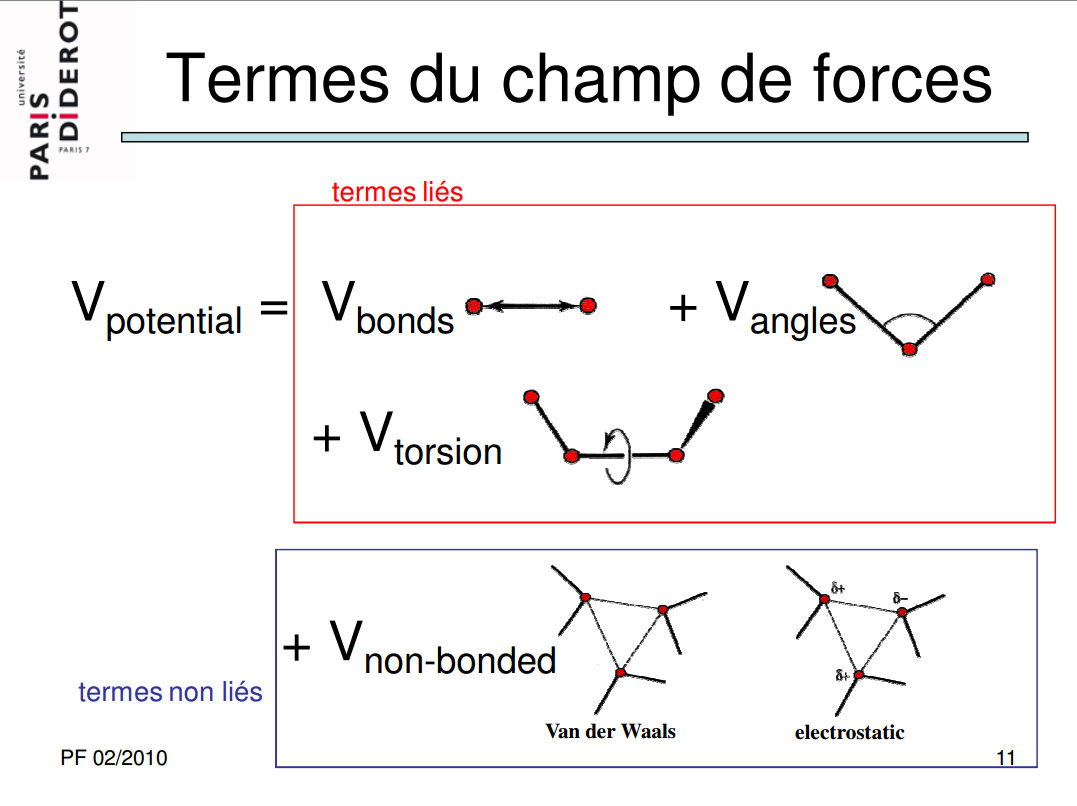
\includegraphics[width=\textwidth]{figures/ch1/ffterms}
		\caption[Termes d'un champ de forces]{Résumé des termes liés et non liés d'un champ de forces typique. Crédit : Patrick Fuchs\footnotemark.}
		\label{fig:ffterms}
	\end{figure}
	
	\footnotetext{\url{http://www.dsimb.inserm.fr/~fuchs/M1BC2T/Cours1_FF.pdf}}
	
		
	\begin{figure}[!htbp]
		%\centering
		\begin{subfigure}{.49\textwidth}
			\centering
			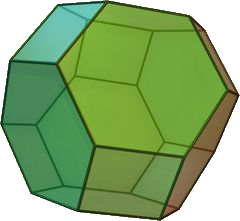
\includegraphics[height=4cm]{./figures/ch1/truncOctahedron}
			\caption{Octaèdre tronqué.}
			\label{fig:truncOctahedron}
		\end{subfigure}
		~
		\begin{subfigure}{.49\textwidth}
			\centering
			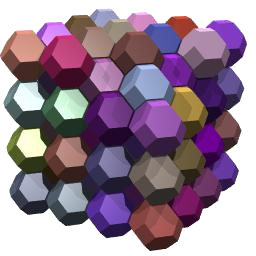
\includegraphics[height=4cm]{./figures/ch1/truncOctahedra}
			\caption{Treillis d'octaèdres tronqués.}
			\label{fig:truncOctahedra}
		\end{subfigure}
		\caption[Octaèdres pour les conditions périodiques aux limites]{Utilisation d'octaèdres pour la mise en œuvre de conditions périodiques aux limites en minimisant les erreurs et les calculs nécessaires. Crédit : S.R. Saunders, \emph{Real Wireless}\footnotemark.}
		\label{fig:octa}
	\end{figure}
	
	\footnotetext{\url{https://realwireless.wordpress.com/2008/06/03}}
	
	L'énergie totale est égale à l'énergie liée plus l'énergie non-liée, où l'énergie liée représente l'énergie des liaisons covalentes, et l'énergie non-liée représente toutes les autres interactions.
	
	\begin{equation}
		\label{eq:ebonded}
		E_\text{liée} = E_{liaison} + E_{angle} + E_\text{angle\_{}dièdre}
	\end{equation}
	
	Le terme $E_{liaison}$ correspond à l'énergie associée à la variation de la longueur d'une liaison covalente par rapport à son équilibre.%, comme l'illustre la figure~\ref{fig:e_bond}.
	
	Le terme $E_{angle}$ représente l'énergie associée à la déformation des angles formés par les paires de liaisons covalentes impliquant le même atome.% cf. la figure~\ref{fig:e_angle}.
	
	Le terme $E_\text{angle\_{}dièdre}$ correspond à l'énergie associée à la \og torsion \fg{} des liaisons covalentes centrales dans des groupes de quatre atomes.
	
	\begin{equation}
		\label{eq:nonbonded}
		E_\text{non-liée} = E_\text{électrostatique} + E_{van der Waals}
	\end{equation}
	
	Le terme $E_\text{électrostatique}$ représente l'énergie des interactions électrostatiques entre les paires d'atomes ne partageant pas de liaison covalente, telle que la décrit la loi de Coulomb~\cite{coulomb1785premier}.
	En pratique, une sommation d'Ewald, basée sur une transformation de Fourier, est souvent utilisée avec la loi de Coulomb pour le calcul des énergies électrostatiques~\cite{ewald1921berechnung, essmann1995smooth}.
	
	Le terme $E_\text{van der Waals}$ correspond à l'énergie associée aux forces de van der Waals*.
	
	Il existe de très nombreux champs de force, avec chacun ses avantages et inconvénients spécifiques, mais parmi les plus couramment utilisés, on peut citer \emph{Chemistry at HARvard Molecular Mechanics} (CHARMM)~\cite{brooks1983charmm, brooks2009charmm}, \emph{Assisted Model Building and Energy Refinement} (AMBER)~\cite{cornell1995second, wang2004development}, \emph{Optimized Potential for Liquid Simulations} (OPLS)~\cite{jorgensen1996development, kaminski2001evaluation}, ou encore \emph{GROningen MOlecular Simulation} (GROMOS)~\cite{scott1999gromos, oostenbrink2004biomolecular}.
	
	\subsection{Immersion}
	\label{sub:immersion}

	\begin{displayquote}
		Dans le langage courant, le terme d'immersion est compris comme \emph{l'exposition de l'utilisateur à un [environnement virtuel (EV)] au moyen de dispositifs occultant en partie la perception} (surtout visuelle) de l'environnement alentour, pour afficher en lieu et place une image du monde virtuel (visio-casque, salle immersive de type CAVE, etc.). Par extension, on parle d'immersion auditive, haptique, sensorielle etc. Au-delà d'un caractère informel, cette acception comporte deux ambiguïtés. D'une part, deux sémantiques différentes coexistent :
	    \begin{enumerate}
	        \item l'immersion comme \emph{l'action d'exposer l'utilisateur à un environnement simulé numériquement},
	        \item l'effet avéré ou supposé de cette exposition sur l'utilisateur.
	    \end{enumerate}
	    
	    D'autre part, en se focalisant sur l'aspect d'exposition, cet usage courant tend à centrer le problème sur la recréation d'une image artificielle proche de la situation réelle de référence, et à occulter les éventuelles interactions avec l'information persistante liée à l'environnement physique réel de l'utilisateur.	    
	\end{displayquote}

	\begin{figure}[!htbp]
		\centering
		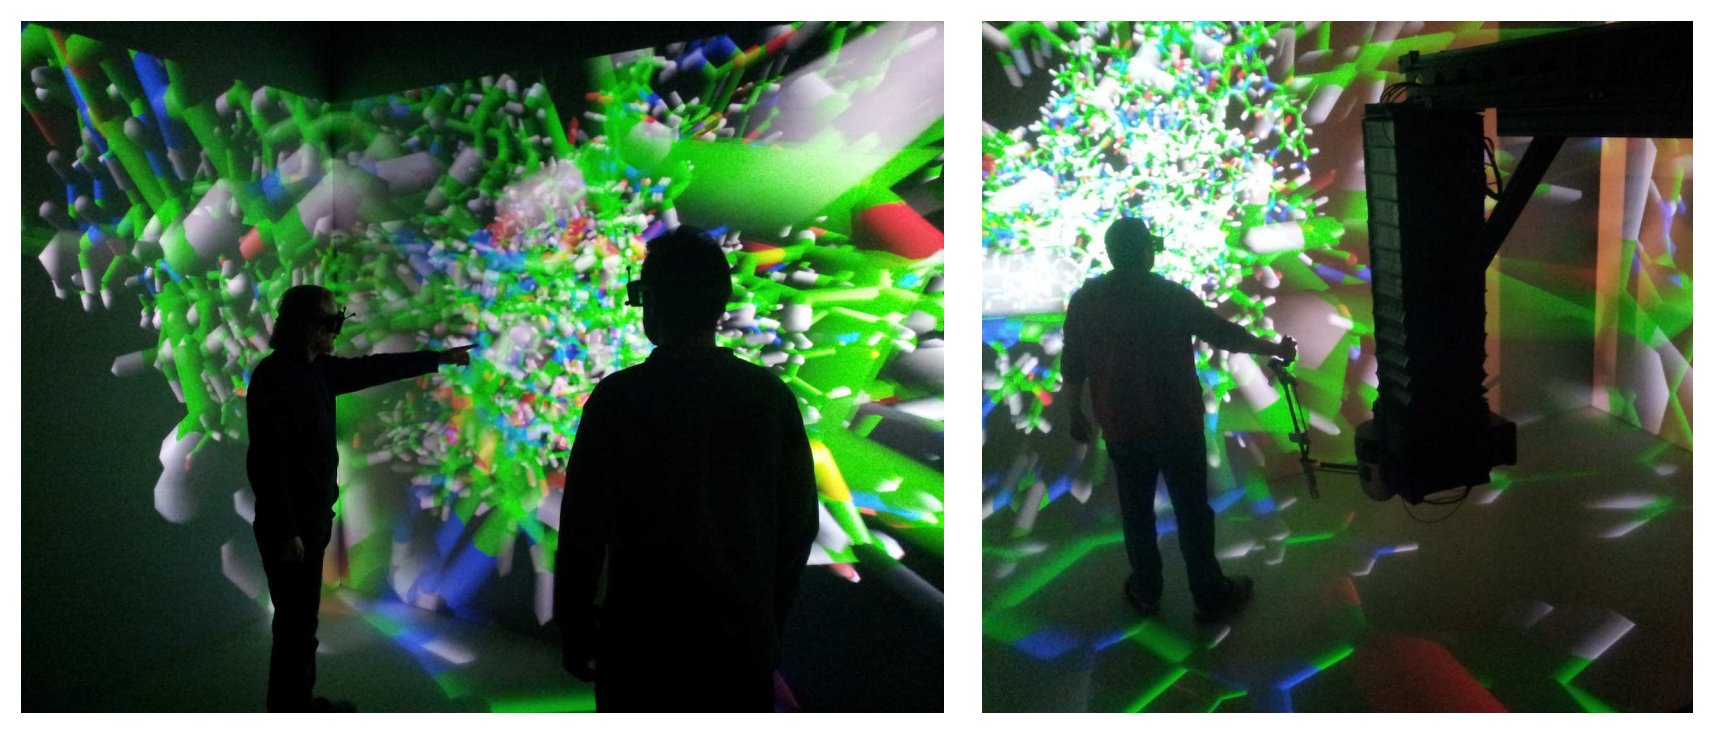
\includegraphics[width=0.9\textwidth]{figures/ch1/exaviz}
		\caption[IMD en environnement virtuel avec retour haptique, \emph{Exaviz}]{L'application \emph{Exaviz}. À gauche, deux utilisateurs dans le système EVE\footnotemark{} du groupe Venise, un CAVE multi-stéréoscopique ou deux utilisateurs peuvent avoir chacun une stéréoscopie propre à son point de vue dans la scène virtuelle. Ils peuvent ainsi collaborer et en particulier désigner avec exactitude et sans ambiguité pour l'autre utilisateur les objets virtuels. À droite, le SCALE ONE permet d'avoir des interactions avec retour d'effort dans la totalité du système EVE. Crédits :~\cite{dreher2014exaviz, cazauxsysteme}.}
		\label{fig:exaviz}
	\end{figure}
	
	\footnotetext{Un CAVE permet l'immersion dans un environnement virtuel à l'aide de vidéo-projecteurs dirigés vers trois à six des murs d'une salle parallélépipédique. Ce nom est également une référence à l'allégorie de la caverne de Platon, dans laquelle le philosophe médite et expose ses vues sur la perception, la réalité et l'illusion. Le dispositif EVE de notre équipe, Venise, ajoute le support de la multistéréoscopie et du SCALE ONE. La première est une technologie projective couplant souvent des filtrages actif (lunettes à occultation) et passif (polarisation circulaire) afin de gérer différents points de vue dans la scène virtuelle. Le second est un bras haptique à 6 degrés de liberté sur un porteur translationnel à trois degrés de liberté, produit par la société Haption.
	 
	\url{http://www.limsi.fr/venise/EVEsystem}}






\section{Contrôle de l'espace aérien}

	\begin{figure}[!htbp]
		\centering
		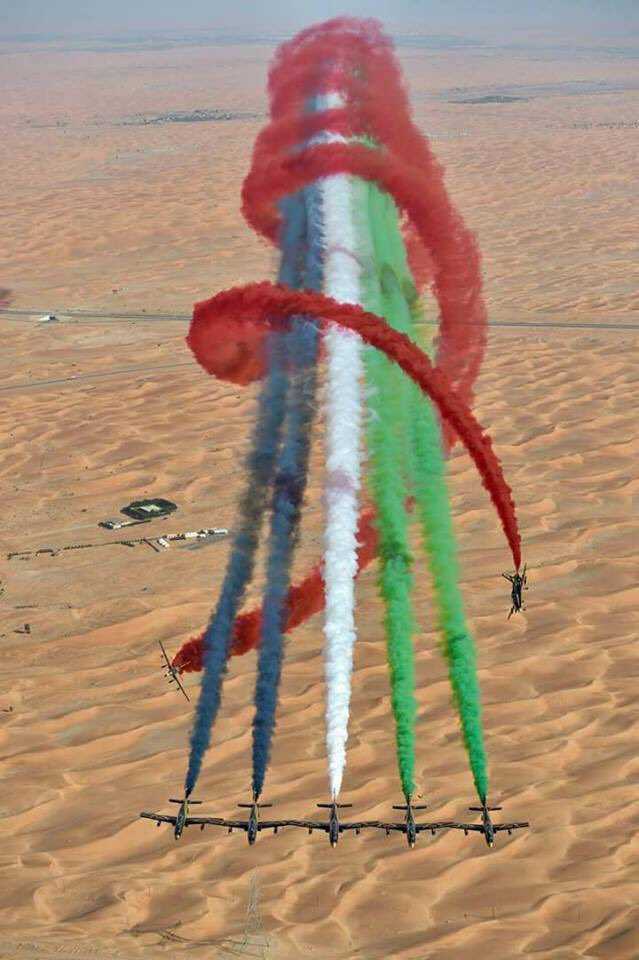
\includegraphics[width=0.8\textwidth]{figures/ch1/AlFursan}
		\caption[La patrouille acrobatique \emph{Al Fursan}]{La patrouille acrobatique émiratie \emph{Al Fursan}, avec ses trajectoires entremêlées mises en évidence par des traînées de fumée colorées. Des avions militaires peuvent avoir des trajectoires à la fois complexes, très proches les unes des autres, et parcourues à grande vitesse. Crédit : The National UAE.}
		\label{fig:alfursan}
	\end{figure}

	\newcommand{\subImgAircraftW}{0.74\textwidth}
	\begin{figure}[!htbp]
		\centering
		\begin{subfigure}[t]{\subImgAircraftW}
			\centering
			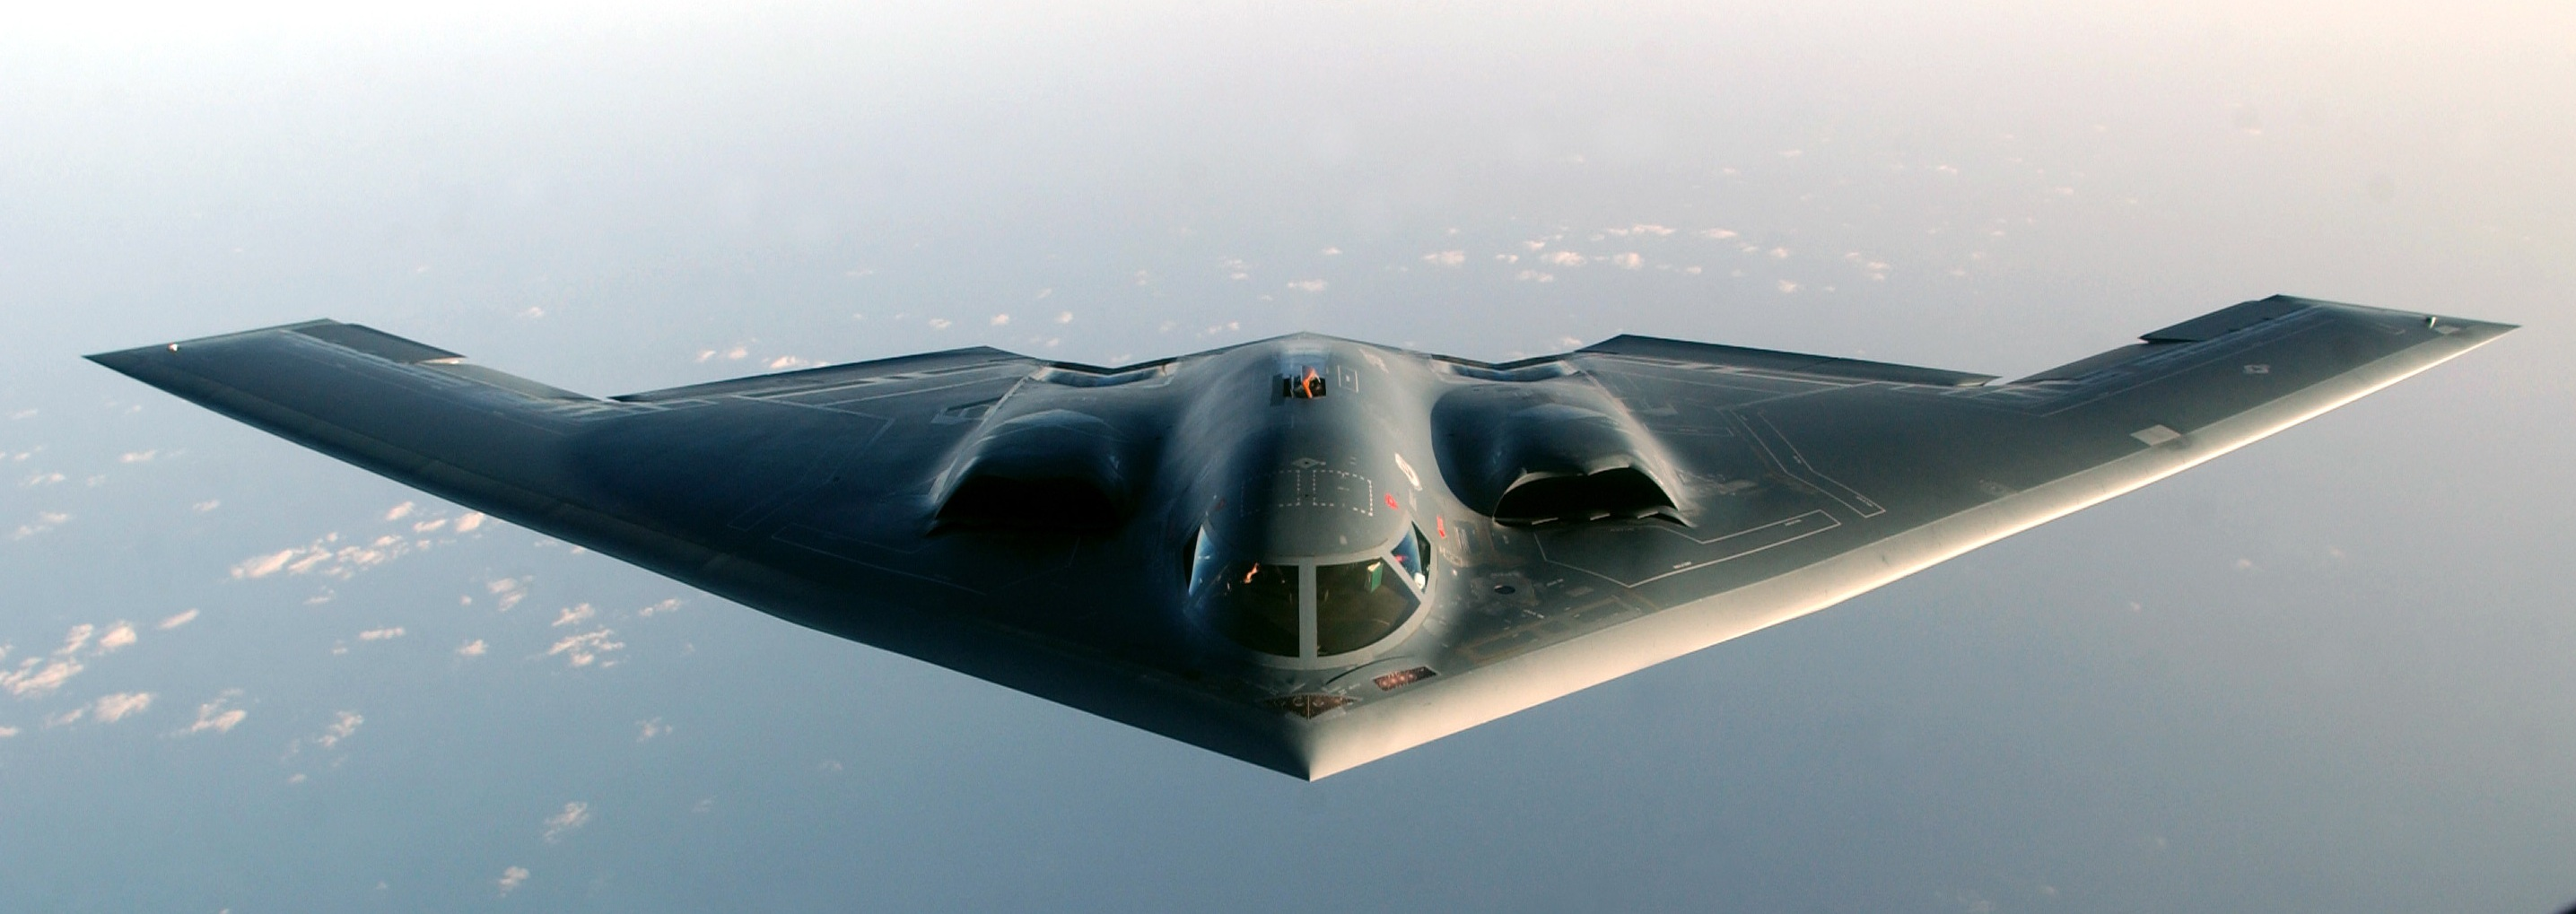
\includegraphics[width=\textwidth]{figures/ch1/B2}
			\caption[Northrop Grumman B-2 \emph{Spirit}, un bombardier stratégique furtif]{Le Northrop Grumman B-2 \emph{Spirit}, un bombardier stratégique furtif de l'USAF. Sa forme d'aile volante, son alignement de plans jamais perpendiculaires à son axe longitudinal, le placement de ses moteurs sur son dos, enfouis dans le fuselage, l'utilisation de matériaux composites absorbants, etc., contribuent à réduire la signature de cet appareil dans plusieurs bandes électromagnétiques. Crédit : \emph{Wired}.}
			\label{fig:B2}
		\end{subfigure}
		~
		\begin{subfigure}[t]{\subImgAircraftW}
			\centering
			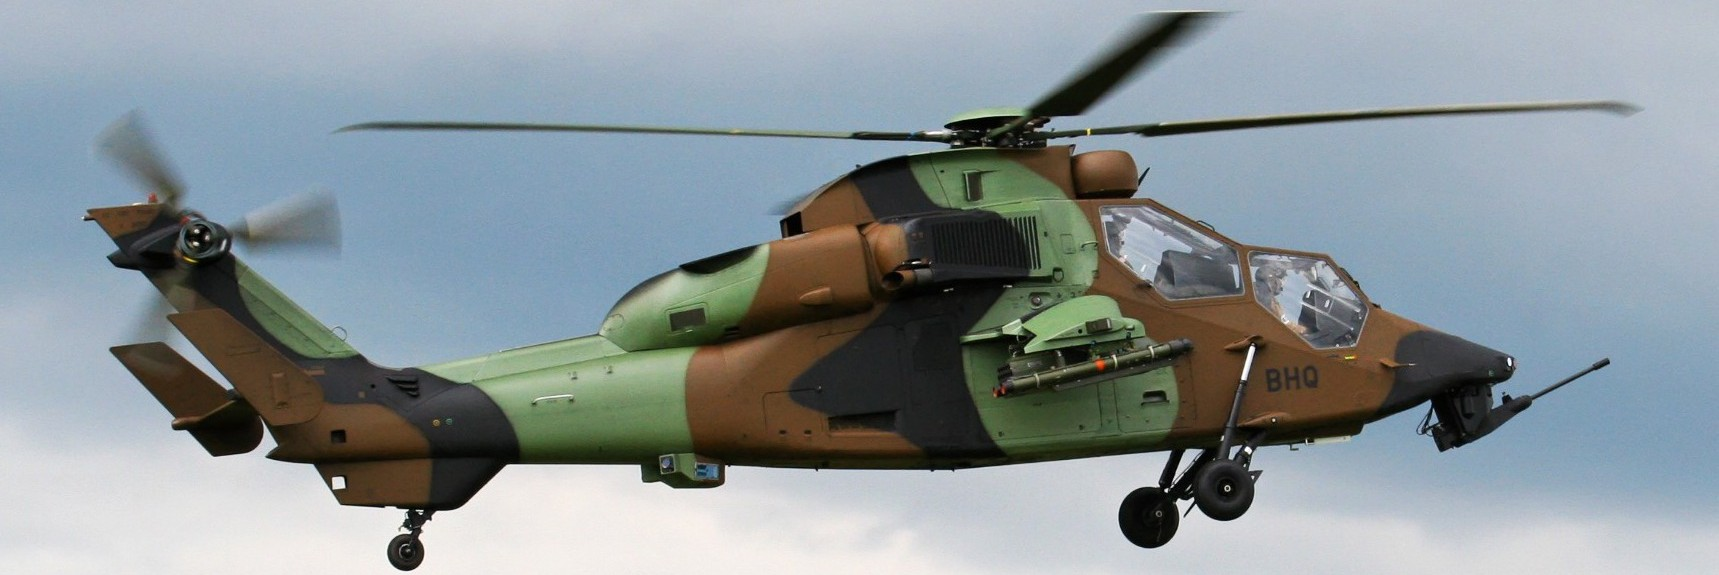
\includegraphics[width=\textwidth]{figures/ch1/tigre}
			\caption[Hélicoptère d'attaque \emph{Tigre}]{L'hélicoptère d'attaque \emph{Tigre} conçu et fabriqué par Airbus Helicopters. Cet aéronef est capable de voler jusqu'à 370~km/h en piqué, et il est assez manœuvrable pour changer de direction de vol très rapidement (sans nécessairement changer l'orientation de l'engin, par exemple en volant latéralement), voler à très basse altitude en suivant le terrain, effectuer des tonneaux, \emph{loopings}, etc., notamment grâce à sa capacité de tolérer des accélérations allant jusqu'à 4g~\cite{tigre}. Crédit : \emph{Wikimedia}}
			\label{fig:tigre}
		\end{subfigure}
		~
		\begin{subfigure}[t]{\subImgAircraftW}
			\centering
			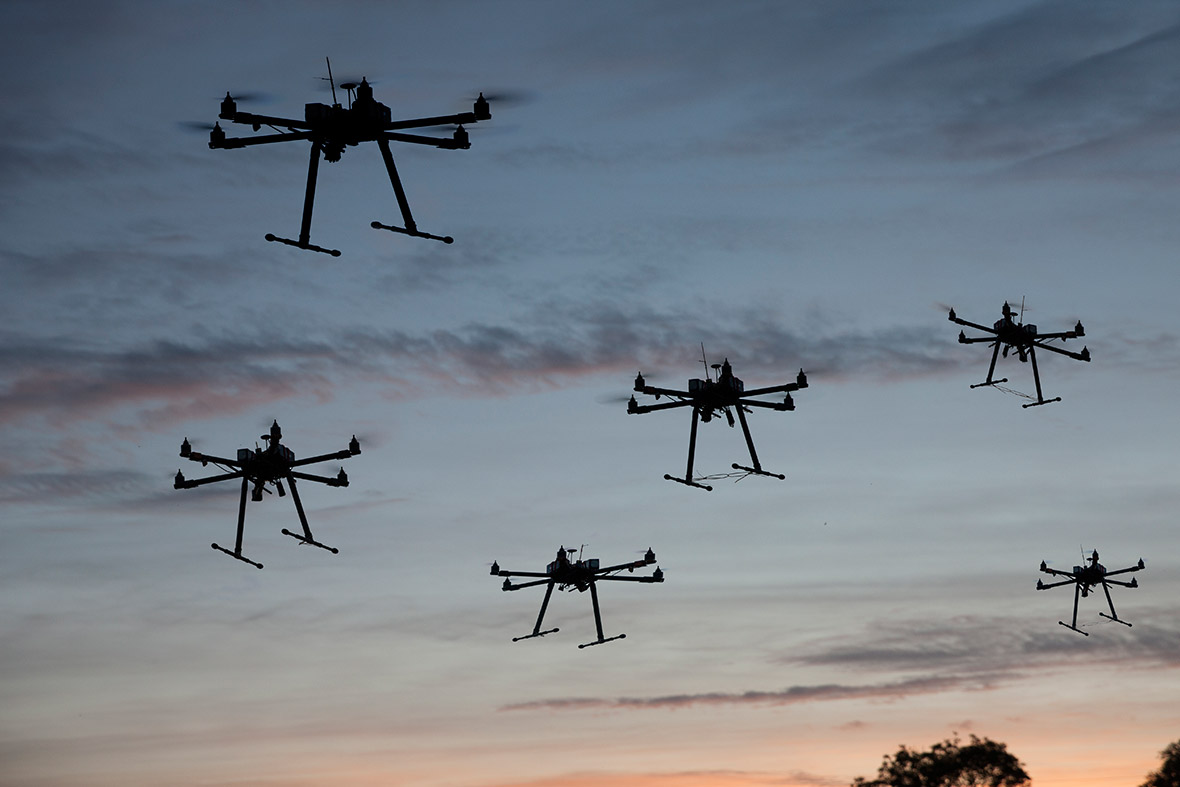
\includegraphics[width=\textwidth]{figures/ch1/swarm}
			\caption[Petit essaim de drones aériens]{Petit essaim de drones aériens. Ces engins simples et peu coûteux peuvent être produits et utilisés en très grand nombre. Ils sont souvent capables d'évoluer en formation serrée, donc de constituer un ensemble de cibles très dense. Crédit : \emph{International Business Times}.}
			\label{fig:swarm}
		\end{subfigure}
		\caption{Aéronefs militaires.}
		\label{fig:coolAircraft}
	\end{figure}

	\begin{figure}[!htbp]
		\centering
		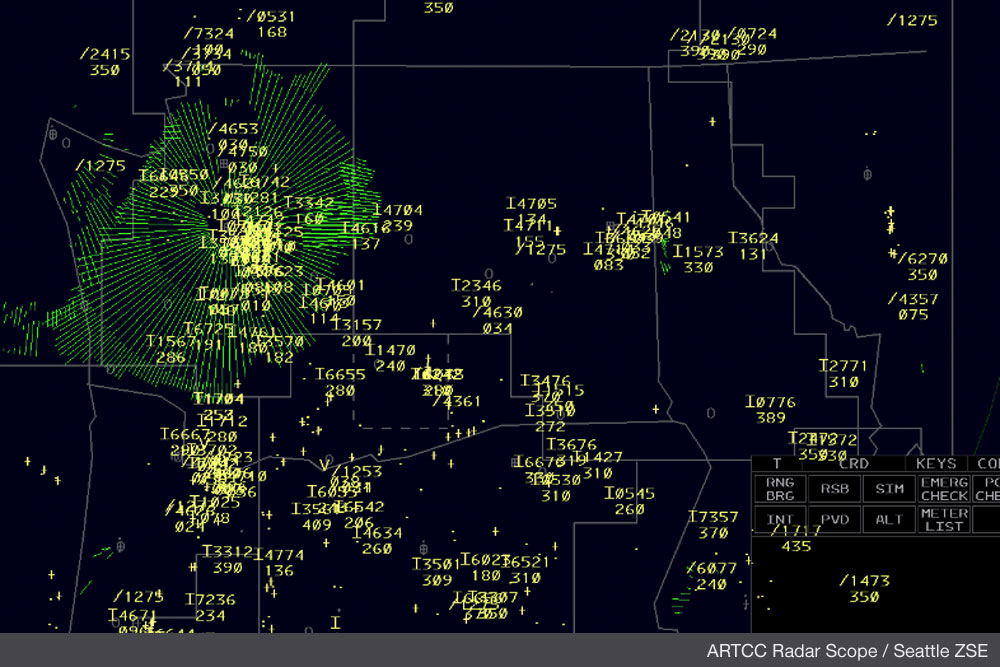
\includegraphics[width=\textwidth]{figures/ch1/Radar-Scope-ZSE}
		\caption[Écran de contrôle du trafic aérien, en 2D]{Écran de contrôle du trafic aérien. Toutes les informations, qui portent pourtant sur un espace tridimentionnel, sont représentées sur le même plan, avec une densité telle que certaines indications écrites sont illisibles. Crédit : \emph{Bold Method}.}
		\label{fig:airtraffic}
	\end{figure}
	
	\begin{figure}[!htbp]
		\centering
		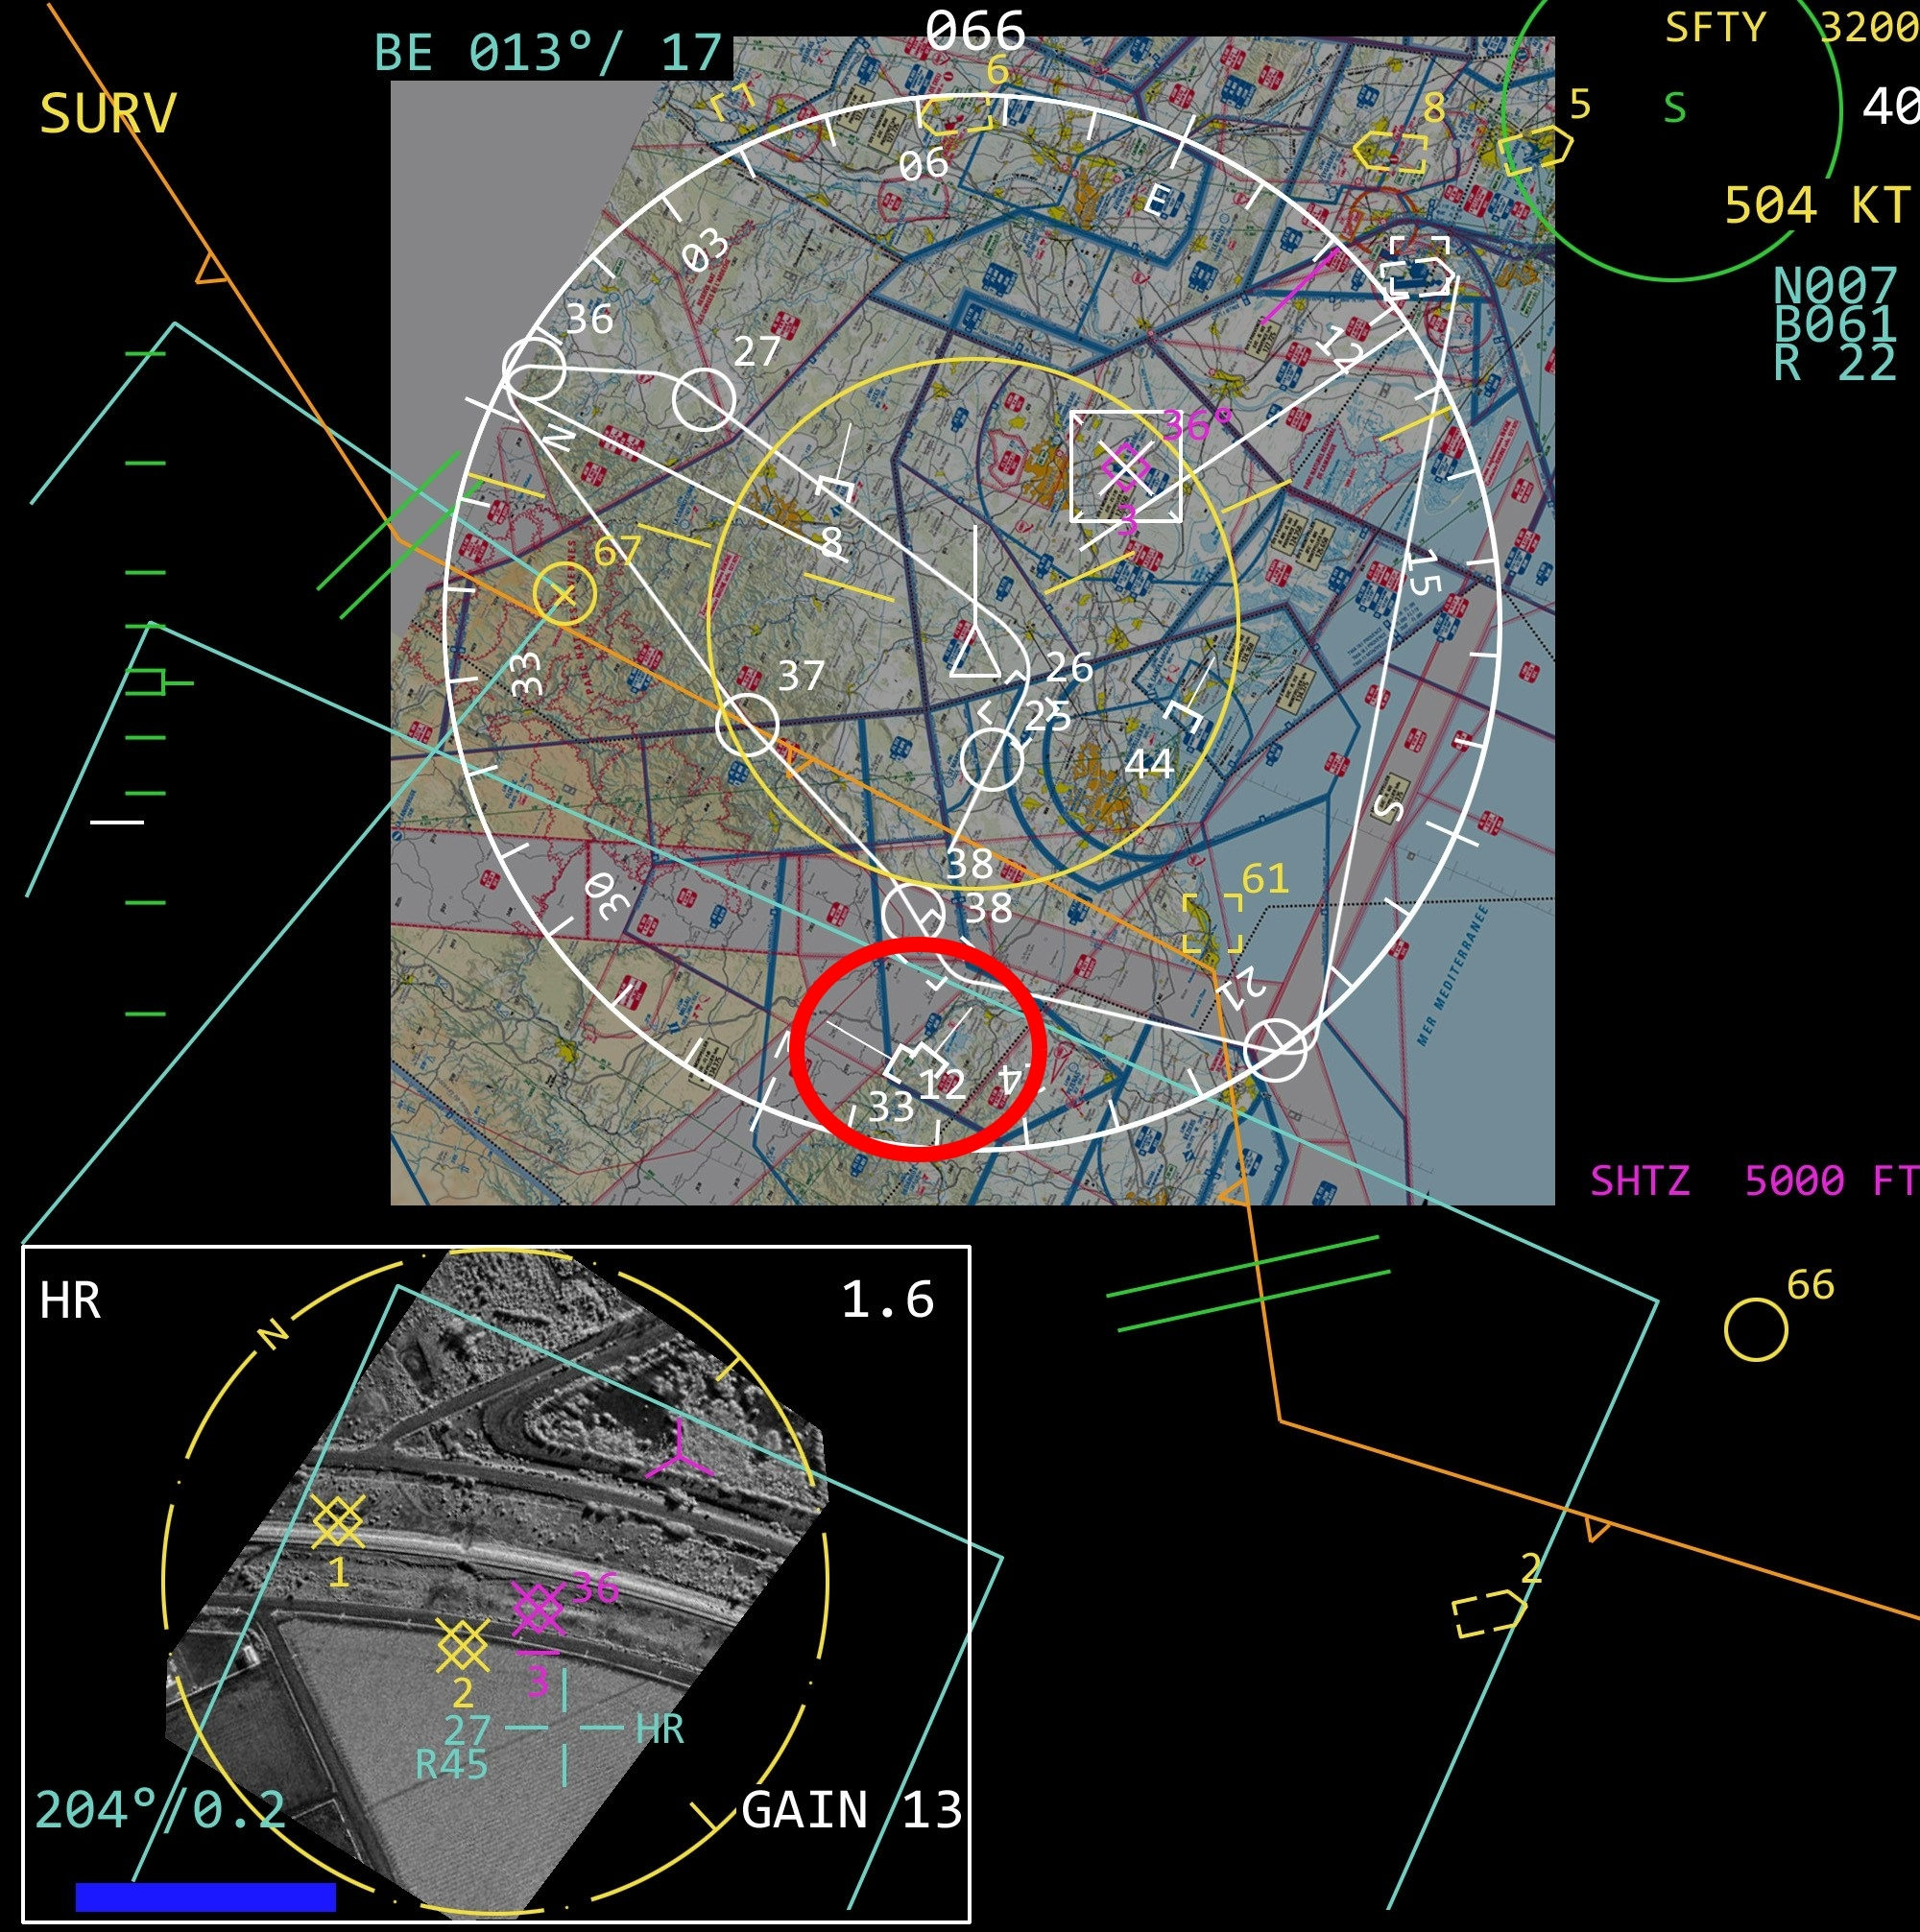
\includegraphics[width=\textwidth]{figures/ch1/sitac}
		\caption[Situation tactique vue d'un \emph{Rafale}]{Cette image représente une situation tactique telle qu'affichée sur un écran dit \og visualisation tête moyenne \fg{} dans un \emph{Rafale} de Dassault Aviation. Sur cette image très \og chargée \fg{} seuls deux petits symboles, que nous avons ici entourés en rouge, représentent des avions ennemis. Au-delà de la carte de fond, les autres symboles représentent diverses informations tactiques importantes : l'avion lui-même bien sûr, sa direction, un compas de route, l'altitude maximale des obstacles terrestres, l'échelle, la vitesse de l'avion, le plan de vol, la ligne de front, un zoom, etc. Par conséquent, même avec un très petit nombre de cibles potentielles, l'affichage est complexe, dense, et potentiellement gênant pour la sélection. Crédit : Portail Aviation\footnotemark.}
		\label{fig:sitac}
	\end{figure}
	
	\footnotetext{\url{http://www.portail-aviation.com/2015/07/exclusif-a-la-decouverte-de-la-situation-tactique-du-rafale-sitac.html}}
	
	\subsection{F-15E et Mi-24}
	\label{sub:f15e}
	Pendant la guerre du Golfe, par exemple, un F-15E \emph{Strike Eagle} se trouva dans l'impossibilité de verrouiller son radar sur un hélicoptère Mi-24 \emph{Hind} irakien pour l'abattre à l'aide d'un missile, du fait de la proximité du Mi-24 au sol et de la vivacité de ses mouvements. L'officier des systèmes d'armes du F-15E dut basculer vers la nacelle de désignation laser pour \og marquer \fg{} l'hélicoptère afin de le détruire à l'aide d'une bombe~\cite{craig2007debrief}. Il ne précise pas si cette désignation fut difficile, du fait de l'utilisation d'un outil conçu pour cibler des objets statiques ou, à la rigueur, lents.
	
	\footnotetext{\url{https://theaviationist.com/2016/02/14/f-15e-shot-down-iraqi-mi-24}}
	
	Observons tout de même que le F-15E est un appareil biplace dans lequel l'officier des systèmes d'armes a pour tâche principale de détruire les cibles ennemies, pendant que le pilote man\oe{}uvre l'appareil. Dans un avion monoplace, ces deux tâches doivent être remplies par une seule personne. Il est donc d'autant plus important que chaque tâche soit aussi facile que possible. Ajoutons enfin qu'avec ses 12 tonnes, le Mil Mi-24 est un hélicoptère lourd et nettement moins man\oe{}uvrable que des appareils plus récents comme un \emph{Tigre} de 6 tonnes, par exemple.
	
\FloatBarrier

\section{Contrôle de l'espace extra-atmosphérique}

	\begin{figure}[!htbp]
		%\centering
        \begin{subfigure}[t]{0.41\textwidth}
            \centering
            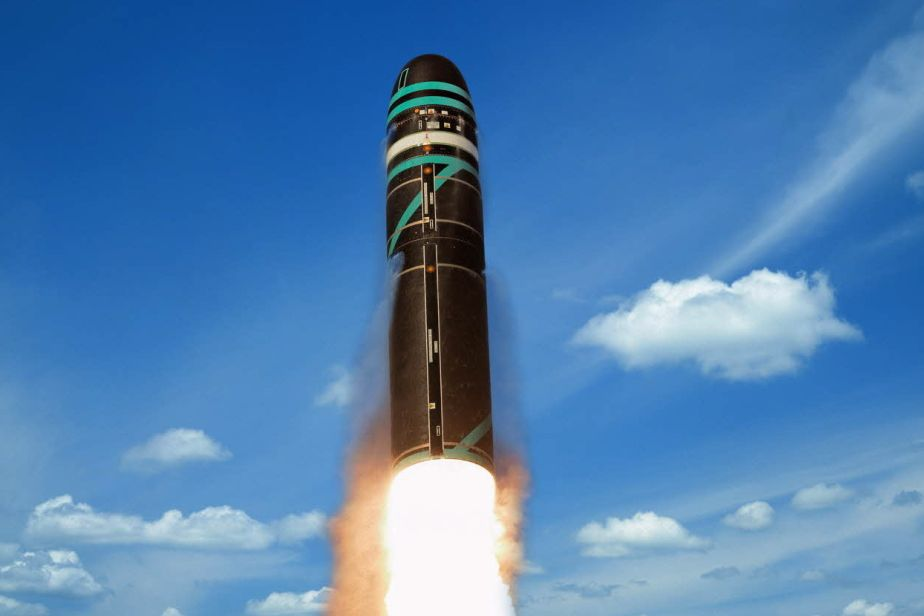
\includegraphics[width=\textwidth]{figures/ch1/m51}
        	\caption[Missile français M51]{Tir du missile balistique français M51, depuis un sous-marin. Son altitude de croisière est d'environ 1000~km et sa vitesse maximale serait de Mach~25\footnotemark. Crédit : \emph{Defence Talk}\footnotemark.}
            \label{fig:m51}
        \end{subfigure}
        ~
        \begin{subfigure}[t]{0.57\textwidth}
            \centering
            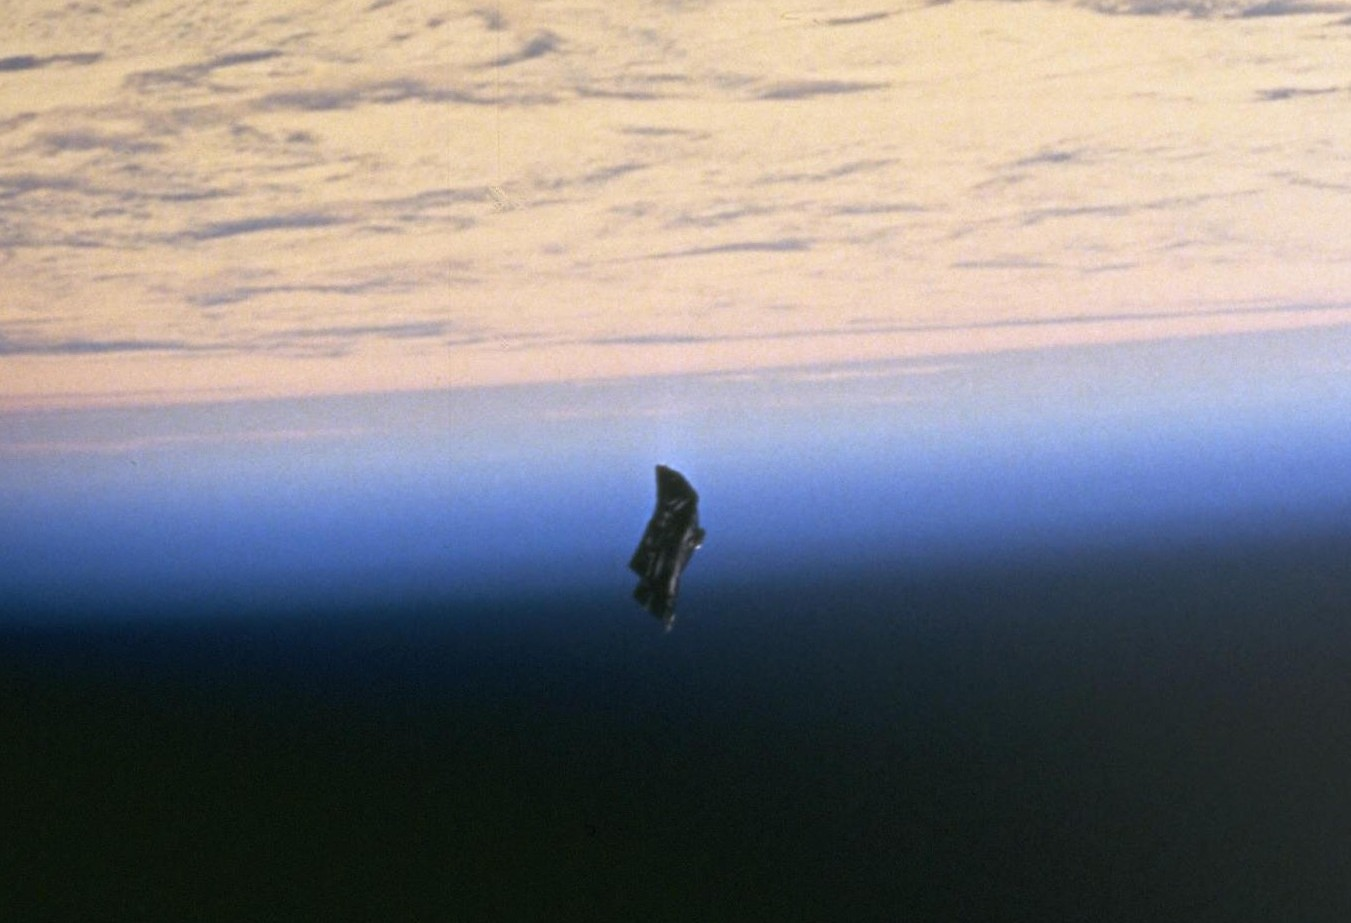
\includegraphics[width=\textwidth]{figures/ch1/space_debris_zoom}
            \caption[Débris spatial]{Débris spatial : une couverture thermique à la dérive en orbite terrestre. Crédit : NASA\protect\footnotemark.}
            \label{fig:spaceDeb}
        \end{subfigure}
        \label{fig:aerospace}
        \caption{Objets aérospatiaux.}
	\end{figure}
	
	\addtocounter{footnote}{-2}
	\footnotetext{\url{http://www.techno-science.net/?onglet=glossaire&definition=12366}}
	\addtocounter{footnote}{1}
	\footnotetext{\url{http://www.defencetalk.com/french-m51-ballistic-missile-self-destructs-in-failed-test-47689}}
	\addtocounter{footnote}{1}
	\footnotetext{\url{https://eol.jsc.nasa.gov/SearchPhotos/photo.pl?mission=STS088&roll=724&frame=66}}



\section{Vidéo-surveillance}

	\begin{figure}[!htbp]
		%\centering
		\begin{subfigure}[t]{0.49\textwidth}
			\centering
			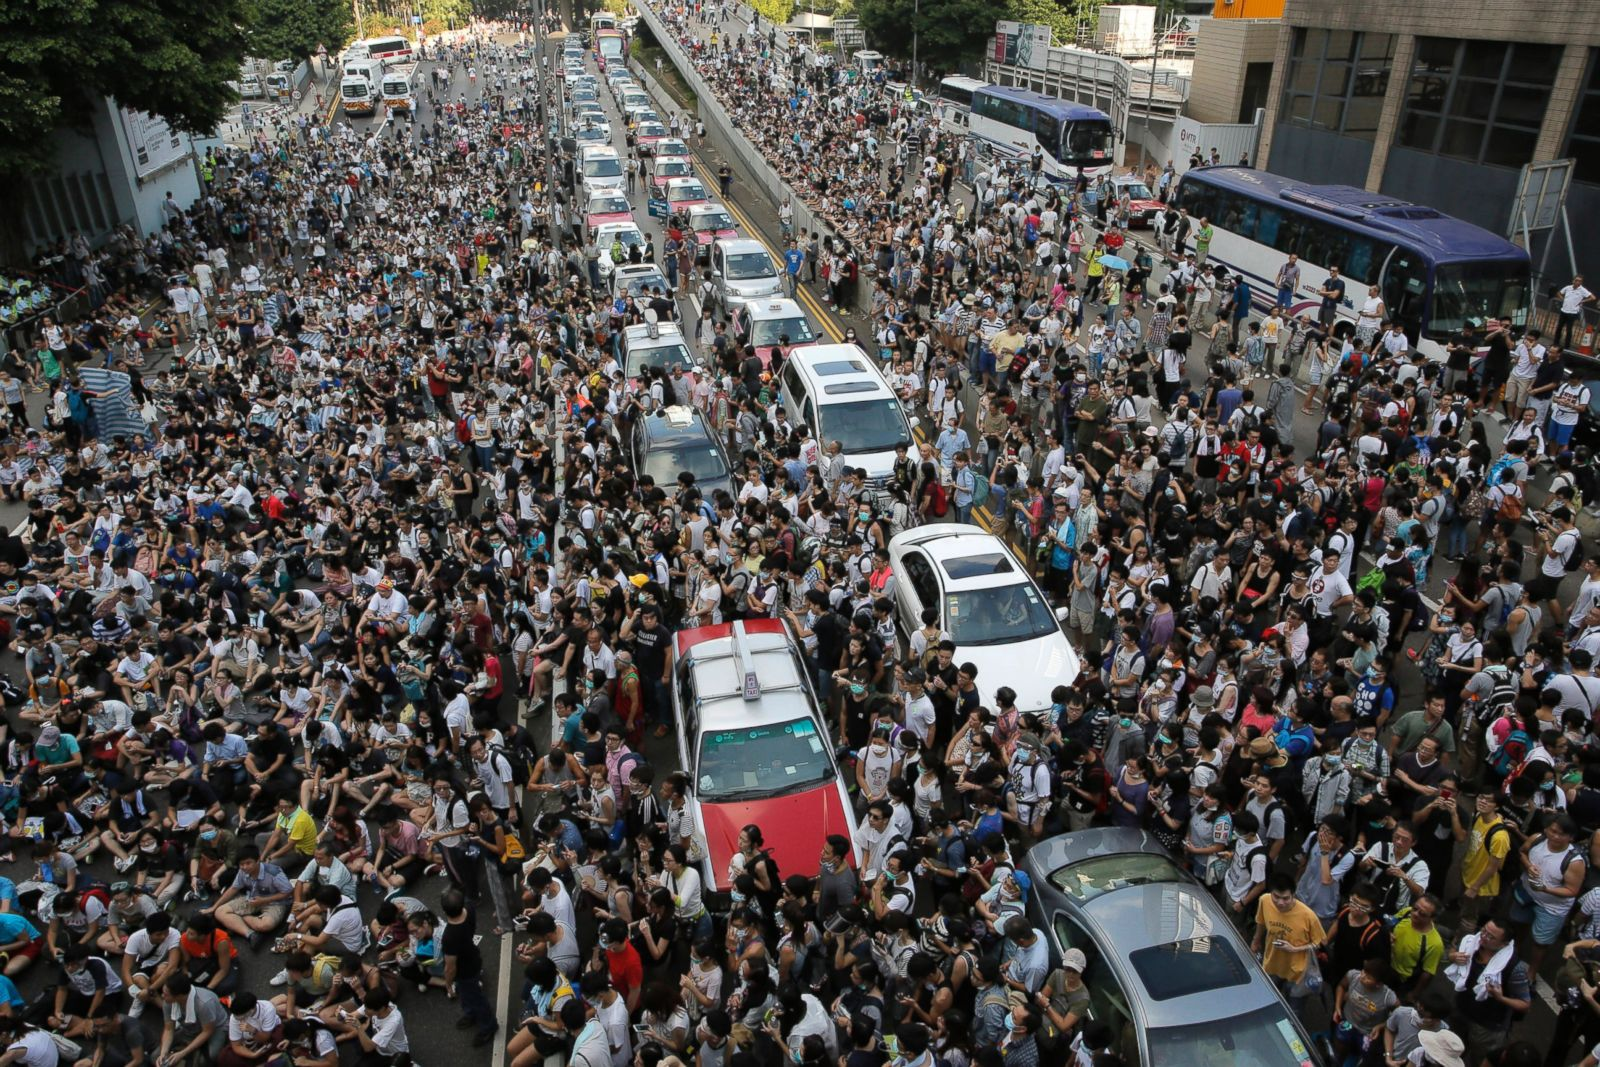
\includegraphics[width=\textwidth]{figures/ch1/crowdhk}
			\caption[Foule de manifestants à Hong-Kong]{Foule de manifestants à Hong-Kong. Ils sont presque immobiles, mais d'une densité très élevée. Crédit : \emph{ABC News}.}
			\label{fig:crowdhk}
		\end{subfigure}
		~
		\begin{subfigure}[t]{0.49\textwidth}
			\centering
			\includegraphics[width=\textwidth]{figures/ch1/crowdacdc}
			\caption[Foule à un concert]{Foule à un concert du groupe AC/DC. Le mouvement presque nul, mais la densité de cibles est extrêmement élevée. Crédit : \emph{SHP Online}\footnotemark.}
			\label{fig:crowdacdc}
		\end{subfigure}
		\label{fig:crowds}
		\caption{Foules.}
	\end{figure}
	

	\footnotetext{\url{http://www.shponline.co.uk/understanding-crowds-and-crowded-space-issues}}






	


\section{Surveillance électromagnétique}
	\label{sub:deveryware}

	\begin{displayquote}
		Deveryware est depuis 2003 la spécialiste de référence pour le développement et le déploiement de solutions mettant en œuvre la géolocalisation en temps réel des personnes et des biens.

		Elle est un partenaire important de l'État français pour des applications régaliennes utilisant ces techniques, qu'il s'agisse de sécurité publique ou de sécurité civile pour contribuer à la mise en sécurité des citoyens.\footnotemark{}
	\end{displayquote}
	
	\footnotetext{\url{http://www.deveryware.com/savoir-faire/notre-expertise}}

	\begin{figure}[!htbp]
		\centering
		\includegraphics[width=\textwidth]{figures/ch1/cellphones}
		\caption[Surveillance des signaux de téléphones portables]{Système de surveillance en temps réel des signaux de téléphones portables, tiré de la série télévisée \emph{Le Bureau des légendes}\footnotemark{}, et inspiré de systèmes réels. Sur cette vue d'Alger, chaque point coloré représente la position d'un téléphone dont le signal est localisé. Le nombre de cibles potentielles est très élevé, et la densité peut être extrême par endroits.}
		\label{fig:cellphones}
	\end{figure}
	
	\footnotetext{\OE{}uvre réalisée par Éric Rochant et produite par Canal+.}


	


\section{Jeux vidéo}

	\subsection{Jeux de tir}
	\begin{figure}[!htbp]
		%\centering
		\begin{subfigure}[t]{0.49\textwidth}
			\centering
			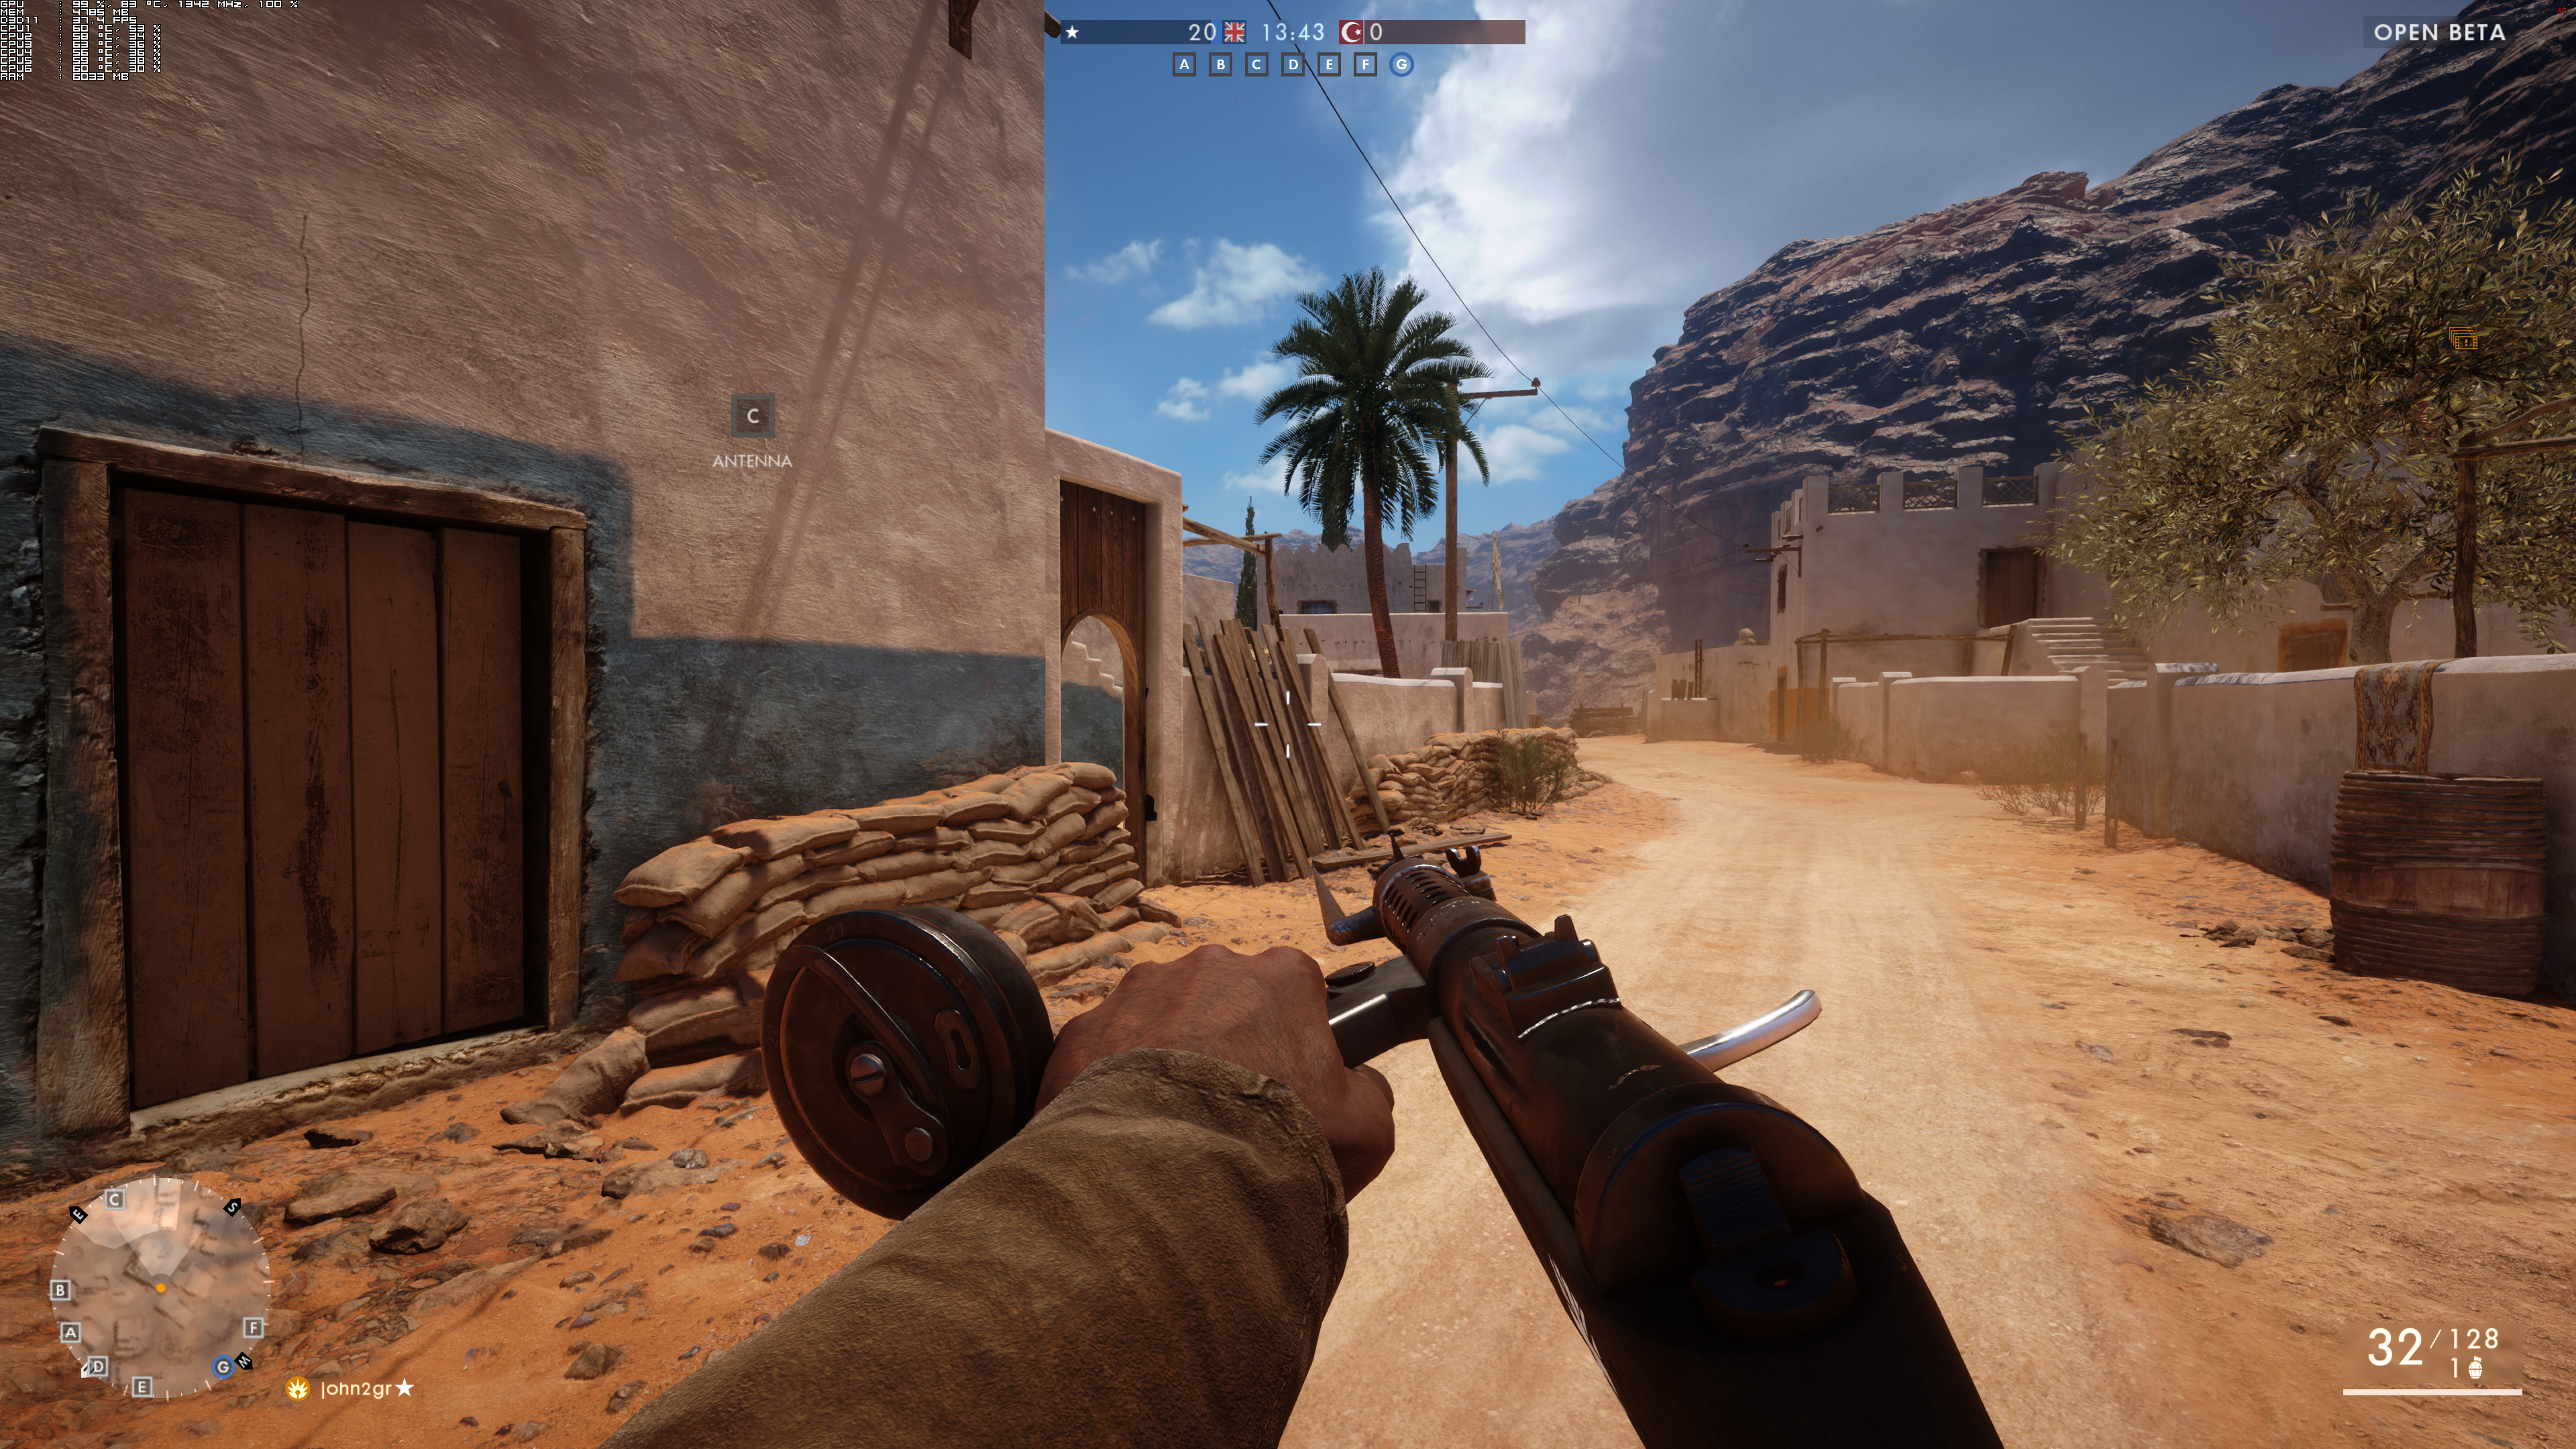
\includegraphics[width=\textwidth]{figures/ch1/bf1}
			\caption{\emph{Battlefield 1}. Des ennemis peuvent surgir n'importe quand, de n'importe où, et le joueur devra réagir avec vitesse et précision. Développé par EA DICE et édité par Electronic Arts.}
			\label{fig:bf1}
		\end{subfigure}
		~
		\begin{subfigure}[t]{0.49\textwidth}
			\centering
			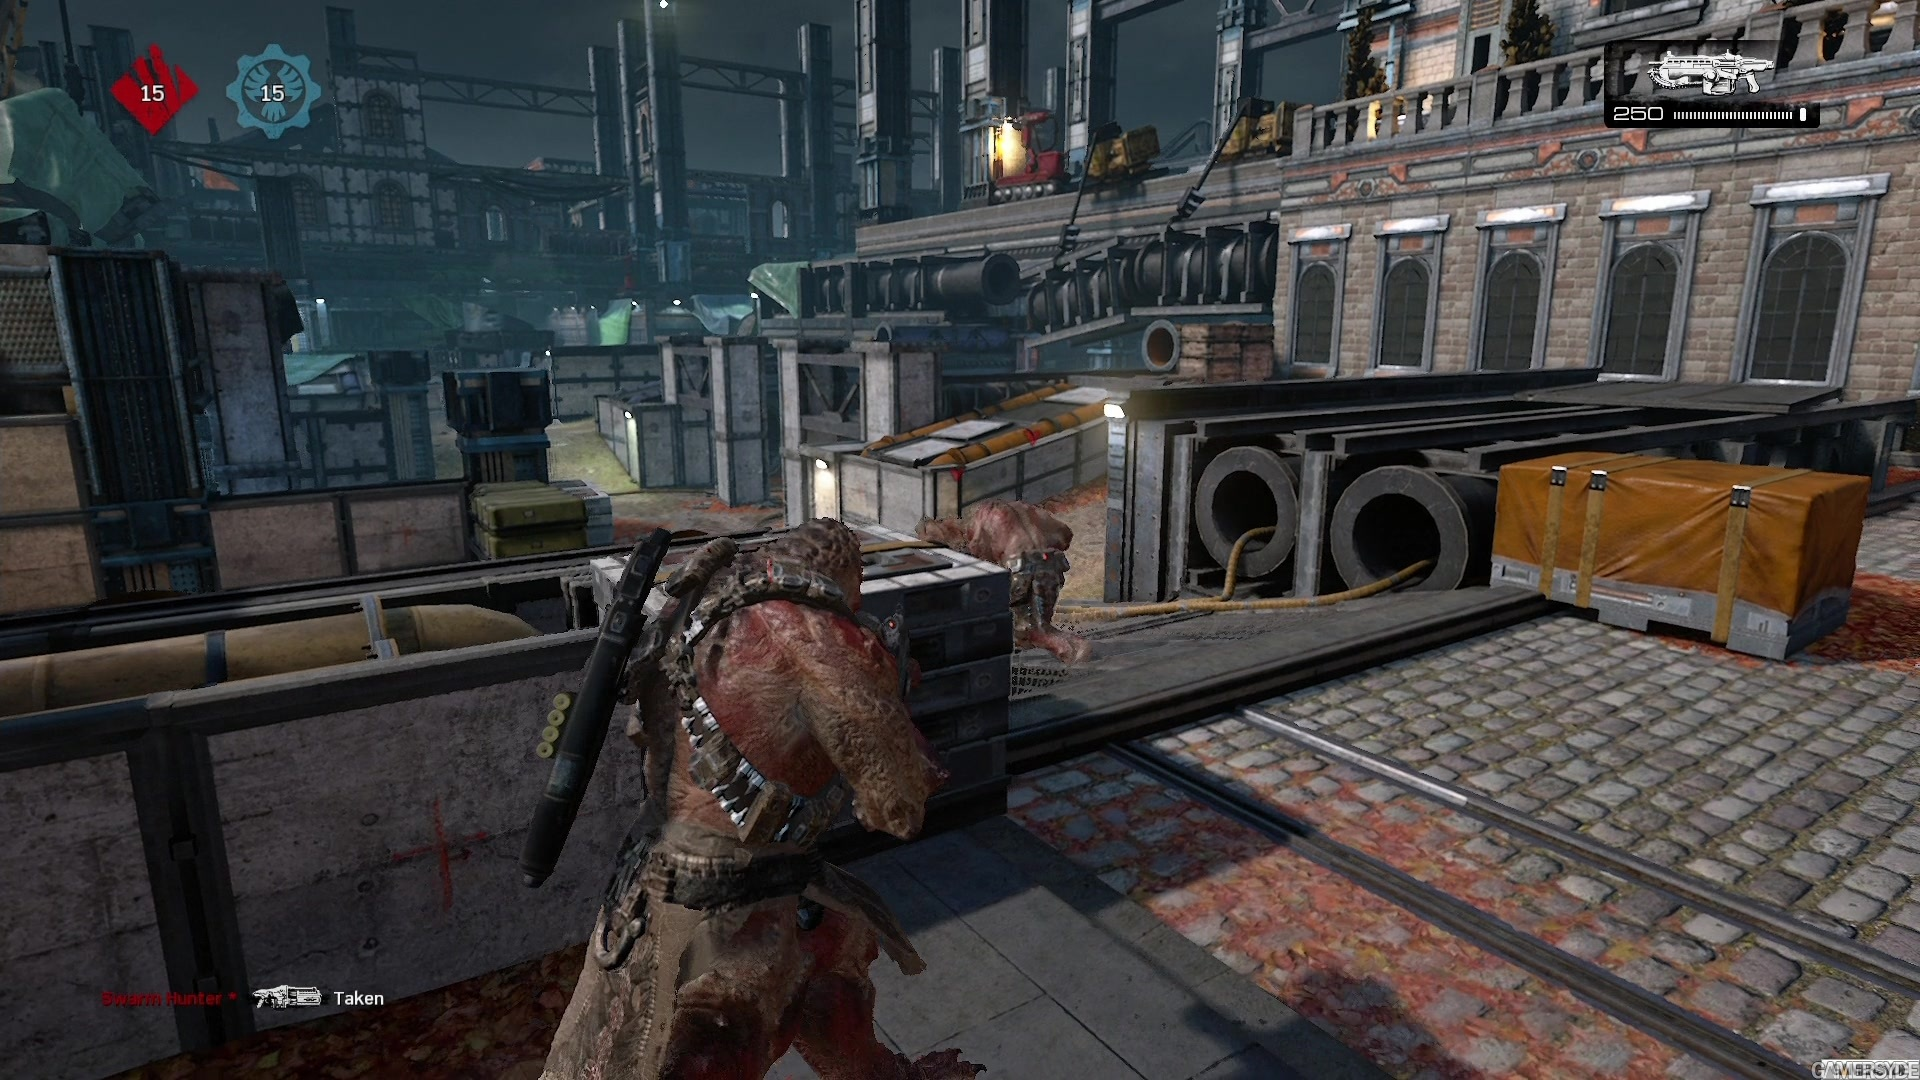
\includegraphics[width=\textwidth]{figures/ch1/gears}
			\caption{\emph{Gears of War 4}. La caméra est placée derrière le personnage, au-dessus et sur le côté. Jeu développé par The Coalition et édité par Microsoft Studios.}
			\label{fig:gears}
		\end{subfigure}
		\caption{Jeux de tir.}
		\label{fig:shooters}
	\end{figure}
	
	
	
	
	\subsection{Jeux de rôle d'action (ARPG)}
	
	\begin{figure}[!htbp]
		%\centering
		\begin{subfigure}[t]{0.48\textwidth}
			\centering
			
\includegraphics[width=\textwidth]{figures/ch1/f4vats}
			\caption[Système V.A.T.S permettant de faciliter les tirs dans \emph{Fallout 4}]{Dans l'ARPG \emph{Fallout 4}, le système V.A.T.S. permet ici au joueur de cibler tranquillement la tête de cette créature, pendant que le temps est ralenti. Le tir aura une probabilité de succès de 77~\%{}, dérivée des compétences de tir du personnage contrôlé, et des circonstances du combat à cet instant précis. Jeu édité par Bethesda Softworks, et développé par ses propres studios.}
			\label{fig:f4vats}
		\end{subfigure}
		~
		\begin{subfigure}[t]{0.50\textwidth}
			\centering
			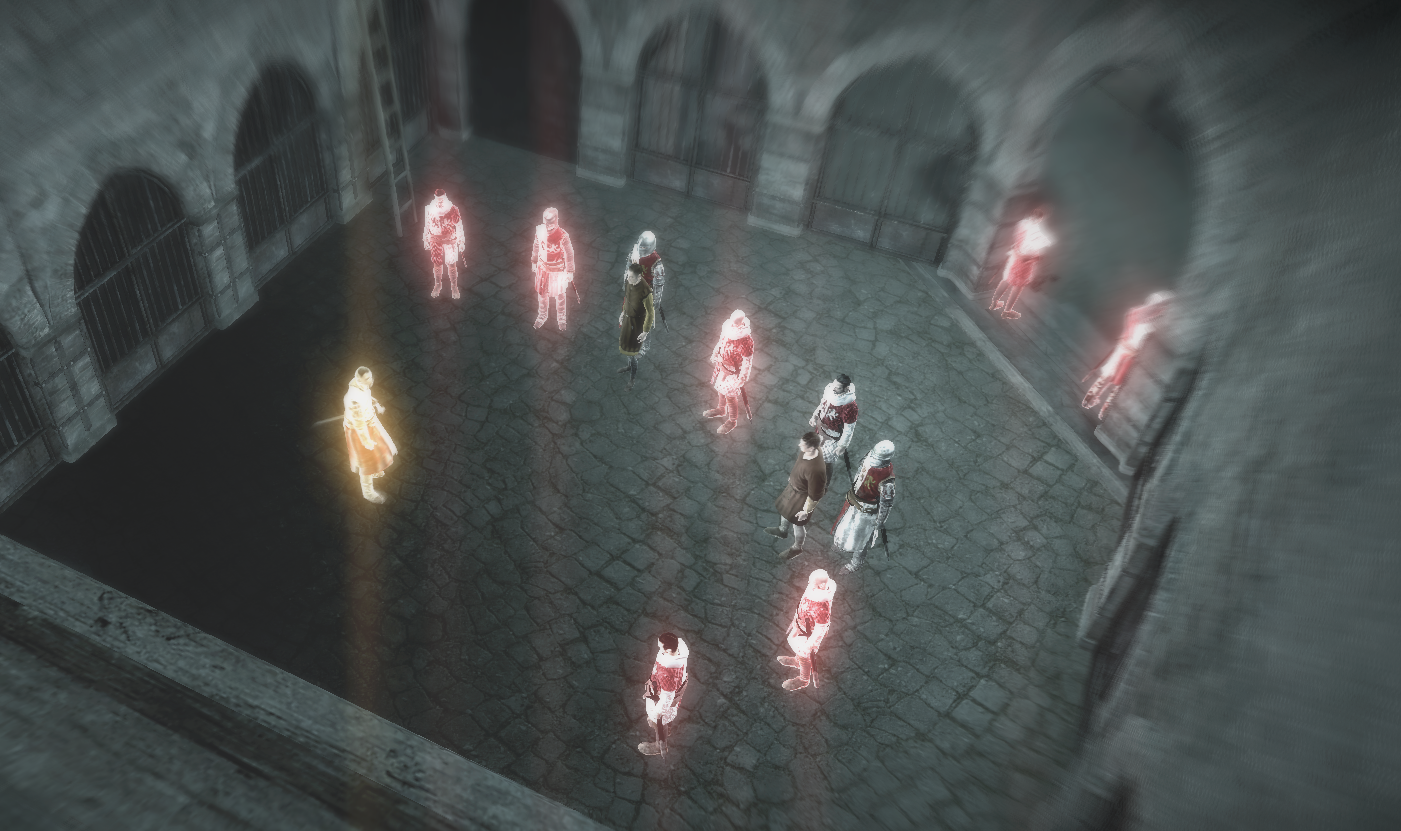
\includegraphics[width=\textwidth]{figures/ch1/assassin}
			\caption[Système \emph{Eagle Vision} dans le jeu \emph{Assassin's Creed}] {\emph{Assassin's Creed} : le joueur peut voir les personnages à travers les obstacles, connaître leur nature grâce à leur couleur, et désigner la cible que le personnage attaquera ensuite semi-automatiquement. Si les cibles elles-mêmes ne sont ni très rapides ni très imprévisibles, à leurs mouvements absolus s'ajoutent ceux du joueur, qui ne dispose généralement que d'un petit \emph{joystick} sous son pouce pour viser. Édité et développé par Ubisoft.}
			\label{fig:ac_ev}
		\end{subfigure}
		\label{fig:gamesTargeting}
		\caption{Techniques d'assistance à la visée ou sélection dans les jeux vidéo.}
	\end{figure}
	
	
	
	
	\subsubsection{Jeux de gestion, de stratégie (RTS) et de tactique (RTT)}

	\begin{figure}[!htbp]
		\begin{subfigure}[t]{\textwidth}
			\centering
			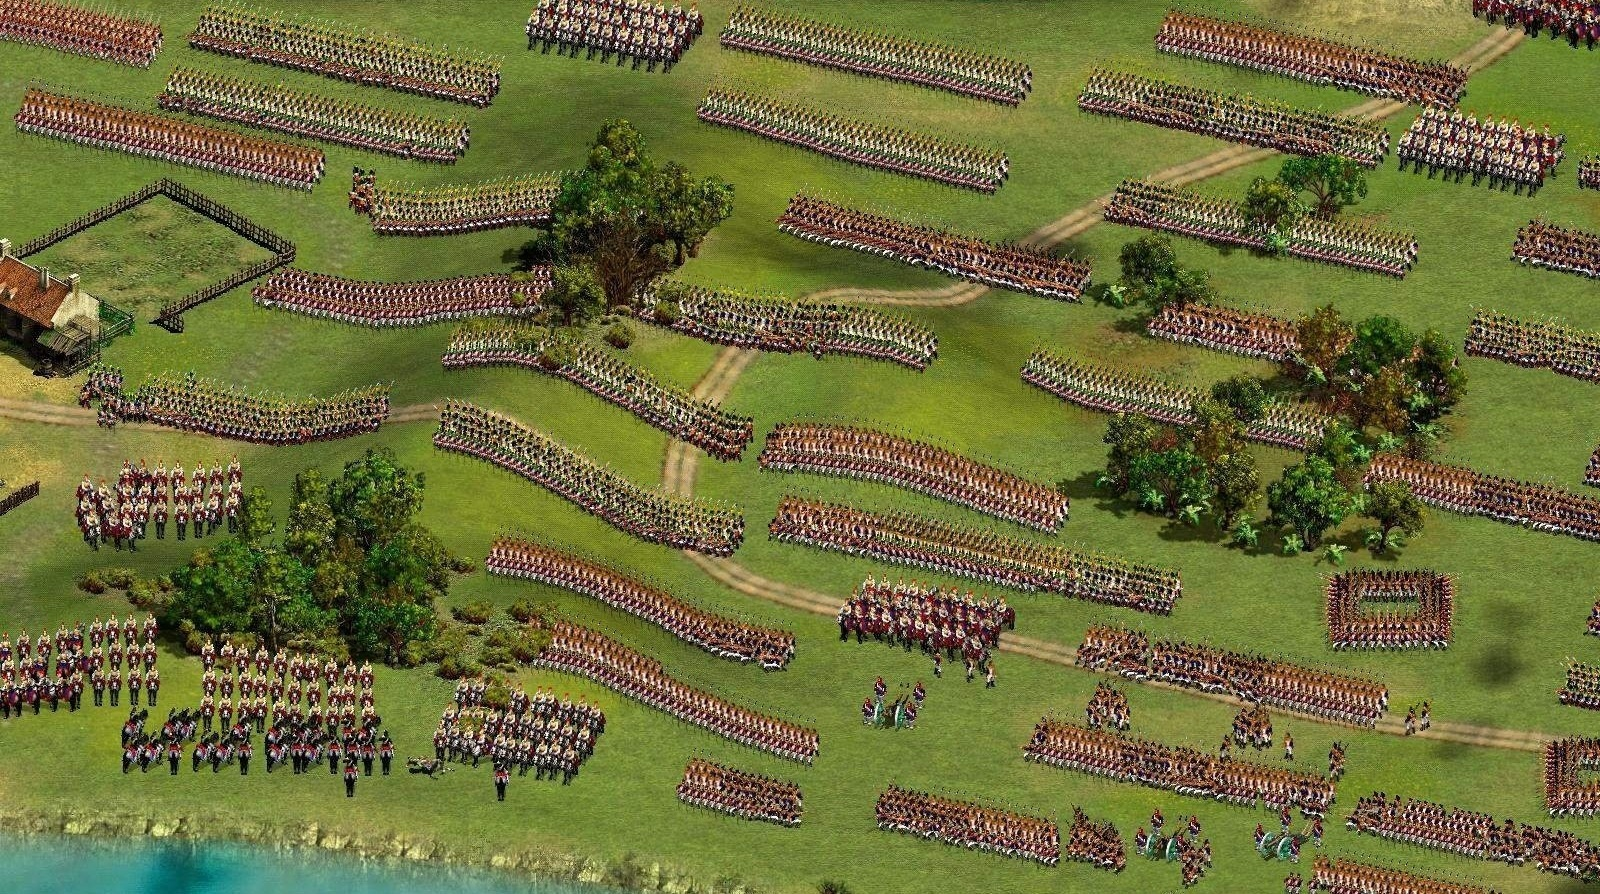
\includegraphics[width=\textwidth]{figures/ch1/cossacks2}
			\caption[Un RTS avec de très nombreuses unités : \emph{Cossacks~II: Napoleonic Wars}]{\emph{Cossacks~II: Napoleonic Wars} : les unités sont nombreuses, très proches les unes des autres. Au nombre et à la densité s'ajouteront, pendant la bataille, le mouvement, le désordre et le mélange avec des unités ennemies. Développé par GSC Game World et édité par CDV Software.}
			\label{fig:cossacks2}
		\end{subfigure}
		~
		\begin{subfigure}[t]{\textwidth}
			\centering
			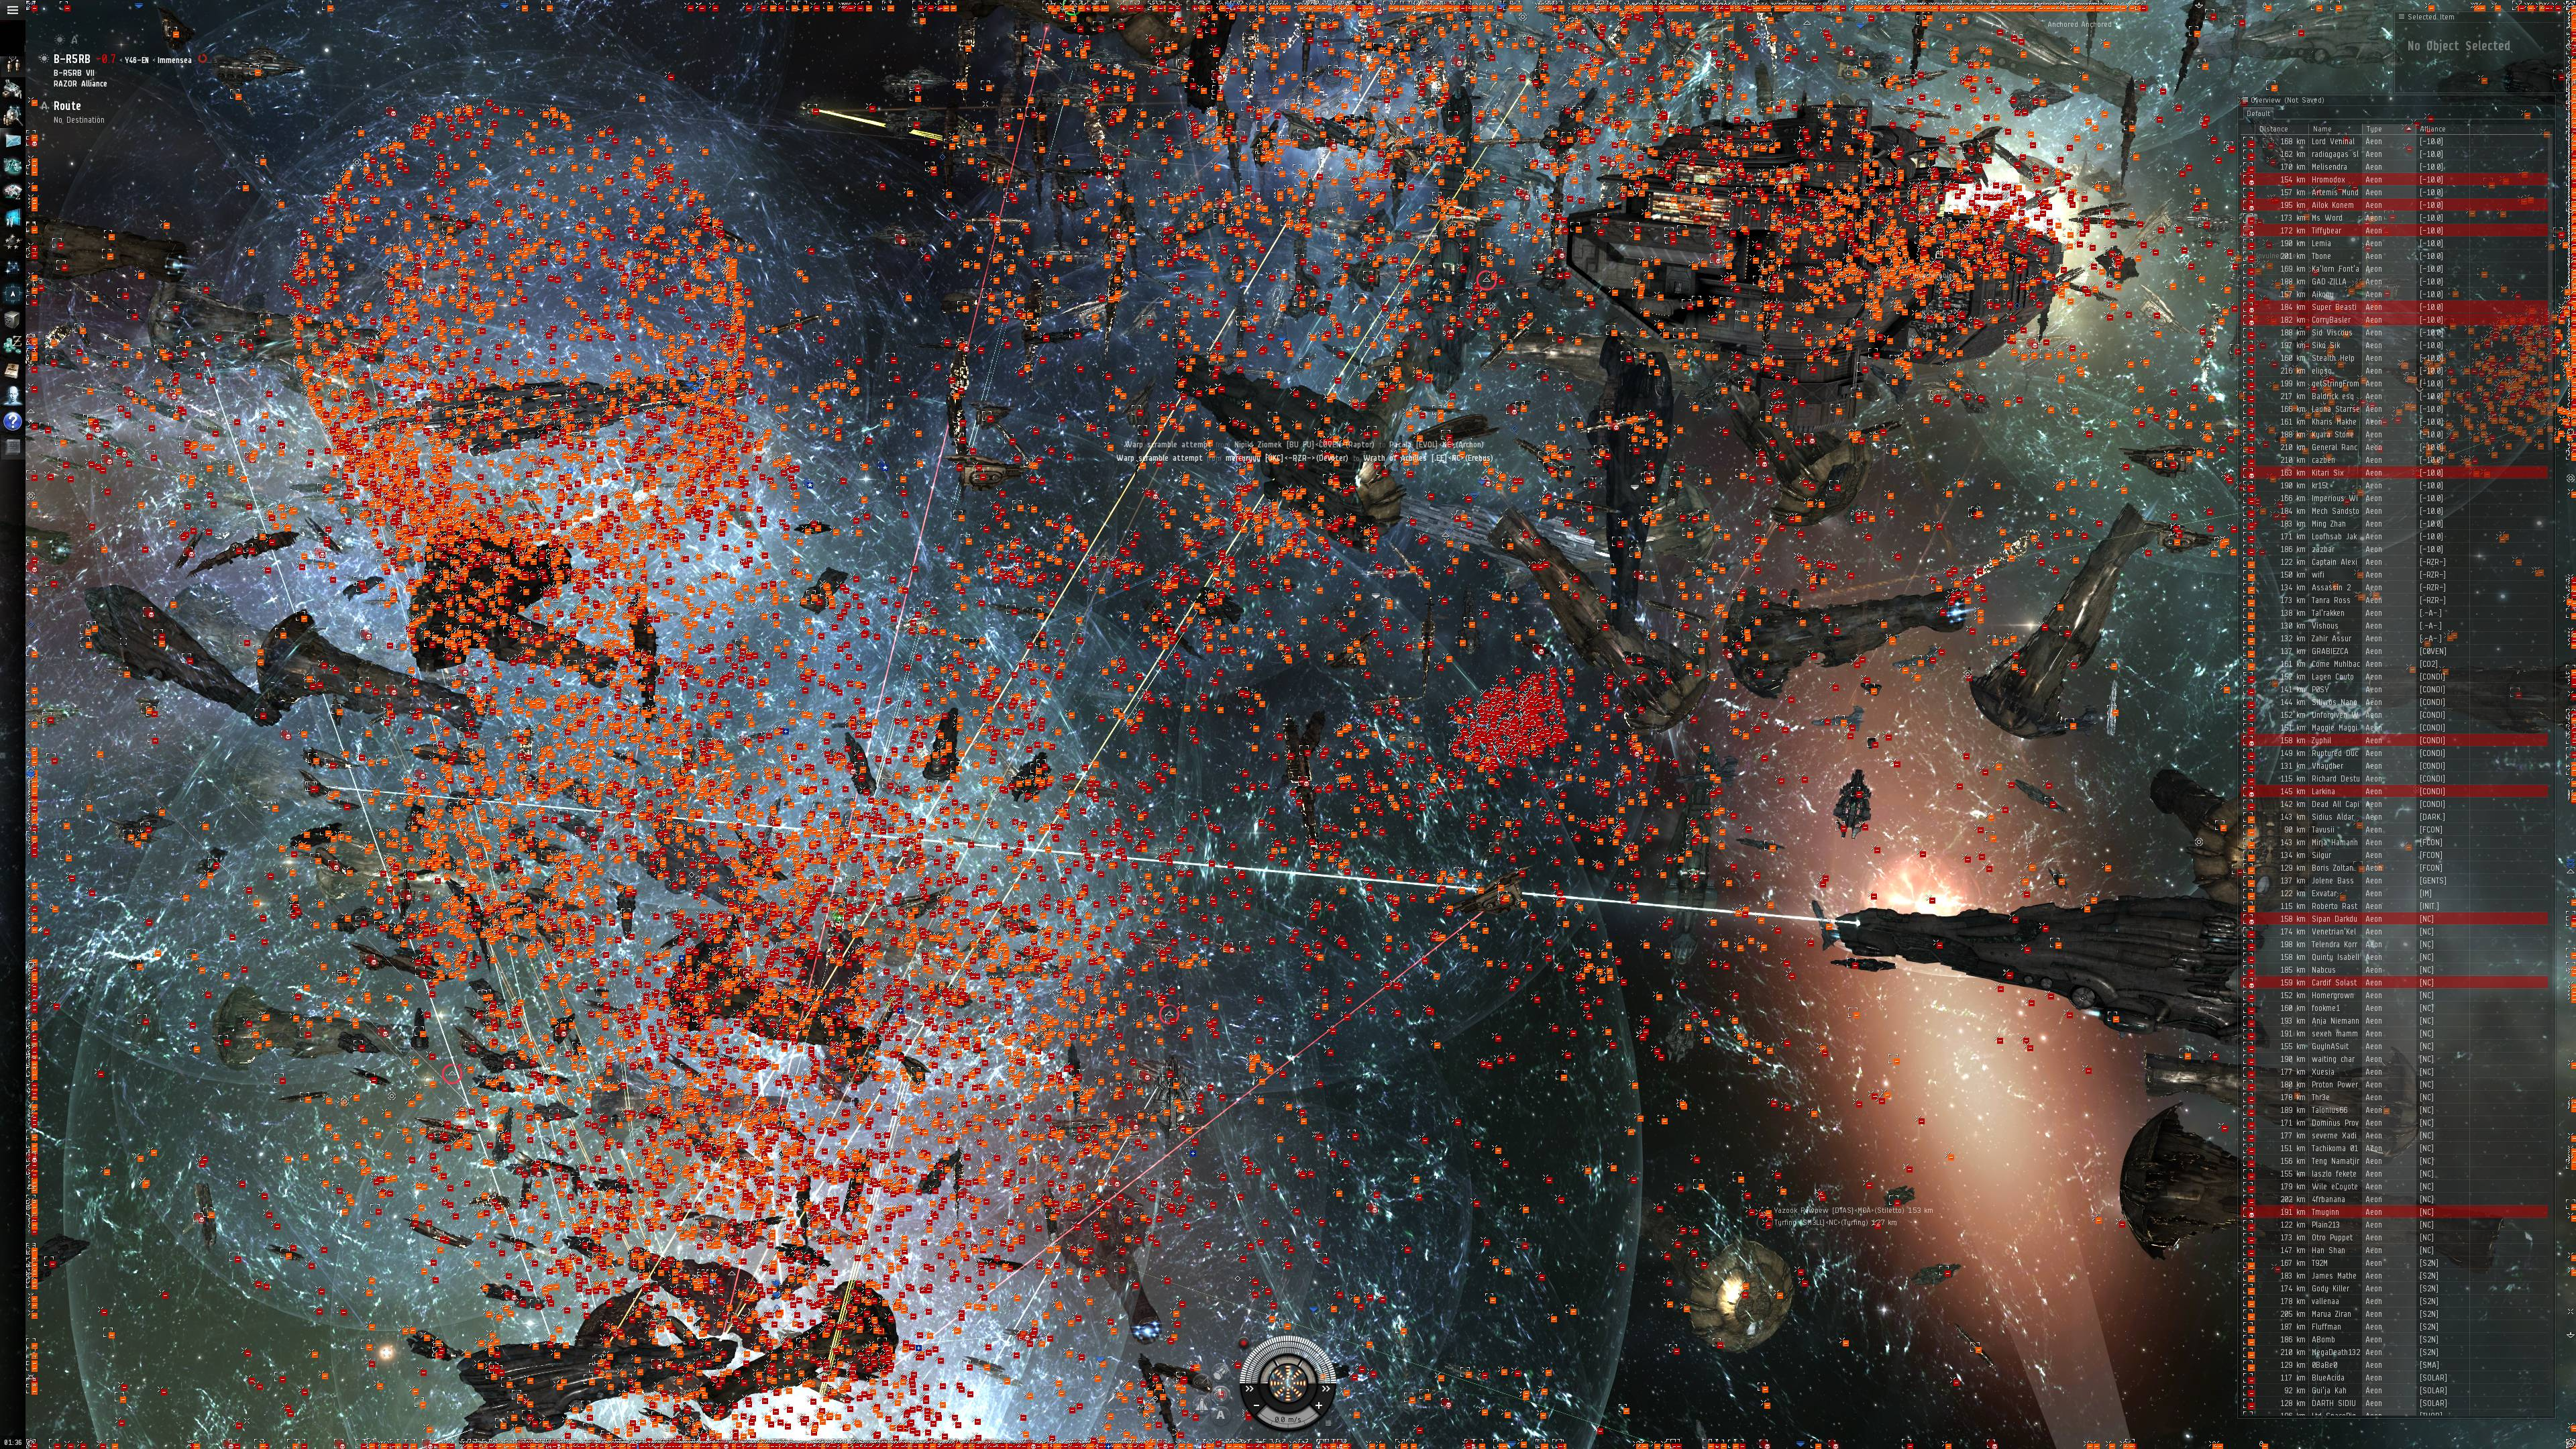
\includegraphics[width=\textwidth]{figures/ch1/eveonline}
			\caption[Énorme bataille dans le jeu \emph{EVE Online}]{Énorme bataille dans le jeu \emph{EVE Online}. Le nombre précis d'unités est inconnu, mais chaque point rouge ou orange représente un vaisseau ou un drone, donc une cible potentielle. Crédit : \emph{EVE Online Community} ; développé et édité par CCP Games.}
			\label{fig:eveonline}
		\end{subfigure}
		\caption[Jeux de stratégie]{Jeux de stratégie.}
		\label{fig:stratGames}
	\end{figure}
	
	\subsection{Arènes de bataaille en ligne multijoueur (MOBA)}
	
	\begin{figure}[!htbp]
		%\centering
		\begin{subfigure}[t]{0.52\textwidth}
			\centering
			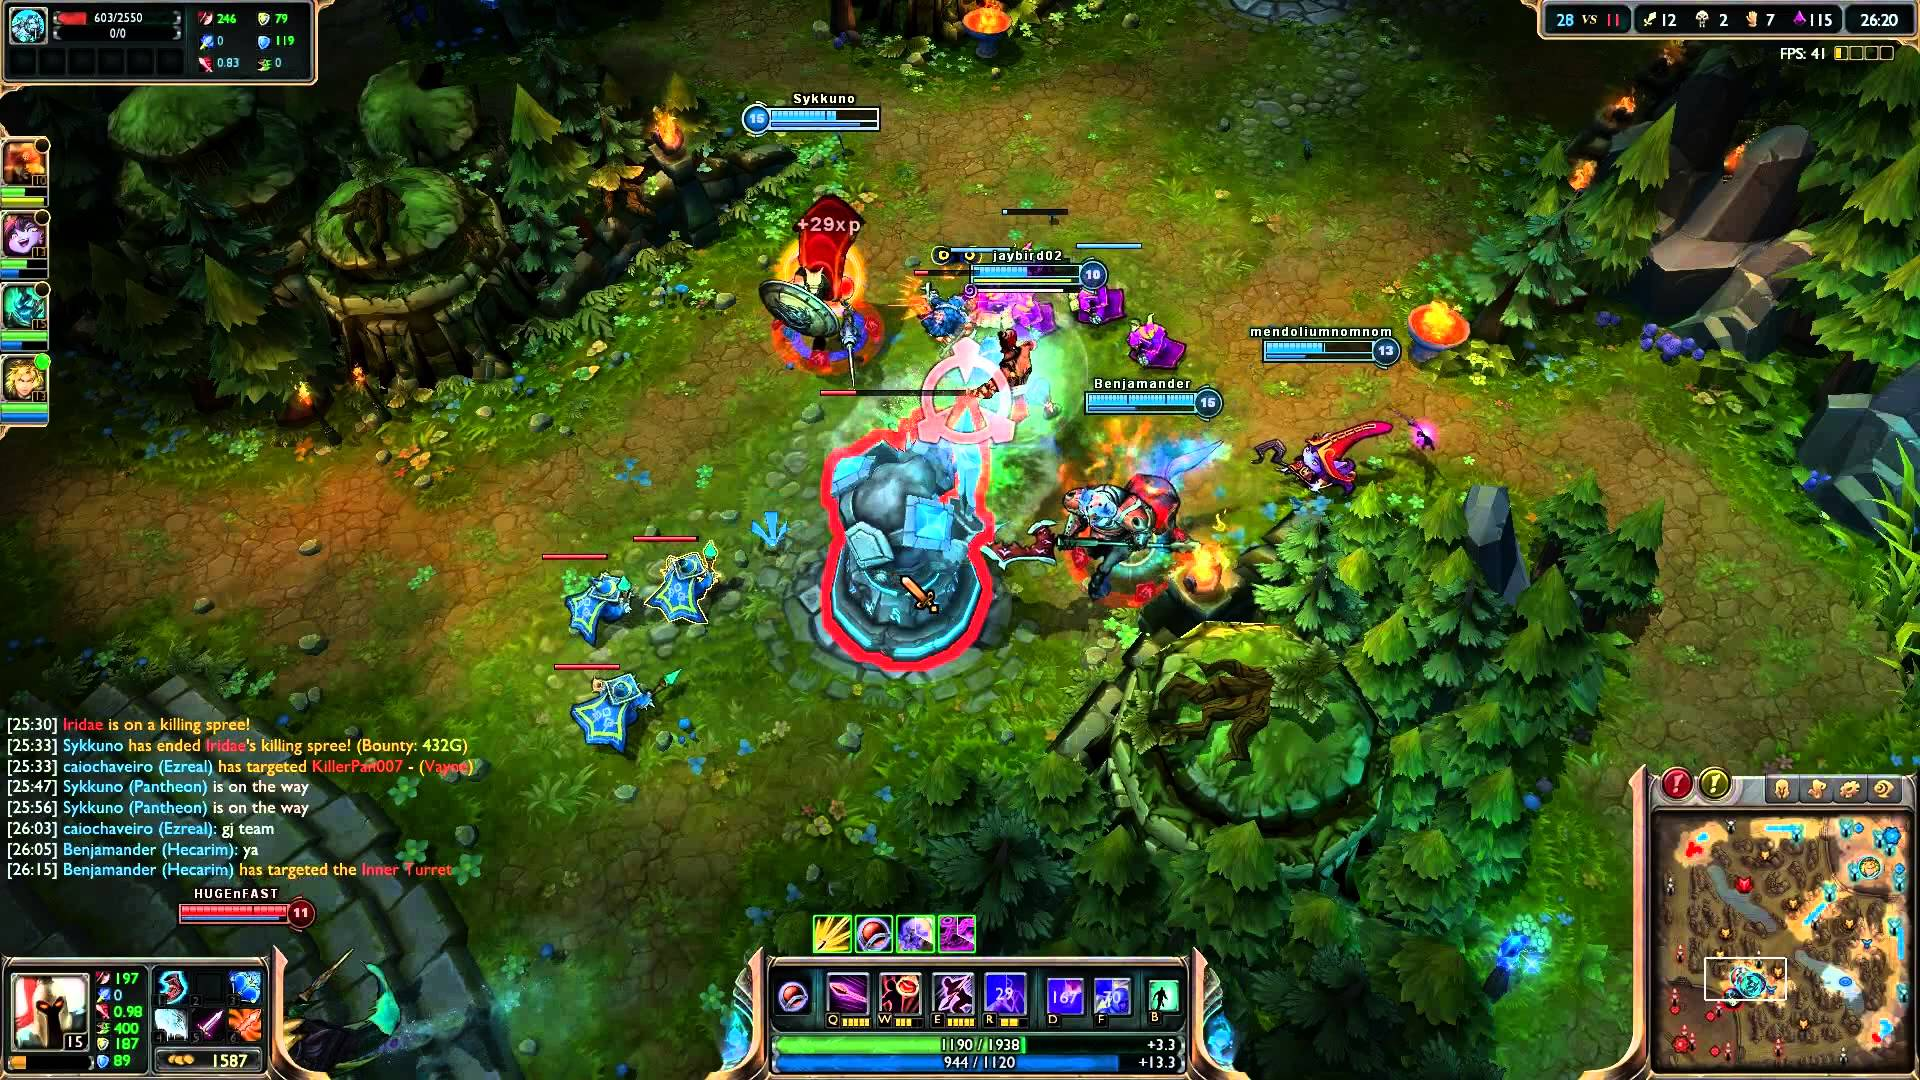
\includegraphics[width=\textwidth]{figures/ch1/lol}
			\caption[Une partie du MOBA \emph{League of Legends}]{\emph{League of Legends}, de Riot Games.}
			\label{fig:lol}
		\end{subfigure}
		~
		\begin{subfigure}[t]{0.46\textwidth}
			\centering
			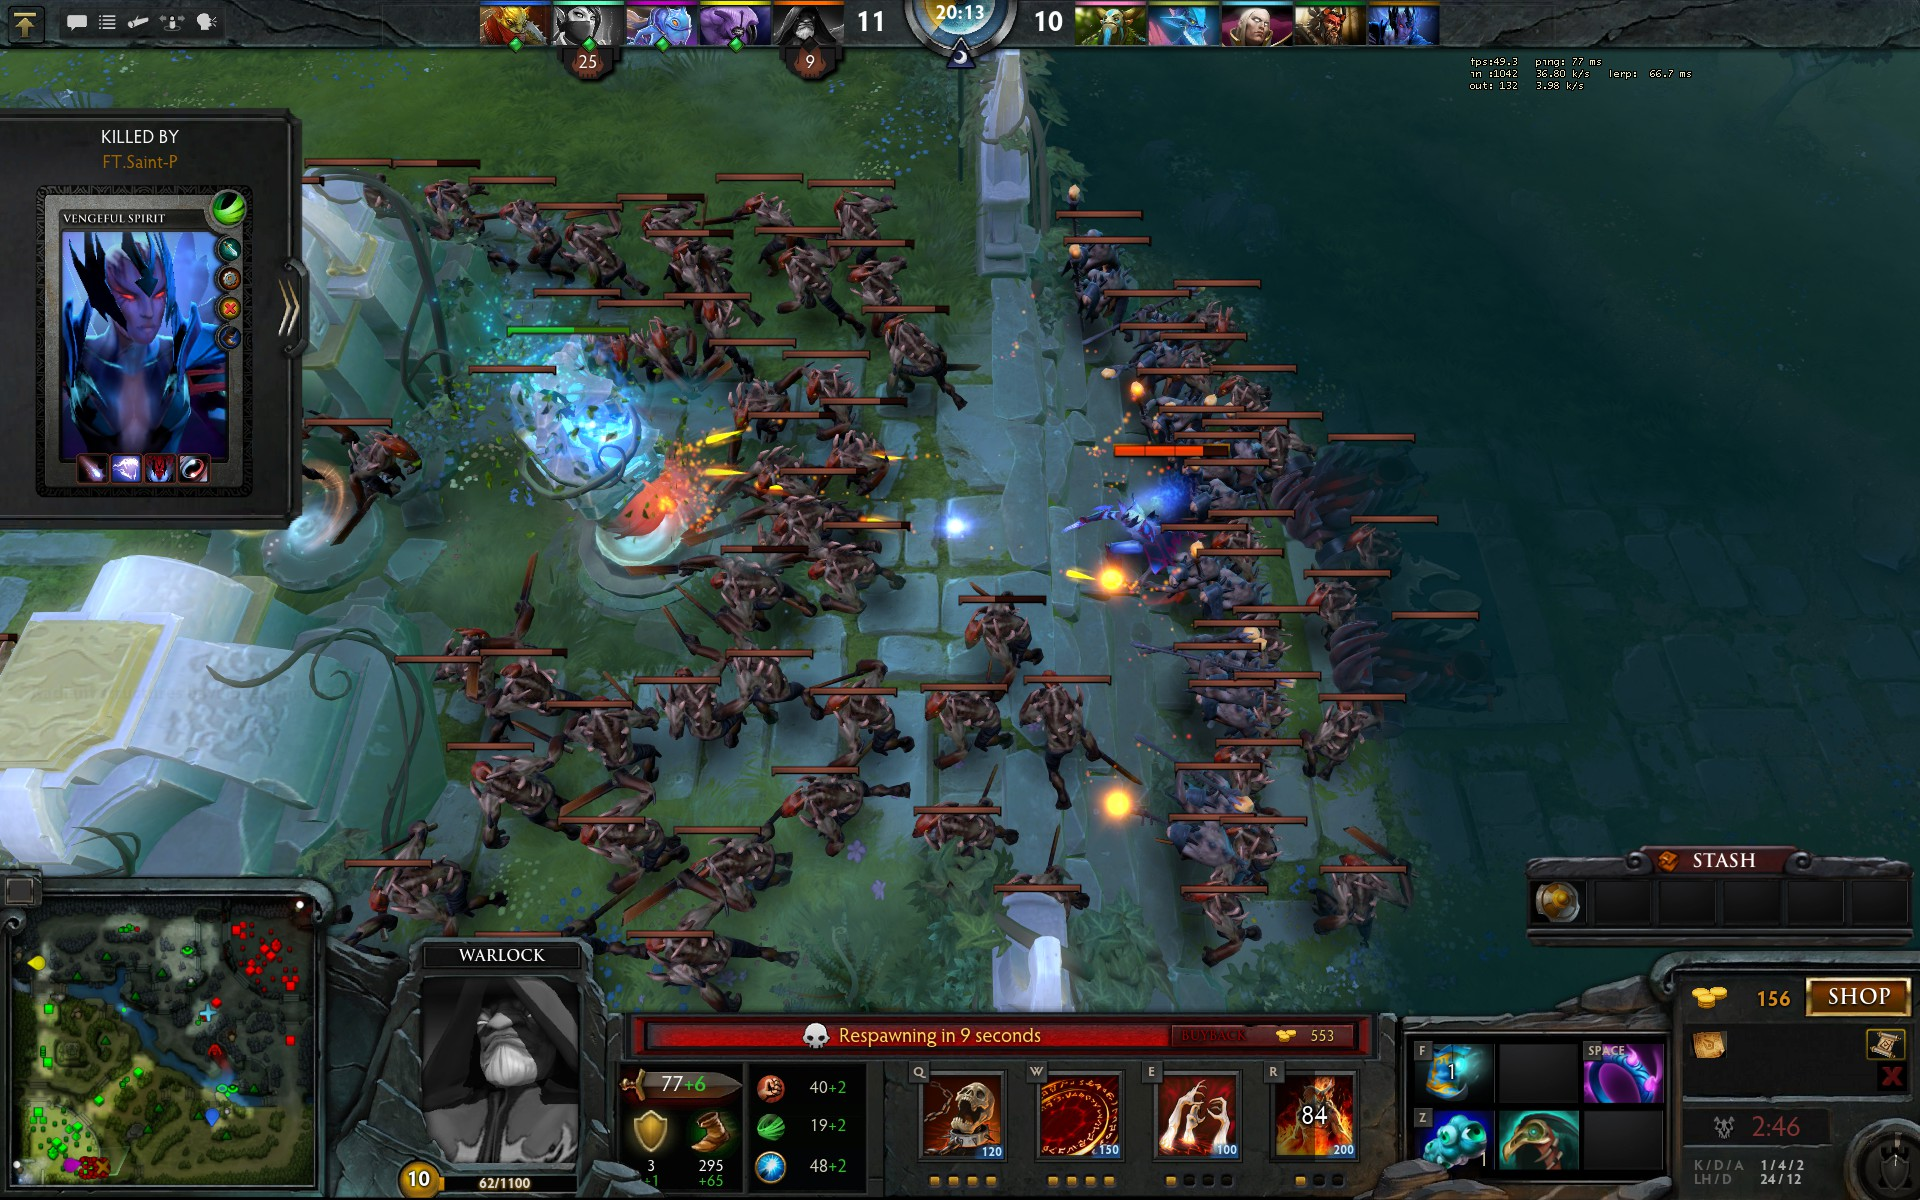
\includegraphics[width=\textwidth]{figures/ch1/dota2}
			\caption[Une partie d'un MOBA, \emph{DOTA~2}]{\emph{DOTA~2}, de Valve Corporation.}
			\label{fig:dota2}
		\end{subfigure}
		\label{fig:mobas}
		\caption[Arènes de bataille en ligne multijoueur (MOBA)]{Arènes de bataille en ligne multijoueur (MOBA). Les objets sont peu nombreux, mais leurs mouvements sont vifs, imprévisibles, et divers événements peuvent créer des effets visuels occultant une partie de l'écran. Pour autant, le jeu ne s'arrête pas pendant ces moments-là et il demeure nécessaire de pouvoir sélectionner des personnages.}
	\end{figure}
	
	
	
	\newcommand{\newrow}{\bigstrut[t] \\ \hline}
	\newcolumntype{Y}{>{\small}X}
	\newcolumntype{Z}{>{\centering}X}
	\begin{table}[!htbp]
		\centering
		\begin{tabularx}{\textwidth}{ Y X X X } % Putain j'entrave que dalle mais ça marche à peu près
		Héros				&	Temps de demi-tour (s)	&	Vitesse (u.a.)	&	Vitesse affichée (cm/s)	\newrow
		Lifestealer			&	0.094 s					&	315				&	63						\newrow
		Shadow Fiend		&	0.094 s					&	315				&	63						\newrow
		Magnus				&	0.118 s					&	315				&	63						\newrow
		Luna				&	0.157 s					&	335				&	67						\newrow
		Keeper of the Light	&	0.188 s					&	335				&	67						\newrow
		Pugna				&	0.188 s					&	330				&	66						\newrow
		Enchantress			&	0.236 s					&	335				&	67						\newrow
		\og Maximum \fg{}	&	---						&	550				&	110						\newrow
		\end{tabularx}
		\caption[Caractéristiques de mouvement des personnages vifs de \emph{Dota~2}]{Caractéristiques de mouvement des personnages les plus vifs de \emph{Dota~2}. Les plus \og agiles \fg{} peuvent effectuer un demi-tour en moins de 0,1~s, soit une fréquence d'un peu plus de 10~Hz, ou 20~Hz pour des virages de 90\textdegree, 30~Hz pour 60\textdegree, etc. Les vitesses des personnages sont notées dans les unités arbitraires du jeu (u.a.), et en cm/s telles qu'elles apparaissent sur un écran (en supposant un écran de bureau de taille et de définition courantes). La ligne \emph{Maximum} correspond à la vitesse \og maximale \fg{} d'un personnage --- en pratique, des objets ou capacités accessibles à certains personnages leur permettent d'aller encore plus vite.}
		\label{tab:dotamoves}
	\end{table}
	% On peut considérer que 128 unités représentent à peu près un mètre dans l'espace virtuel, et apparemment 600 unités feraient environ 12 cm à l'écran, soit environ 2 mm par unité.
	% https://www.hiveworkshop.com/threads/warcraft-iii-distance-units-convert.137848/
	% https://www.reddit.com/r/DotA2/comments/1vaklc/how_big_is_the_dota2_map_really/
	
	
	
	
	


	\subsection{Richesse et diversité}
	
	\begin{figure}[!htbp]
		\centering
		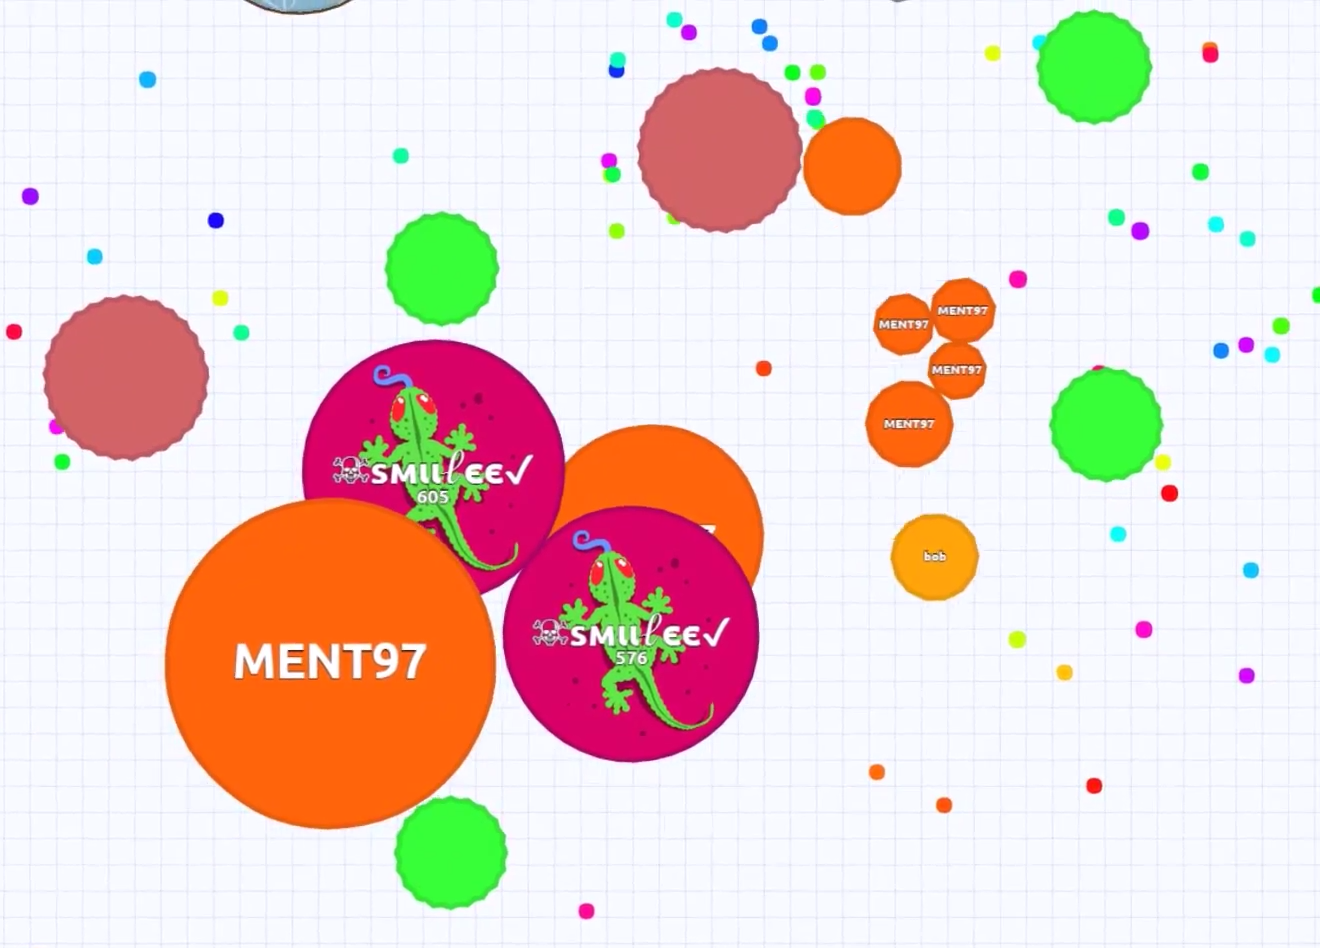
\includegraphics[width=0.6\textwidth]{figures/ch1/agario}
		\caption[\emph{Agar.io}]{\emph{Agar.io} : chaque ensemble de disques d'un même nom est contrôlé par un joueur, et doit dévorer les autres. Ceux à bords dentés sont de dangereux obstacles. Chaque petit disque sans texte est de la nourriture à attraper. Les cibles sont nombreuses et leur agancement est complexe, d'autant qu'elles sont contrôlées par des humains qui cherchent à s'abriter derrière les obstacles. Développé et édité par Matheus Valadares.}
		\label{fig:agario}
	\end{figure}
	
	%	\footnotetext{\url{https://www.youtube.com/watch?v=XaZ2n_feTko}}


\cleardoublepage

\FloatBarrier
\chapter{Séléction de cibles : état de l'art}
\minitoc
\label{appendix:annexeC}

\section{Modèles théoriques pour la sélection de cibles}
	\begin{figure}[!htbp]
		\centering
		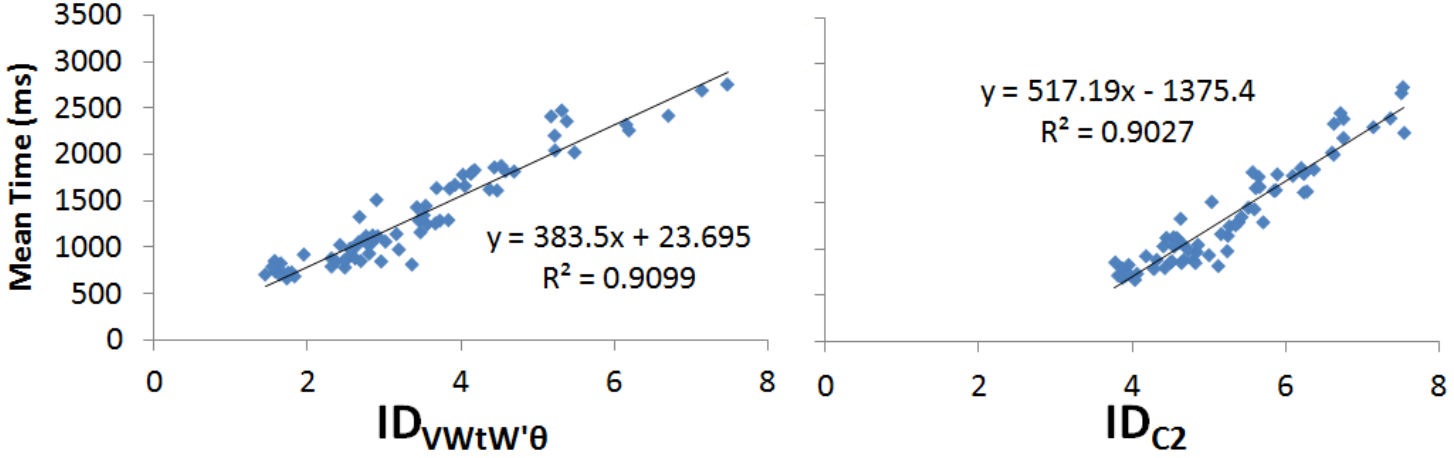
\includegraphics[width=\textwidth]{figures/ch2/holdID}
		\caption[ID vs. nature du mouvement et temps de sélection]{Temps de sélection en fonction des indices de difficulté développés par Al Harji \emph{et al.} Les deux indices sont très fortement corrélés avec les temps de sélection mesurés (sans aucune assistance à la sélection). Crédit : \cite{hajri2011moving}.}
		\label{fig:holdID}
	\end{figure}


\section{Curseurs zonaux}
	\subsection{\emph{Prince}}
	\label{sub:prince}
	La technique \emph{Prince}~\cite{kabbash1995prince} consiste à utiliser un rectangle comme curseur de sélection. Les auteurs ont notamment répliqué la fameuse expérience de Fitts en l'inversant : au lieu d'un point comme curseur et de cibles \og larges \fg{} , ils optèrent pour un curseur large et des cibles ponctuelles, comme l'illustre la figure~\ref{fig:princeCursor}.
	
	\begin{figure}[!htbp]
		\begin{subfigure}[t]{0.56\textwidth}
			\centering
			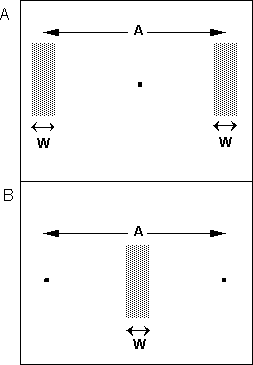
\includegraphics[width=\textwidth]{figures/ch2/princeCursor}
			\caption{À gauche, une représentation schématique de l'expérience de Fitts~\cite{fitts1954information} : un curseur ponctuel est déplacé pour atteindre deux cibles d'aire non nulle. À droite, l'expérience analogue menée dans~\cite{kabbash1995prince}, où le curseur est zonal et les cibles sont ponctuelles.}
			\label{fig:princeCursor}
		\end{subfigure}
		~
		\begin{subfigure}[t]{0.42\textwidth}
			\centering
			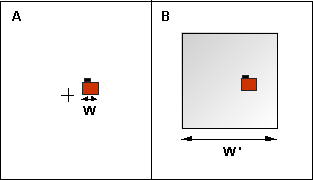
\includegraphics[width=\textwidth]{figures/ch2/princeSelection}
			\caption{Application de la technique \emph{Prince} (à droite) à un cas de sélection pratique, avec pour cible une icône d'aire non nulle ; à gauche, un curseur classique est utilisé.}
			\label{fig:princeSelection}
		\end{subfigure}
		\caption[\emph{Prince}, curseur et sélection]{Crédit : \cite{kabbash1995prince}.}
		\label{fig:princeCursorSelection}
	\end{figure}

	Les auteurs ont pu constater que la loi de Fitts s'appliquait bien à cette configuration, de fait sensiblement identique à celle évaluée par Fitts. Naturellement, dans un environnement de bureau classique, les cibles ne sont pas ponctuelles, mais généralement des icônes ou des boutons d'aire non nulle, comme sur la figure~\ref{fig:princeSelection}, et ce quel que soit le curseur utilisé. De fait, en utilisant un curseur de largeur $W'$, c'est $W'$ qui détermine la difficulté de sélection et non plus la largeur $W$ de la cible (si $W' > w$). Avec un curseur suffisamment gros, l'indice de difficulté peut être considérablement réduit.
	
	La technique \emph{Prince} présente également l'avantage de permettre la sélection de plusieurs cibles d'un coup si elles sont incluses dans le curseur, mais cet avantage reflète une limitation de \emph{Prince}, car il peut dans ces cas-là y avoir ambiguïté si l'utilisateur ne souhaite sélectionner qu'une seule cible.
	
	\subsection{\emph{(Sticky) Area Cursor}, \emph{stickiness} et adaptativité}
	\label{sub:areaCursor}
	Une solution à ce problème d'ambiguïté est proposée par Worden \emph{et al.}~\cite{worden1997making} : lorsqu'un curseur zonal recouvre plusieurs cibles, le curseur devient en pratique un curseur ponctuel, et seul son centre est actif, comme l'illustre la figure~\ref{fig:areaCursor}.
	
	\begin{figure}[!htbp]
		\centering
		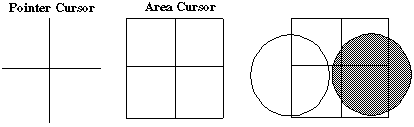
\includegraphics[width=0.70\textwidth]{figures/ch2/areaCursor}
		\caption[\emph{Area Cursor} avec \emph{hot spot}]{Un curseur zonal dont seul le centre, marqué par l'intersection de deux segments, demeure actif lorsque le curseur chevauche plusieurs cibles. Crédit : \cite{worden1997making}.}
		\label{fig:areaCursor}
	\end{figure}
	
	Cette technique simple permet de tirer parti des avantages d'un curseur zonal quand la densité de cibles est suffisamment faibles, sans pour autant souffrir de ses inconvénients lorsqu'elle est élevée, puisque l'on revient alors à un simple curseur ponctuel.
	
	\paragraph{\emph{Stickiness}.}
	À cette solution, Worden \emph{et al.} ont ajouté l'usage de \emph{stickiness} adaptative pour les icônes. Un curseur est dit \emph{sticky} si, lorsqu'il s'approche d'une icône, celle-ci devient \og collante \fg{}. En pratique, le ratio de sensibilité du curseur (la quantité du curseur par rapport à la quantité de mouvement du périphérique de saisie) diminue, ce qui permet d'une part de ralentir le curseur automatiquement, et d'autre part d'affiner les mouvements correctifs permettant la sélection d'une cible lors de son approche.
	
	Le problème des cibles collantes est que lorsque leur densité est élevée, donc en présence de nombreux distracteurs, la trajectoire du curseur se trouve fortement perturbée par ceux-ci, ce qui peut être contre-productif, ou du moins limiter les bénéfices de cette technique. La solution proposée par Worden \emph{et al.} est de ne rendre les cibles collantes que lorsque le curseur est à moins de 30~\%{} de la vitesse maximale qu'il a atteinte au cours de la tâche de sélection courante. L'hypothèse est qu'une sélection commence par une phase de mouvement très rapide et ample, suivie de petits mouvements correctifs plus lents, et que le curseur sera donc relativement lent près de la cible réellement visée par l'utilisateur.
	
	L'\emph{Area cursor}, en particulier complémenté par des cibles collantes et un gain adaptatif, permet un gain de performances important, en particulier avec des utilisateurs âgés, comme le détaille le tableau~\ref{tab:areaCursor}.
	
	\begin{table}
	\centering
	\begin{tabular}{l c c c c}
										& \multicolumn{2}{c}{Jeunes}	&	\multicolumn{2}{c}{Âgés}			\\
										& Temps (ms)	& Taux de succès	& Temps (ms)	& Taux de succès	\\
		Pointeur seul					& 759			& 95,0				& 1893			& 95,0				\\
		Pointeur collant				& 712			& 97,4				& 1869			& 96,3				\\
		Pointeur adaptatif				& 743			& 97,7				& 1485			& 95,5				\\
		\emph{Area cursor} seul			& 639			& 96,9				& 1658			& 96,3				\\
		\emph{Area cursor} collant		& 596			& 97,9				& 1596			& 97,7				\\
		\emph{Area cursor} adaptatif	& 591			& 99,0				& 1203			& 97,9				\\
	\end{tabular}
	\caption[\emph{Area cursor} -- performances]{\emph{Area cursor} : performances mesurées pour des cibles collantes, avec et sans gain adaptatif en fonction de la vitesse du curseur. Les résultats sont comparés avec un curseur ponctuel dans les mêmes conditions, avec des sujets jeunes (23,4 ans en moyenne) et plus âgés (70,1 ans en moyenne). Les performances sont rapportées par le temps de sélection ainsi que le taux de succès (pourcentage de sélections réussies). Le curseur zonal avec cibles collantes et gain adaptatif permet les meilleures performances, surtout avec des sujets âgés. Données tirées de~\cite{worden1997making}.}
	\label{tab:areaCursor}
	\end{table}

	\subsection{\emph{Silk Cursor}}
	\label{sub:silkCursor}
	Le \emph{Silk Cursor}~\cite{zhai1994silk} est analogue aux curseurs zonaux décrits plus haut, mais étendu à la 3D. Il s'agit donc d'un volume semi-transparent que l'utilisateur peut utiliser pour sélectionner un objet en déplaçant le volume de telle sorte que l'objet soit dedans.
	
	Tel qu'il fut évalué dans~\cite{zhai1994silk}, le \emph{Silk Cursor} doit entièrement englober un objet pour pouvoir le sélectionner ; ainsi, dans l'illustration de la figure~\ref{fig:silk}, le poisson ne peut pas encore être sélectionné. Celui-ci était animé par une combinaison de fonctions sinusoïdales agissant indépendamment sur chacune de ses coordonnées (x,y,z). Ces fonctions sont détaillées par les équations~\ref{eq:silkMotion0}, \ref{eq:silkMotion1} et~\ref{eq:silkMotion2} où $t$ est le temps, $A = 4,55$~cm, $p = 2$, $f_{0} = 0,02$~Hz, 	$\phi_{x}(i)$, $\phi_{y}(i)$ et $\phi_{z}(i)$ sont des nombres pseudo-aléatoires, échantillonés uniformément entre $0$ et $2\pi$. Ces fonctions ont pour but de produire un mouvement lisse (\emph{smooth}) et subjectivement imprévisible~\cite{zhai1993human}.
	
	\begin{align}
		\label{eq:silkMotion0}
		x(t) &= \sum_{i=0}^{5} Ap^{-i} \sin \left( 2\pi{}f_{0}p^{i}t + \phi_{x}(i) \right) \\
		\label{eq:silkMotion1}
		y(t) &= \sum_{i=0}^{5} Ap^{-i} \sin \left( 2\pi{}f_{0}p^{i}t + \phi_{y}(i) \right) \\
		\label{eq:silkMotion2}
		z(t) &= \sum_{i=0}^{5} Ap^{-i} \sin \left( 2\pi{}f_{0}p^{i}t + \phi_{z}(i) \right) - 7.8
	\end{align}
	
	\subsection{Temps de sélection}
	Les performances du \emph{Silk Cursor} furent évaluées par Zhai \emph{et al.} en le comparant à un curseur volumique de fonctionnement identique, mais rendu en fil de fer, dans des conditions monoscopiques et stéréoscopiques (voir la figure~\ref{fig:silkPerf}). Comme le supposaient les auteurs, la semi-transparence du curseur permet une forte amélioration du temps de sélection, particulièrement avec un écran monoscopique. De plus, la stéréoscopie réduit le temps de sélection de façon significative, et ce même avec le \emph{Silk Cursor}.
	
	\begin{figure}[!htbp]
		\begin{subfigure}[t]{0.42\textwidth}
			\centering
			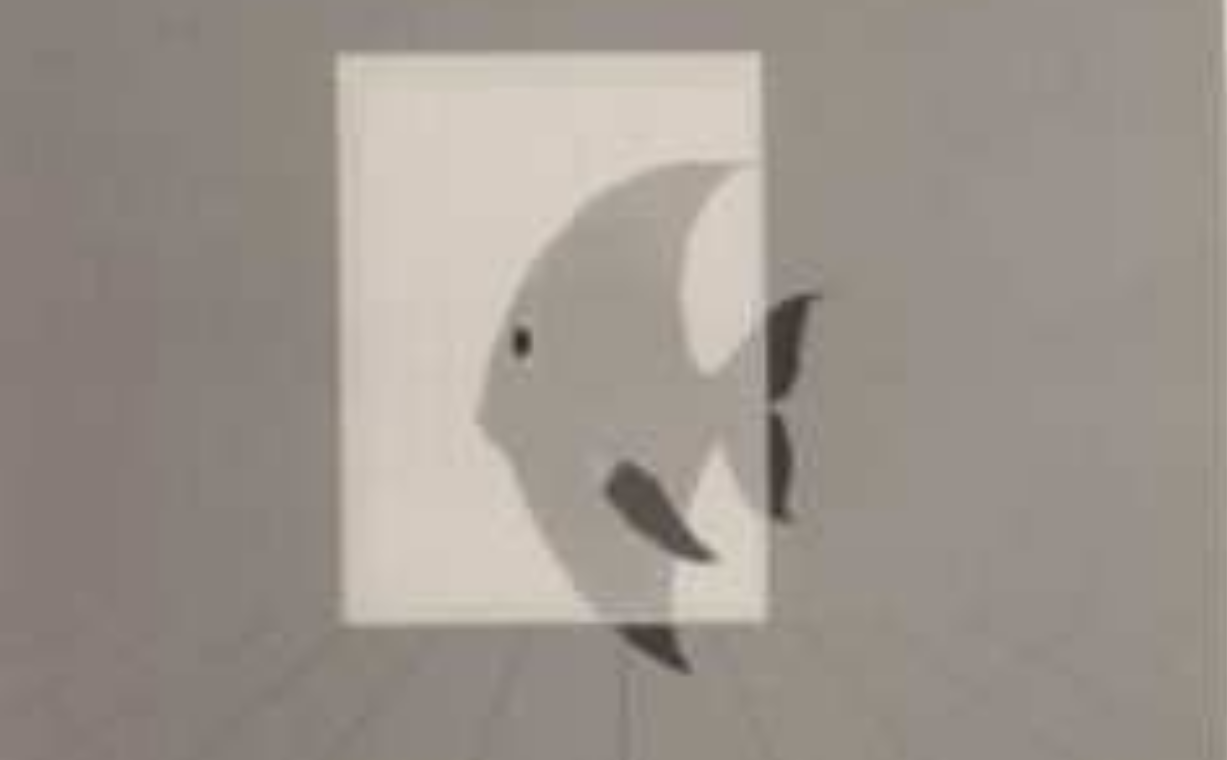
\includegraphics[width=\textwidth]{figures/ch2/silk}
			\caption{Le \emph{Silk Cursor} : l'utilisateur est ici en train d'essayer de sélectionner un poisson, en l'englobant avec le volume du curseur. Quelques parties du poisson ne sont pas incluses dans le volume de sélection, et de fait il ne peut pas encore être sélectionné.}
			\label{fig:silk}
		\end{subfigure}
		~
		\begin{subfigure}[t]{0.56\textwidth}
			\centering
			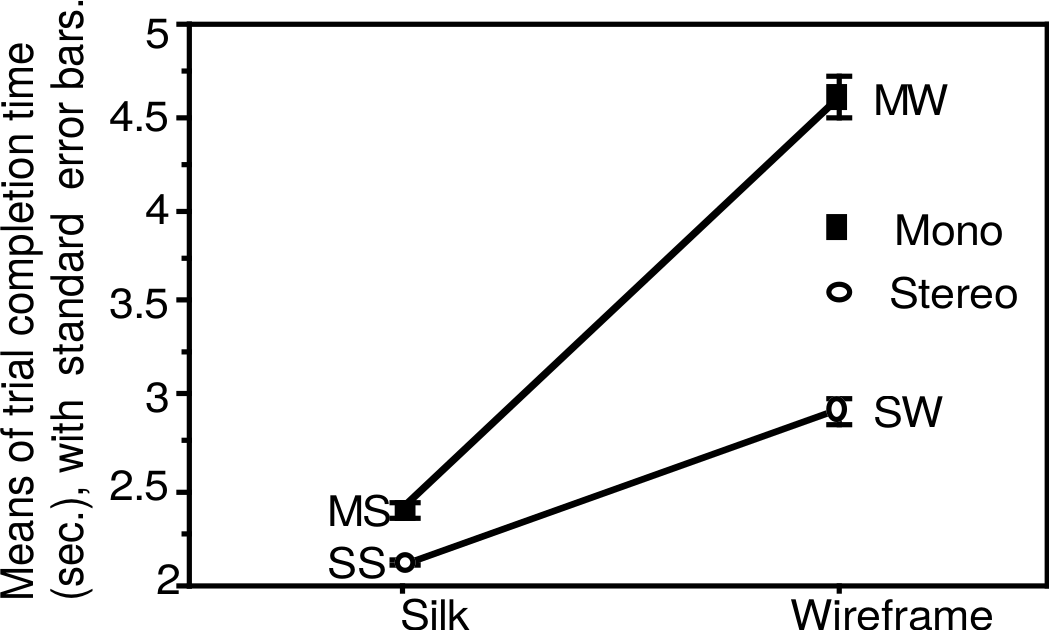
\includegraphics[width=\textwidth]{figures/ch2/silkPerf}
			\caption{Temps de sélection du \emph{Silk Cursor} et d'un curseur volumique en fil de fer. Première lettre : \emph{M} $\rightarrow$ condition monoscopique ; \emph{S} $\rightarrow$ condition stéréoscopique. Seconde lettre : \emph{S} $\rightarrow$ \emph{Silk Cursor} ; \emph{W} $\rightarrow$ curseur en fil de fer (\emph{wireframe}). La stéréoscopie et le \emph{Silk Cursor} améliorent fortement les performances.}
			\label{fig:silkPerf}
		\end{subfigure}
		\caption[\emph{Silk Cursor}]{\emph{Silk Cursor}. Crédit : \cite{zhai1994silk}}
		\label{fig:silkCursorPerf}
	\end{figure}
	
	Observons toutefois que la conception de l'évaluation pourrait favoriser ce dernier de façon artificielle, en ce qu'il est nécessaire que l'objet visé soit intégralement inclus dans le curseur volumique, ce qui ne paraît pas indispensable dans l'absolu. Or, en fil de fer, vérifier cela visuellement est très difficile, tandis que s'assurer qu'une partie de l'objet est dans le curseur semble plus aisé. On peut supposer que la différence de difficulté entre ces deux tâches est moindre avec le \emph{Silk Cursor} grâce aux indications fournies par la semi-transparence, qui facilite la perception de la profondeur et des objets occultés.
	
	\subsection{Taux et amplitude des erreurs}
	Les auteurs ont également évalué les performances du \emph{Silk Cursor} en matière d'erreurs, tant pour leur taux d'occurrence (voir la figure~\ref{fig:silkErrors}) que pour leur amplitude (voir la figure~\ref{fig:silkErrorMag}). Cette technique de sélection permet donc d'améliorer les temps de sélection, de réduire les occurrences d'erreurs et de diminuer leur amplitude lorsqu'elles se produisent malgré tout.
	
	\begin{figure}[!htbp]
		\begin{subfigure}[t]{0.49\textwidth}
			\centering
			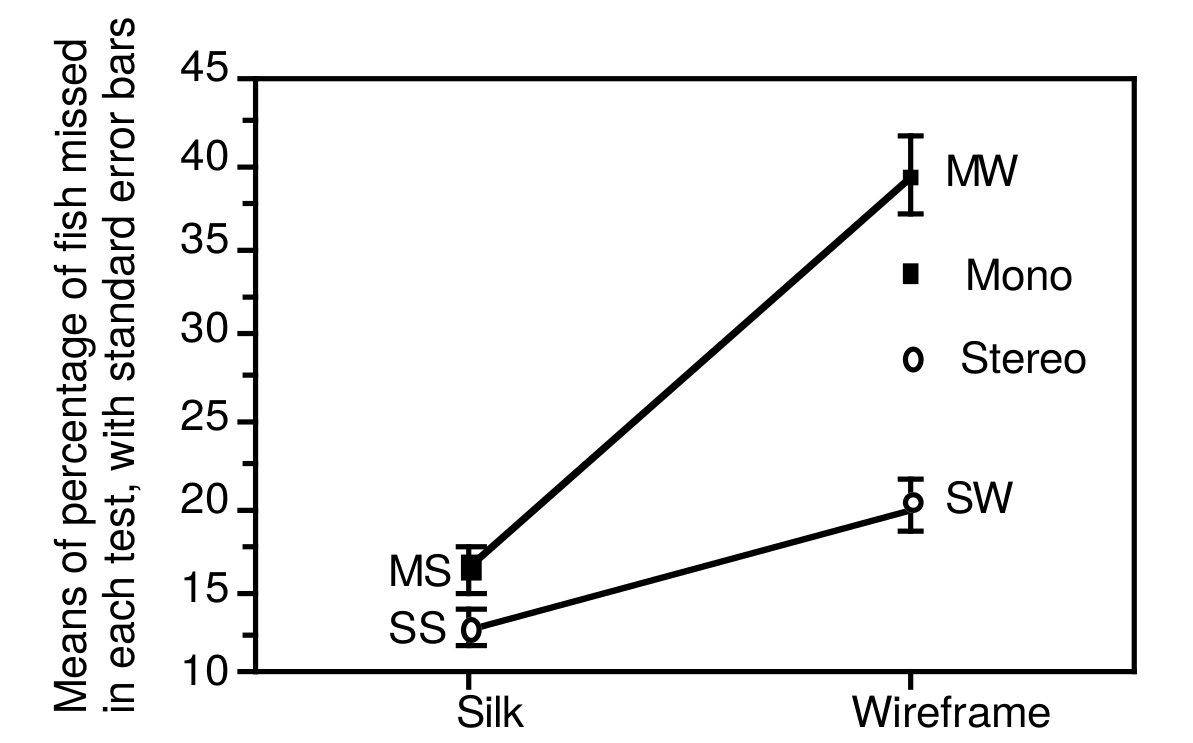
\includegraphics[width=\textwidth]{figures/ch2/silkErrors}
			\caption{Taux d'erreurs du \emph{Silk Cursor} comparé à un curseur volumique. Ici encore, la stéréoscopie et le \emph{Silk Cursor} améliorent les performances.}
			\label{fig:silkErrors}
		\end{subfigure}
		~
		\begin{subfigure}[t]{0.49\textwidth}
			\centering
			\includegraphics[width=\textwidth]{figures/ch2/silkErrorMag}
			\caption{Erreurs : distance euclidienne entre la position du curseur et celle souhaitée pour saisir la cible. La stéréoscopie et le \emph{Silk Cursor} améliorent les performances.}
			\label{fig:silkErrorMag}
		\end{subfigure}
		\caption[\emph{Silk Cursor} -- Occurrences et amplitude des erreurs]{\emph{Silk Cursor} -- erreurs. Crédit : \cite{zhai1994silk}}
		\label{fig:SilkErrorsErrMag}
	\end{figure}
	
	Enfin, cette étude menée par Zhai \emph{et al.}~\cite{zhai1994silk} confirme l'intérêt du rendu stéréoscopique pour de telles tâches, et montre qu'il apporte toujours un bénéfice tangible lorsqu'il est combiné au \emph{Silk Cursor}.
	
	\subsection{Impressions subjectives}
	Zhai \emph{et al.} ont également recueuilli les impressions subjectives des sujets (table~\ref{tab:silkImpr}). Le \emph{Silk Cursor} fut évalué très positivement par les utilisateurs, qui ont même préféré sa version monoscopique à la version stéréoscopique du curseur en fil de fer. En stéréoscopie, toutes les impressions subjectives étaient au moins hautes, et souvent très hautes.

	\begin{table}
	\centering
	\begin{tabular}{c | c c c c c}
							& \multicolumn{5}{c}{Impressions subjectives} \\
		Condition			& Très basse	& Basse	& Moyenne	& Haute	& Très haute \bigstrut[b] \\ \hline
		\emph{MonoWire}		& 8				& 2		& 1			&		& \bigstrut[t]	\\
		\emph{MonoSilk}		& 				& 		& 4			& 4		& 4 			\\
		\emph{StereoWire}	& 				& 2		& 7			& 3		& 	 			\\
		\emph{StereoSilk}	& 				& 		& 			& 3		& 9 			\\
	\end{tabular}
	\caption[\emph{Silk Cursor} -- impressions subjectives]{Impressions subjectives du \emph{Silk Cursor}. Chaque case contient le nombre de sujets ayant évalué la condition correspondante de la sorte. Le \emph{Silk Cursor} s'illustre par les 9 très hautes appréciations reçues en stéréoscopie. Source :~\cite{zhai1994silk}.}
	\label{tab:silkImpr}
	\end{table}





\section{Lancer de rayon avec désambiguïsation}

	\begin{figure}[!htbp]
		\centering
		\includegraphics[width=0.46\textwidth]{figures/ch2/rayFootprint}
		\caption[\emph{Raycasting} et désambiguïsation -- distance parcourue par le périphérique]{Distance parcourue par le périphérique de pointage avec les techniques de \emph{raycasting} évaluées. Les \emph{Depth, Lock} et \emph{Flower Rays} font mieux que le curseur ponctuel, au contraire du \emph{Smart Ray} qui affiche en sus un écart-type considérable. Crédit : \cite{grossman2006design}.}
		\label{fig:rayFootprint}
	\end{figure}



















\FloatBarrier
\section{Techniques de sélection en cascade}

	\subsection{\emph{Look \&{} Touch}}

	\begin{figure}[!htbp]
%		\centering
		\begin{subfigure}[t]{\textwidth}
			\centering
			\includegraphics[width=\textwidth]{figures/ch2/latRes}
			\caption[\emph{Look \&{} Touch} -- performances]{Performances. Les temps de sélection sont en haut, et les taux d'erreurs en bas. Les mentions $S_{i}$ et $D_{i}$ indiquent respectivement les différentes tailles et distances.}
			\label{fig:latRes}
		\end{subfigure}
		~
		\begin{subfigure}[t]{\textwidth}
			\centering
			\includegraphics[width=\textwidth]{figures/ch2/latSubj}
			\caption[\emph{Look \&{} Touch} -- impressions subjectives]{Impressions subjectives recueillies par Stellmach \emph{et al.} auprès des sujets de l'évaluation. La technique \emph{MAGIC tab} l'emporte, mais d'une très courte tête.}
			\label{fig:latSubj}
		\end{subfigure}
		\caption[\emph{Look \&{} Touch} -- performances]{\emph{Look \&{} Touch} -- performances et impressions. Crédit : \cite{stellmach2012look}.}
	\end{figure}
	
	
	
	
	\subsubsection{\emph{Sphere-casting refined by QUAD-menu
(SQUAD)}}
	
	
	\begin{figure}[!htbp]
		\centering
		\includegraphics[width=\textwidth]{figures/ch2/squad}
		\caption[Fonctionnement de la technique SQUAD]{SQUAD : à gauche, la première étape de sélection, au cours de laquelle l'utilisateur pré-sélectionne une portion de l'espace à l'aide d'une sphère. À droite, la phase suivante, permettant d'affiner la sélection. Les objets pré-sélectionnés avec la sphère sont uniformément répartis dans quatre quadrants d'un menu, et l'utilisateur n'a plus qu'à choisir le quadrant contenant l'objet qu'il souhaite sélectionner. Les autres quadrants se vident, puis les objets du quadrant sélectionné sont répartis dans les quatre afin de permettre, dans une nouvelle étape, d'affiner encore la sélection. L'opération est répétée jusqu'à ce qu'il n'y ait plus qu'un objet, qui est sélectionné. Crédit : \cite{kopper2011rapid}.}
		\label{fig:squad}
	\end{figure}
	
	
	
	
	\begin{figure}[!htbp]
		\centering
		\includegraphics[width=\textwidth]{figures/ch2/squad2}
		\caption[La technique SQUAD -- évaluation]{SQUAD tel qu'évalué dans~\cite{kopper2011rapid}. Dans la première phase (à gauche) les petites sphères sont réparties sur la surface d'une grande sphère invisible centrée sur l'utilisateur, de sorte qu'elles sont toutes à la même distance de lui, afin qu'elles aient toutes une taille apparente égale une fois projetées sur l'écran. La cible à saisir est identifiée par sa couleur rouge. Seule l'orientation du périphérique de pointage était prise en compte dans la première phase, et les sujets avaient pour consigne de maintenir sa position dans une zone déterminée. Crédit : \cite{kopper2011rapid}.}
		\label{fig:squad2}
	\end{figure}
	


	\begin{figure}[!htbp]
		\centering
		\includegraphics[width=0.7\textwidth]{figures/ch2/squadRecap}
		\caption[SQUAD : erformances et taille des cibles.]{Performances en fonction de la taille de la cible. Les performances de SQUAD ne sont pas significativement modifiées par la taille ; celles du \emph{raycasting} le sont fortement. SQUAD brille particulièrement avec de petites cibles, mais se montre désavantageuse quand elles sont grandes. Crédit : \cite{kopper2011rapid}.}
		\label{fig:squadRecap}
	\end{figure}



	
	\subsubsection{\emph{Disambiguation Canvas}}
	
	\begin{figure}[!htbp]
		\centering
		\includegraphics[width=0.80\textwidth]{figures/ch2/dCanvas2}
		\caption[\emph{Disambiguation Canvas}, bis]{Fonctionnement du \emph{Disambiguation Canvas}. En (a), une photo d'un utilisateur de la technique, équipé d'un HMD et d'un pointeur ; en (b), l'espace virtuel utilisé pour évaluer la technique. Comme dans l'évaluation originale de SQUAD, les petites sphères sont réparties sur la surface d'une grande sphère invisible~\cite{kopper2011rapid}, ce qui permet d'uniformiser leurs tailles apparentes. Crédit : \cite{debarba2013disambiguation}.}
		\label{fig:dCanvas2}
	\end{figure}
	
	
	\begin{figure}[!htbp]
		\centering
		\includegraphics[width=0.8\textwidth]{figures/ch2/dCanvasLayout}
		\caption[\emph{Disambiguation Canvas} -- calibrage]{(a) : étape de calibrage pour la deuxième phase du \emph{Disambiguation Canvas}. On demande ici à l'utilisateur de faire le tour de l'écran avec son pouce, en essayant de s'approcher des bords. Il en résulte un motif fermé représentant l'espace que l'utilisateur peut atteindre confortablement. (b) : cet espace est utilisé pour répartir les objets, dont la cible, que l'utilisateur pourra ainsi sélectionner aisément. Par défaut, l'emplacement du le curseur est laissé vide, pour éviter les sélections accidentelles et faciliter l'annulation en cas d'erreur au cours de la première phase. Crédit : \cite{debarba2013disambiguation}.}
		\label{fig:dCanvasLayout}
	\end{figure}
	

	\begin{figure}[!htbp]
		\centering
		\includegraphics[width=0.80\textwidth]{figures/ch2/dCanvasDensity}
		\caption[\emph{Disambiguation Canvas} -- densité]{La difficulté de sélection avec le \emph{Disambiguation Canvas} dépend du nombre d'objets pré-sélectionnés dans la première étape. (a) : 25 objets peuvent être sélectionnés, et sont de fait assez gros ; (b) : ils sont 97, et de taille moyenne ; (c) : ils sont 224 et nettement plus petits. La loi de Fitts nous indique que les cibles seront plus difficiles à sélectionner en environnement dense, du fait de leur taille réduite. Crédit : \cite{debarba2013disambiguation}.}
		\label{fig:dCanvasDensity}
	\end{figure}
	
	
	
	
	\begin{figure}[!htbp]
		\centering
		\includegraphics[width=\textwidth]{figures/ch2/dCanvasContext}
		\caption[\emph{Disambiguation Canvas} -- animation de transition]{Animation pendant la transition entre la phase de pré-sélection du \emph{Disambiguation Canvas} et la phase de disambiguïsation. Les objets sont réarrangés \og en douceur \fg{} ce qui permet à l'utilisateur de suivre la cible des yeux afin de ne pas la perdre, et de préserver, dans une certaine mesure, le contexte spatial. Crédit : \cite{debarba2013disambiguation}.}
		\label{fig:dCanvasContext}
	\end{figure}












\FloatBarrier
\section{Techniques de prédiction de la trajectoire du curseur}

	\subsection{Le \emph{Delphian Desktop}}
	\label{sub:delphian}
	Le \emph{Delphian Desktop}~\cite{asano2005predictive} est une technique de prédiction de la trajectoire du curseur, qui analyse sa position dans le temps pour essayer de déterminer si un pic de vélocité pour le mouvement en cours a été atteint. Il s'inspire d'observations sur les systèmes perceptif et moteur de l'humain, issues de diverses études de psychologie et kinesthésie~\cite{accot2003refining, graham1995pointing, graham1996physical, mackenzie1992extending, mackenzie1994prediction, takagi2002fundamental, walker1993spatial}.
	
	On sait en effet depuis une étude de Walker \emph{et al.}~\cite{walker1993spatial} que la hauteur du pic de vitesse d'un curseur croît avec la distance entre la cible et lui-même, avec un profil typique illustré par la figure~\ref{fig:delphianPeak}.

	\begin{figure}[!htbp]
		\begin{subfigure}[t]{0.44\textwidth}
			\centering
			\includegraphics[width=\textwidth]{figures/ch2/delphianPeak}
			\caption{Vitesse du curseur. Il accélère au cours de la première phase (\emph{Plan time}) puis décélère (\emph{Adjustment time}).}
			\label{fig:delphianPeak}
		\end{subfigure}
		~
		\begin{subfigure}[t]{0.54\textwidth}
			\centering
			\includegraphics[width=\textwidth]{figures/ch2/delphianSpeedDist}
			\caption{Pic de vitesse du curseur en fonction de la distance à parcourir.}
			\label{fig:delphianSpeedDist}
		\end{subfigure}
		\caption[\emph{Delphian Desktop} : vitesse du curseur]{\emph{Delphian Desktop} : vitesse du curseur. Crédit : \cite{asano2005predictive}.}
		\label{fig:delphianCursor}
	\end{figure}
	
	Cette croissance est quant à elle illustrée par la figure~\ref{fig:delphianSpeedDist}.
	
	Le fonctionnement du \emph{Delphian Desktop} est basé sur les hypothèses suivantes :
	
	\begin{enumerate}
		\item Le curseur suit une ligne approximativement droite vers la cible ;
		\item La relation entre la distance à parcourir et le pic de vitesse du curseur est linéaire : $D = aPV + b$ où $D$ est la distance, $PV$ est le pic de vitesse, $a$ et $b$ sont des constantes.
	\end{enumerate}
	
	Ainsi, à partir du moment où l'on détermine que $PV$ a été atteint, si les constantes $a$ et $b$ sont correctement calibrées, il est possible de calculer D, et puisque le mouvement du curseur est supposé rectiligne, l'on peut estimer le point de destination du curseur. Ces constantes peuvent se calibrer par régression linéaire à partir d'enregistrement de trajectoires de curseur pour un individu donné --- en effet, pour des résultats optimaux, on calibrera les constantes différemment pour chaque personne.
	
	Dès lors que le \emph{Delphian Desktop} détermine que $PV$ est atteint, il déplace le curseur directement vers la position estimée. L'utilisateur n'a plus alors qu'à sélectionner la cible s'il est déjà dessus, ou effectuer le déplacement nécessaire (en principe petit) avant de le faire. Il est toutefois possible de modifier ce système afin que le curseur se déplace directement et automatiquement vers la cible la plus proche de la position finale estimée.
	
	\subsubsection{Temps de sélection}
	Les résultats obtenus par Asano \emph{et al.}~\cite{asano2005predictive} sont présentés sur la figure~\ref{fig:delphianTimes}. On y constate que le \emph{Delphian Desktop} est plus lent que la sélection non assistée lorsque les cibles sont proches, mais plus rapides quand elles sont distantes.
	
	\begin{figure}[!htbp]
		\begin{subfigure}[t]{0.49\textwidth}
			\centering
			\includegraphics[width=\textwidth]{figures/ch2/delphianTimes}
			\caption{Temps de sélection en fonction de la distance entre le curseur et la cible, avec le \emph{Delphian Desktop} (\emph{Prediction}, en gris) et sans (\emph{Non-Prediction}, en blanc). Cette technique se montre contre-productive pour les faibles distances, mais bénéfiques quand les distances sont grandes.}
			\label{fig:delphianTimes}
		\end{subfigure}
		~
		\begin{subfigure}[t]{0.49\textwidth}
			\centering
			\includegraphics[width=\textwidth]{figures/ch2/delphianTimesErrors}
			\caption{Temps de sélection en fonction de l'erreur de prédiction de la direction du mouvement. Quelle que soit la distance considérée, le temps de mouvement croît fortement avec l'erreur de prédiction, car une grande erreur nécessite un plus grand mouvement correctif.}
			\label{fig:delphianTimesErrors}
		\end{subfigure}
		\caption[\emph{Delphian Desktop} -- performances]{\emph{Delphian Desktop} -- performances. Crédit : \cite{asano2005predictive}.}
		\label{fig:delphianPerf}
	\end{figure}

	Cette tendance est d'ailleurs mieux illustrée par la figure~\ref{fig:delphianTimesID}, qui met en évidence les différences de pentes entre les droites qui représentent le temps de sélection en fonction de l'indice de difficulté (ID) pour la sélection non assistée et pour le \emph{Delphian Desktop}. On peut supposer que, pour des cibles d'ID très élevé, celui-ci serait d'autant plus avantageux.
	
	Il convient néanmoins de remarquer que dans l'étude d'Asano \emph{et al.}, seule la distance variait, pas la taille des cibles ; de fait, cette courbe de temps en fonction de l'ID pourrait ne pas tenir lorsque les variations d'ID proviennent de variations dans les tailles des cibles. C'est un point qui mérite d'être examiné.

	\begin{SCfigure}[50][!htbp]
		\centering
		\includegraphics[width=0.42\textwidth]{figures/ch2/delphianTimesID}
		\caption[\emph{Delphian Desktop} -- temps de sélection en fonction de l'ID]{Temps de sélection en fonction de l'ID, avec le \emph{Delphian Desktop} (\emph{Prediction}) et sans (\emph{Non-Prediction}). Cette technique est contre-productive pour les petites distances, mais bénéfique pour les grandes. Crédit : \cite{asano2005predictive}.}
		\label{fig:delphianTimesID}
	\end{SCfigure}
	
	Asano \emph{et al.} ont par ailleurs mesuré les erreurs de prédiction de la direction du mouvement, c'est-à-dire l'écart angulaire entre la direction estimée par le \emph{Delphian Desktop} et la droite passant par le point de départ du curseur et par le centre de la cible. La figure~\ref{fig:delphianTimesErrors} présente les résultats obtenus. Quelle que soit la distance considérée, le temps de mouvement croît fortement avec l'erreur de prédiction, ce qui est logique car une grande erreur nécessite un plus grand mouvement correctif de la part de l'utilisateur.
	
	\subsubsection{Erreurs}
	Une technique de sélection s'évalue en fonction de temps de sélection mais aussi en fonction des erreurs, et cet aspect ne fut pas oublié par les auteurs du \emph{Delphian Desktop}. En sus des erreurs de prédiction de direction mentionnées plus haut, ils ont mesuré les taux d'erreurs (les clics hors de la cible), les ratios d'erreur de distance $R_{ED}$ définis par $R_{ED} = D_{E}/D$ où $D_{E}$ est la distance entre le point d'arrivée du \og saut \fg{} effectué par le \emph{Delphian Desktop} et la cible, et $D$ est la distance entre le point de départ du curseur et la cible. Les erreurs mesurées sont détaillées dans la table~\ref{tab:delphianErrors}.
	
	\begin{table}
	\centering
	\begin{tabular}{c | c c }
		Type d'erreur						& Quantité d'erreur	\bigstrut[b] \\ \hline
		Erreur de prédiction de direction	& 3,89\textdegree	\bigstrut[t] \\
		Taux d'erreurs						& 6,59~\%{}			\\
		Ratio d'erreur de distance			& 15,4~\%{}			\\
	\end{tabular}
	\caption[\emph{Delphian Desktop} -- erreurs]{Différentes erreurs mesurées pour le \emph{Delphian Desktop}, toutes conditions confondues. Données tirées de~\cite{asano2005predictive}.}
	\label{tab:delphianErrors}
	\end{table}
	
	\subsubsection{Faiblesse sur les courtes distances}
	L'inconvénient du \emph{Delphian Desktop} le plus évident est mis en lumière par les résultats présentés plus haut : pour les courtes distances, il est contre-productif. Attendu que cet inconvénient est connu et assez précisément quantifié, une solution pourrait être de simplement désactiver la technique dynamiquement lorsqu'elle prédit une distance de mouvement inférieure à celle à partir de laquelle elle est utile. Cela pourrait cependant être perturbant pour les utilisateurs qui ne sauraient pas toujours s'ils doivent s'attendre à un \og saut \fg{} ou non. Du reste, cette distance critique n'est pas nécessairement la même pour chaque personne. Il faudrait donc soit la calibrer individuellement, soit accepter un fonctionnement sub-optimal.
	
	\subsection{\emph{Kinematic Endpoint Prediction}}
	\label{sub:kep}
	La technique \emph{Kinematic Endpoint Prediction}, ou KEP~\cite{lank2007endpoint}, vise à améliorer le \emph{Delphian Desktop} à l'aide d'un modèle théorique de prédiction de point d'arrivée du mouvement, inspiré de la loi de l'à-coup minimum~\cite{hogan1984organizing, richardson2002comparing}\footnotemark{}, et du modèle stochastique du sous-mouvement optimisé~\cite{meyer1990speed}. Lank \emph{et al.} (les auteurs de KEP) font valoir que leur algorithme est deux fois plus précis que les techniques existantes.
	
	\footnotetext{L'à-coup, aussi appelé \emph{jerk} ou \emph{jolt} dans la littérature anglo-saxonne, est le vecteur quantifiant le changement d'accélération d'un objet. Mathématiquement, il s'agit de la dérivée de l'accélération par rapport au temps --- c'est-à-dire de la dérivée seconde de la vitesse, ou troisième de la position, toujours par rapport au temps.}
	
	\subsubsection{Fondements théoriques et mathématiques}
	Lank \emph{et al.} observent que la cinématique du mouvement balistique non-contraint obéit à la loi de l'à-coup minimum. Or, la minimisation de l'à-coup implique une vélocité qui varie de façon aussi \og douce \fg{} que possible dans le temps. De plus, le chemin entre deux points qui minimise l'à-coup est de \emph{crackle} constant, où \emph{crackle} est la dérivée cinquième de la position par rapport au temps, ou la dérivée seconde de l'à-coup, toujours par rapport au temps. Les auteurs en déduisent les équation~\ref{eq:kepP} et~\ref{eq:kepV}, où $x(t)$ est la position en fonction du temps, $v(t)$ est la vitesse en fonction du temps, et $t$ est le temps.
	
	\begin{align}
		\label{eq:kepP}
		x(t) &= 6t^{5} - 15t^{4} + 10t^{3} \\
		\label{eq:kepV}
		v(t) &= 30t^{2}(t - 1)^{2}
	\end{align}
	
	Ces équations sont représentées graphiquement sur la figure~\ref{fig:kepPS}.
	
	\begin{figure}[!htbp]
		\begin{subfigure}[t]{0.49\textwidth}
			\centering
			\includegraphics[width=\textwidth]{figures/ch2/kepPS}
			\caption{Position et vitesse du curseur en fonction du temps, prédites par la loi de l'à-coup minimum.}
			\label{fig:kepPS}
		\end{subfigure}
		~
		\begin{subfigure}[t]{0.49\textwidth}
			\centering
			\includegraphics[width=\textwidth]{figures/ch2/kepQuad}
			\caption{Vitesse du curseur en fonction du temps, prédite par la loi de l'à-coup minimum en bleu, et approximée par un polynôme quadratique en noir.}
			\label{fig:kepQuad}
		\end{subfigure}
		\caption[KEP -- vitesse du curseur et loi de l'à-coup minimum]{KEP -- vitesse du curseur et loi de l'à-coup minimum. Crédit : \cite{lank2007endpoint}.}
		\label{fig:kep}
	\end{figure}
	
	\paragraph{Approximation quadratique.}
	Toutefois, pour prédire le point d'arrivée d'un mouvement, il est plus utile de connaître la vitesse en fonction de la distance. Lank \emph{et al.} ont donc transposé le modèle de l'à-coup minimum pour obtenir le profil tracé en bleu sur la figure~\ref{fig:kepQuad}, ainsi qu'une approximation donnée par un polynôme quadratique en noir sur la même figure.
	
	L'observateur attentif notera que l'approximation n'est pas des meilleures, et en déduira qu'un polynôme de degré supérieur pourrait avoir un meilleur coefficient de détermination ; néanmoins, un tel polynôme présenterait un très fort risque de surapprentissage. C'est pourquoi Lank \emph{et al.} optèrent pour une approximation quadratique. Cependant, celle-ci n'étant pas parfaite, elle ne fournit pas forcément de bons résultats lorsque l'on essaie de s'en servir pour extrapoler la distance totale parcourue par un curseur à partir d'un mouvement partiel, comme l'illustre la figure~\ref{fig:kepExtrapol}.
	
	\begin{figure}[!htbp]
		\centering
		\includegraphics[width=\textwidth]{figures/ch2/kepExtrapol}
		\caption[KEP -- approximation quadratique et extrapolation]{En bleu, la vitesse en fonction de la distance, telle qu'elle est prédite par le modèle d'à-coup minimum. En noir, l'approximation quadratique choisie par Lank \emph{et al.} Ici sont présentées les extrapolations permises par cette approximation quadratique en fonction du pourcentage de distance parcourue à partir duquel l'extrapolation est faite. On constate que, du fait de l'imprécision de l'approximation, l'extrapolation est souvent incorrecte --- mais elle est bonne si elle est faite à 80~\%{} de la distance parcourue. Crédit : \cite{lank2007endpoint}.}
		\label{fig:kepExtrapol}
	\end{figure}
	
	En effet, les résultats ne sont réellement satisfaisants que si l'extrapolation est faite après 80~\%{} du mouvement. Attendu que les 10~\%{} finaux (en distance) du mouvement représentent jusqu'à 50~\%{} du temps de sélection~\cite{mackenzie1987three, graham1996physical}, ce n'est pas nécessairement un problème majeur.
	
	\paragraph{Coefficients de correction.}
	En pratique, Lank \emph{et al.} ont simplement calculé des coefficients de correction, par lesquels il suffit de multiplier la distance estimée fournie par l'approximation quadratique pour obtenir la distance estimée par le modèle d'à-coup minimum, pour un pourcentage de mouvement effectué $s_{i}$ donné. Un échantillon de ces coefficients est présenté par la table~\ref{tab:kepCoeffs}.
	
	\begin{table}
	\centering
	\begin{tabular}{c c}
		Pourcentage de mouvement effectué ($s_{i}$)	& Coefficient	\bigstrut[b] \\ \hline
		30												& 2,01			\bigstrut[t] \\
		40												& 1,58			\\
		50												& 1,36			\\
		60												& 1,20			\\
		70												& 1,09			\\
		80												& 1,02			\\
		90												& 0,97			\\		
	\end{tabular}
	\caption[KEP -- coefficients de correction]{Échantillon des coefficients de correction utilisés par KEP pour obtenir une meilleure estimation de la distance totale du mouvement que celle fournie par l'approximation quadratique. Données tirées de~\cite{lank2007endpoint}.}
	\label{tab:kepCoeffs}
	\end{table}
	
	Ainsi, pour prédire le point d'arrivée du mouvement d'un utilisateur à partir d'un mouvement partiel, il faut premièrement ajuster un polynôme quadratique aux données $(x, v(x))$ du mouvement partiel. Naturellement, ce polynôme admet une racine en $(0,0)$, mais aussi une autre en $x_{calc}$. Il faut trouver la véritable racine, $x_{v\acute{e}ritable}$. Pour cela, il faut déterminer le bon coefficient de correction. Or, cela nécessite de connaître $s_{i}$. Autrement dit, il faut savoir où l'on en est du mouvement en cours. Il faut pour cela résoudre l'équation $d = s_{i}c_{c}x_{calc}$ où $d$ est la distance parcourue, et $c_{c}$ est le coefficient de correction. Or, $c_{c}$ est fonction de $s_{i}$, donc l'équation peut être résolue numériquement, en environ une milliseconde d'après Lank \emph{et al.}~\cite{lank2007endpoint}.
	
	\subsubsection{Précision de la prédiction}
	Lank \emph{et al.} ont validé leur modèle en comparant les prédictions de KEP à des mesures empiriques. Les résultats de cette validation sont exposées dans les graphiques de la figure~\ref{fig:kepErrors}, pour des cibles de 15 à 75 pixels de diamètre.
	
	\begin{figure}[!htbp]
		\centering
		\includegraphics[width=\textwidth]{figures/ch2/kepErrors}
		\caption[KEP -- erreurs de prédiction]{Erreurs de prédiction du point d'arrivée par KEP en fonction du pourcentage de mouvement effectué ($s_{i}$) auquel l'extrapolation est effectuée. Chaque graphique correspond aux résultats obtenus avec des cibles circulaires d'un diamètre donné, mentionné au bas de chaque graphique (de 15 à 75 pixels, sur un écran de 1024~$\times$~768 pixels). Les meilleurs résultats sont obtenus pour $s_{i} = 85~\%{}$. Crédit : \cite{lank2007endpoint}.}
		\label{fig:kepErrors}
	\end{figure}
	
	Compte tenu de ces résultats, les auteurs ont opté pour une valeur optimale de $s_{i}$ de 80~\%{}, soit environ 67~\%{} de la durée du sous-mouvement. Ils notent qu'ainsi 42,4~\%{} des prédictions de point d'arrivée sont bien à l'intérieur de la cible.
	
	\subsubsection{KEP stable}
	Ruiz et Lank~\cite{ruiz2009effects} ont proposé une amélioration de KEP faisant fi des coefficients de correction au profit d'un critère de stabilité : une prédiction n'est faite que si la valeur prédite à un instant $t$ est suffisamment proche de celle prédite à $t-1$. Les résultats de cette version améliorée de KEP sont présentés dans la table~\ref{tab:kepStable} et sont nettement meilleurs que ceux obtenus par Lank \emph{et al.} pour la version standard de KEP. Notez toutefois que les résultats de cette version améliorés sont très mauvais lorsque $s_{i}$ est faible, du fait de l'absence de coefficients de correction~\cite{ruiz2009effects}.
	
	\begin{table}
	\centering
	\begin{tabular}{c | c c}
														& \multicolumn{2}{c}{Prédiction}	\\
		Pourcentage de mouvement effectué ($s_{i}$)	& Correcte	& Cible adjacente	\bigstrut[b] \\ \hline
		80												& 49,3~\%{}	& 34,1~\%{}			\bigstrut[t] \\
		85												& 51,0~\%{}	& 35,8~\%{}			\\
		90												& 51,4~\%{}	& 36,4~\%{}			\\
		80 (Lank \emph{et al.})							& 42,4~\%{}	& 39,0~\%{}			\\
	\end{tabular}
	\caption[KEP stable -- fiabilité des prédictions]{Fiabilité des prédiction de point d'arrivée de KEP dans sa version améliorée, telle qu'elle est présentée par Ruiz et Lank. Données tirées de leur étude~\cite{ruiz2009effects}.}
	\label{tab:kepStable}
	\end{table}












\section{Techniques de manipulation du temps}

	\subsection{\emph{Hold}}
	\label{sub:hold}
	Le principe de \emph{Hold}~\cite{hajri2011moving} est très simple : sur déclenchement explicite de la part de l'utilisateur, les cibles deviennent statiques, ce qui facilite considérablement leur sélection puisque cela revient à une simple sélection statique, modélisée par la loi de Fitts. Une particularité de cette technique est que les cibles peuvent être stoppées à tout moment par la pression d'un boutons, et \og réactivées \fg{} en relâchant le bouton, à volonté. Ce fonctionnement est illustré par la figure~\ref{fig:hold}.
	
	\begin{figure}[!htbp]
		\centering
		\includegraphics[width=\textwidth]{figures/ch2/hold}
		\caption[La technique \emph{Hold}]{La technique \emph{Hold} telle qu'évaluée dans~\cite{hajri2011moving}. (a,b) : le système classique (\emph{Chase}), où l'utilisateur positionne sa souris sur le flacon rouge pour déclencher la sélection, puis clique sur le disque noir. (c,d) : la technique \emph{Hold}, où l'utilisateur clique sur le flacon bleu pour arrêter la cible, maintient le bouton pressé, et ne le relâche que sur le disque noir. (e,f) : technique \emph{Hybrid}, où l'utilisateur positionne sa souris sur le flacon vert, puis peut cliquer librement sur le disque, ou sur le flacon pour stopper la cible et relâcher le bouton dessus. Cette technique est plus flexible : elle permet de laisser une cible se déplacer avant de la sélectionner, notamment si elle se dirige vers le curseur. Crédit : \cite{hajri2011moving}.}
		\label{fig:hold}
	\end{figure}
	
	Cela peut pallier le problème d'occultation inhérent à ce type de technique, qui survient si l'on stoppe le mouvement des objets lorsque la cible visée est occultée par un autre objet --- tout particulièrement dans un contexte 3D. On ajoutera que comme la plupart des techniques portant sur les cibles mobiles, \emph{Hold} peut être couplée à une technique de curseur, comme le \emph{Bubble Cursor} ou \emph{DynaSpot}, par exemple.
	
	En pratique, l'évaluation de la technique \emph{Hold} menée par Al Hajri \emph{et al.} montre qu'elle \emph{augmente} le temps de sélection, mais réduit le taux d'erreurs. Les sujets de l'évaluation ont expliqué aux auteurs qu'une fois la cible stoppée, ils ressentaient moins le besoin de se presser pour la sélectionner, vu que la tâche était devenue plus facile. De plus, \emph{Hold} nécessite de cliquer une première fois pour stopper la cible, puis de maintenir le bouton de la souris pressé jusqu'à le relâcher sur la cible, ce qui implique un effort supplémentaire et peut partiellemet expliquer ces résultats. Enfin, le nombre de clics montre que les sujets privilégient la rapidité sans \emph{Hold}, et la précision avec.
	
	On peut néanmoins se demander s'ils auraient été identiques si les utilisateurs avaient été plus encouragés à se dépêcher, par exemple en affichant un chronomètre, ou avec un système de points. Les temps de sélection mesurés en fonction des différents paramètres régissant le mouvement de la cible à sélectionner sont détaillés sur la figure~\ref{fig:holdRes}.
	
	\begin{figure}[!htbp]
		\centering
		\includegraphics[width=\textwidth]{figures/ch2/holdRes}
		\caption[\emph{Hold} -- évaluation]{Résultats de l'évaluation de la technique \emph{Hold}. En haut, les résultats en 1D ; en bas, en 2D. Comme le prédit la loi de Fitts, la difficulté de sélection décroît avec la taille des cibles, et comme d'autres études l'ont montré, elle croît naturellement avec leur vitesse.  Crédit : \cite{hajri2011moving}.}
		\label{fig:holdRes}
	\end{figure}
	
	Toutefois, cette tendance générale s'inverse si l'on s'intéresse aux cibles les plus difficiles à sélectionner, c'est-à-dire celles qui sont rapides, petites, ou \emph{a fortiori} les deux à la fois, comme les résultats présentés sur la figure~\ref{fig:holdSFast} le montrent. C'est assez logique puisque la vitesse en particulier n'a que très peu d'incidence sur la difficulté de sélection avec \emph{Hold}, puisqu'elle s'annule dès que l'utilisateur délenche l'arrêt de la cible. La taille conserve son influence décrite par la loi de Fitts, mais son interaction avec la vitesse disparaît presque totalement.
	
	\begin{figure}[!htbp]
		\centering
		\includegraphics[width=0.70\textwidth]{figures/ch2/holdSFast}
		\caption[\emph{Hold} -- petites cibles rapides]{Résultats de l'évaluation de la technique \emph{Hold} en fonction de la taille et de la vitesse de la cible. En rouge (légende \emph{C}) sont notés les temps de sélection de la technique \emph{Chase}, c'est-à-dire la sélection classique ; en bleu (légende \emph{H}) figurent les temps de sélection de la technique \emph{Hold}. On remarque que dans le cas d'une sélection non assistée, la réduction de la taille de la cible ainsi que l'augmentation de sa vitesse rendent la sélection bien plus difficile. Ces effets sont nettement moins prononcés avec la technique \emph{Hold}, de sorte q'elle fournit de meilleurs résultats que la sélection non assistée pour les cas les plus difficiles. Crédit : \cite{hajri2011moving}.}
		\label{fig:holdSFast}
	\end{figure}
	
	L'on peut supposer, en extrapolant ces résultats, que la technique \emph{Hold} serait encore plus bénéfique sur des cibles encore plus petites ou rapides. Elle devrait logiquement permettre de sélectionner de façon relativement aisée des cibles d'une vitesse originelle quelconque, tandis que sans assistance, des cibles trop rapides peuvent devenir insaisissables.
	
	Il s'avère par ailleurs que la technique \emph{Hybrid} (où l'utilisateur positionne sa souris sur un flacon vert, puis peut cliquer librement sur la cible, ou sur le flacon pour stopper la cible et relâcher le bouton dessus) fournit de meilleurs résultats que \emph{Chase} (où l'utilisateur positionne sa souris sur un flacon rouge pour déclencher la sélection, puis clique sur la cible) et \emph{Hold}, en 1D comme en 2D. Dans le premier cas, la réduction du temps de sélection est de 12~\%{} par rapport à \emph{Chase} et 20~\%{} par rapport à \emph{Chase}, contre respectivement 13~\%{} et 3~\%{} dans le second cas. Il semble donc que le mode \emph{Hybrid} permette aux utilisateurs de choisir eux-mêmes la stratégie optimale.
	
	La figure~\ref{fig:holdTech} présente les choix de technique faits par les sujets en fonction des paramètres de la cible --- sa taille, sa vitesse, sa direction et l'angle de sa direction.
	
	\begin{figure}[!htbp]
		\centering
		\includegraphics[width=\textwidth]{figures/ch2/holdTech}
		\caption[\emph{Hold} -- choix de la technique]{Les choix de technique faits par les sujets en fonction des paramètres de la cible --- sa taille, sa vitesse, sa direction et l'angle de sa direction. Les résultats de la première ligne de graphiques correspondent aux essais en 1D, et ceux de la seconde, en 2D. On constate que les cibles \og faciles \fg{}  tendent à inciter au choix de \emph{Chase}, que les sujets décrivent comme plus rapide, tandis que les cibles plus difficiles à sélectionner encouragent le choix de \emph{Hold} ou \emph{Hybrid}. La taille et la vitesse sont les paramètres dont l'effet est le plus significatif. Les barres notées \emph{Error} correspondent simplement aux essais ratés, c'est-à-dire ceux pour lesquels le sujet à délenché la sélection hors de la cible. Crédit : \cite{hajri2011moving}.}
		\label{fig:holdTech}
	\end{figure}
	
	La figure~\ref{fig:holdRatio} détaille la répartition entre l'utilisation de \emph{Chase} et \emph{Hold} dans une phase identifiée comme \emph{Hybrid}. Là encore, on constate que la difficultée est corrélée avec une utilisation accrue de la technique \emph{Hold.}
	
	\begin{figure}[!htbp]
		\centering
		\includegraphics[width=\textwidth]{figures/ch2/holdRatio}
		\caption[\emph{Hold} -- répartition \emph{Hold/Chase} en mode \emph{Hybrid}]{épartition entre l'utilisation de \emph{Chase} et \emph{Hold} dans une phase identifiée comme \emph{Hybrid}. L'angle et la direction n'ont pas d'effet significatif mais la vitesse (à mesure qu'elle augmente) et la taille (à mesure qu'elle diminue) sont corrélées avec une utilisation accrue de la technique \emph{Hold}, malgré l'étape supplémentaire qu'elle implique. C'est résultats sont cohérents avec ceux observés hors du mode \emph{Hybrid}. Crédit : \cite{hajri2011moving}.}
		\label{fig:holdRatio}
	\end{figure}
















\section{Techniques de prédiction intentionnelle}

	\subsection{\emph{IntenSelect}}
	
	
	\begin{figure}[!htbp]
		\begin{subfigure}[t]{0.49\textwidth}
			\centering
			\includegraphics[width=\textwidth]{figures/ch2/intensCone}
			\caption{Test d'appartenance de $P$ au volume de sélection d'\emph{IntenSelect} : $d_{perp}$ est la distance entre $P$ et sa projection sur le rayon, et $d_{proj}$ est la distance entre cette projection et l'origine du rayon ; $\beta_{cone}$ est l'angle d'ouverture du cône de sélection, et $\alpha$ est l'angle formé par le rayon et la droite passant par l'origine du rayon et par $P$. Si $\alpha < \beta_{cone}$, $P$ est dans le volume de sélection.}
			\label{fig:intensCone}
		\end{subfigure}
		~
		\begin{subfigure}[t]{0.49\textwidth}
			\centering
			\includegraphics[width=\textwidth]{figures/ch2/intensAccumul}
			\caption{Exemple d'accumulation de score pour une cible. À partir de $t = 60$, la cible est précisément sélectionnée par le cône et son score augmente ; à $t = 180$, elle n'est plus, et son score diminue rapidement.}
			\label{fig:intensAccumul}
		\end{subfigure}
		\caption[\emph{IntenSelect} -- appartenance et accumulation de score]{\emph{IntenSelect} -- appartenance et accumulation de score. Crédit : \cite{de2005intenselect}}
		\label{fig:intensConeAccumul}
	\end{figure}
	
	
	
	
	
	\begin{figure}[!htbp]
		\begin{subfigure}[t]{0.46\textwidth}
			\centering
			\includegraphics[width=\textwidth]{figures/ch2/intenSnap}
			\caption{Le rayon de sélection est représenté par un mince trait noir, tandis que le rayon bordeaux se courbe pour atteindre la cible prédite.}
			\label{fig:intenSnap}
		\end{subfigure}
		~
		\begin{subfigure}[t]{0.52\textwidth}
			\centering
			\includegraphics[width=\textwidth]{figures/ch2/intenSnap2}
			\caption{Il est difficile de saisir une cible mobile avec un rayon ; même avec un cône, on peut la \og perdre \fg{} à tout instant ; \emph{IntenSelect} permet de pallier ce problème.}
			\label{fig:intenSnap2}
		\end{subfigure}
		\caption[\emph{IntenSelect}]{\emph{IntenSelect} en action. Crédit : \cite{de2005intenselect}.}
		\label{fig:intenSnap12}
	\end{figure}
	
	
	
	
	
	\subsubsection{\emph{Hook}}
	
	
	\begin{figure}[!htbp]
		\begin{subfigure}{.29\textwidth}
			\centering
			\includegraphics[width=\textwidth]{figures/ch2/hookPic}
			\caption[\emph{Hook} -- fonctionnement]{\emph{Hook} : l'encombrement visuel est minimal : seul un cône semi-transparent et une mise en valeur de la cible prédite s'ajoutent au rendu. Crédit : \cite{ortega2013hook}.}
			\label{fig:hookPic}
		\end{subfigure}
		~
		\begin{subfigure}{.69\textwidth}
			\centering
			\includegraphics[width=\textwidth]{figures/ch2/hookDir}
			\caption[\emph{Hook} -- mouvements des cibles]{Mouvements des cibles générés pour évaluer la technique \emph{Hook}. Le vecteur direction à l'instant $t$ subit une rotation de 10\textdegree{} par rapport à son orientation à $t-1$. Cette opération est effectuée à chaque image calculée. Ainsi, un mouvement imprévisible mais non brownien est généré. Crédit : \cite{ortega2013hook}.}
			\label{fig:hookDir}
		\end{subfigure}
		\caption[\emph{Hook} -- fonctionnement]{Fonctionnement de la technique \emph{Hook}.}
		\label{fig:hook}
	\end{figure}










\cleardoublepage

\FloatBarrier
\chapter{Modèle de génération de mouvement}
\minitoc
\label{appendix:annexeZ}
\cleardoublepage


\section{Flexibilité du modèle VFA}

	\begin{figure}[htb]
		\begin{subfigure}[t]{\subImgWmo}
			\centering
			\includegraphics[width=\textwidth]{figures/ch3/synTraj_219_45_1}
			\caption[$A = 45$, $F=1$]{$A = 45$, $F=1$}
			\label{fig:synTraj_219_45_1}
		\end{subfigure}
		~
		\begin{subfigure}[t]{\subImgWmo}
			\centering
			\includegraphics[width=\textwidth]{figures/ch3/synTraj_219_45_4}
			\caption[$A = 45$, $F=4$]{$A = 45$, $F=4$}
			\label{fig:synTraj_219_45_4}
		\end{subfigure}
		~
		\begin{subfigure}[t]{\subImgWmo}
			\centering
			\includegraphics[width=\textwidth]{figures/ch3/synTraj_219_45_8}
			\caption[$A = 45$, $F=8$]{$A = 45$, $F=8$}
			\label{fig:synTraj_219_45_8}
		\end{subfigure}
		~
		\begin{subfigure}[t]{\subImgWmo}
			\centering
			\includegraphics[width=\textwidth]{figures/ch3/synTraj_219_45_16}
			\caption[$A = 45$, $F=16$]{$A = 45$, $F=16$}
			\label{fig:synTraj_219_45_16}
		\end{subfigure}
		~
		\begin{subfigure}[t]{\subImgWmo}
			\centering
			\includegraphics[width=\textwidth]{figures/ch3/synTraj_219_45_32}
			\caption[$A = 45$, $F=32$]{$A = 45$, $F=32$}
			\label{fig:synTraj_219_45_32}
		\end{subfigure}
		~
		\begin{subfigure}[t]{\subImgWmo}
			\centering
			\includegraphics[width=\textwidth]{figures/ch3/synTraj_219_45_60}
			\caption[$A = 45$, $F=60$]{$A = 45$, $F=60$}
			\label{fig:synTraj_219_45_60}
		\end{subfigure}
		~
		\begin{subfigure}[t]{\subImgWmo}
			\centering
			\includegraphics[width=\textwidth]{figures/ch3/synTraj_219_60_1}
			\caption[$A = 60$, $F=1$]{$A = 60$, $F=1$}
			\label{fig:synTraj_219_60_1}
		\end{subfigure}
		~
		\begin{subfigure}[t]{\subImgWmo}
			\centering
			\includegraphics[width=\textwidth]{figures/ch3/synTraj_219_60_4}
			\caption[$A = 60$, $F=4$]{$A = 60$, $F=4$}
			\label{fig:synTraj_219_60_4}
		\end{subfigure}
		~
		\begin{subfigure}[t]{\subImgWmo}
			\centering
			\includegraphics[width=\textwidth]{figures/ch3/synTraj_219_60_8}
			\caption[$A = 60$, $F=8$]{$A = 60$, $F=8$}
			\label{fig:synTraj_219_60_8}
		\end{subfigure}
		~
		\begin{subfigure}[t]{\subImgWmo}
			\centering
			\includegraphics[width=\textwidth]{figures/ch3/synTraj_219_60_16}
			\caption[$A = 60$, $F=16$]{$A = 60$, $F=16$}
			\label{fig:synTraj_219_60_16}
		\end{subfigure}
		~
		\begin{subfigure}[t]{\subImgWmo}
			\centering
			\includegraphics[width=\textwidth]{figures/ch3/synTraj_219_60_32}
			\caption[$A = 60$, $F=32$]{$A = 60$, $F=32$}
			\label{fig:synTraj_219_60_32}
		\end{subfigure}
		~
		\begin{subfigure}[t]{\subImgWmo}
			\centering
			\includegraphics[width=\textwidth]{figures/ch3/synTraj_219_60_60}
			\caption[$A = 60$, $F=60$]{$A = 60$, $F=60$}
			\label{fig:synTraj_219_60_60}
		\end{subfigure}
		\caption[Mouvements générés par notre modèle -- II]{Exemples de trajectoires générées par notre modèle pour un objet de vitesse constante (2,19~cm/s).}
		\label{fig:motion4560}
	\end{figure}
	
	
	
	
	
	\begin{figure}[htb]
		\begin{subfigure}[t]{\subImgWmo}
			\centering
			\includegraphics[width=\textwidth]{figures/ch3/synTraj_219_75_1}
			\caption[$A = 75$, $F=1$]{$A = 75$, $F=1$}
			\label{fig:synTraj_219_75_1}
		\end{subfigure}
		~
		\begin{subfigure}[t]{\subImgWmo}
			\centering
			\includegraphics[width=\textwidth]{figures/ch3/synTraj_219_75_4}
			\caption[$A = 75$, $F=4$]{$A = 75$, $F=4$}
			\label{fig:synTraj_219_75_4}
		\end{subfigure}
		~
		\begin{subfigure}[t]{\subImgWmo}
			\centering
			\includegraphics[width=\textwidth]{figures/ch3/synTraj_219_75_8}
			\caption[$A = 75$, $F=8$]{$A = 75$, $F=8$}
			\label{fig:synTraj_219_75_8}
		\end{subfigure}
		~
		\begin{subfigure}[t]{\subImgWmo}
			\centering
			\includegraphics[width=\textwidth]{figures/ch3/synTraj_219_75_16}
			\caption[$A = 75$, $F=16$]{$A = 75$, $F=16$}
			\label{fig:synTraj_219_75_16}
		\end{subfigure}
		~
		\begin{subfigure}[t]{\subImgWmo}
			\centering
			\includegraphics[width=\textwidth]{figures/ch3/synTraj_219_75_32}
			\caption[$A = 75$, $F=32$]{$A = 75$, $F=32$}
			\label{fig:synTraj_219_75_32}
		\end{subfigure}
		~
		\begin{subfigure}[t]{\subImgWmo}
			\centering
			\includegraphics[width=\textwidth]{figures/ch3/synTraj_219_75_60}
			\caption[$A = 75$, $F=60$]{$A = 75$, $F=60$}
			\label{fig:synTraj_219_75_60}
		\end{subfigure}
		~
		\begin{subfigure}[t]{\subImgWmo}
			\centering
			\includegraphics[width=\textwidth]{figures/ch3/synTraj_219_90_1}
			\caption[$A = 90$, $F=1$]{$A = 90$, $F=1$}
			\label{fig:synTraj_219_90_1}
		\end{subfigure}
		~
		\begin{subfigure}[t]{\subImgWmo}
			\centering
			\includegraphics[width=\textwidth]{figures/ch3/synTraj_219_90_4}
			\caption[$A = 90$, $F=4$]{$A = 90$, $F=4$}
			\label{fig:synTraj_219_90_4}
		\end{subfigure}
		~
		\begin{subfigure}[t]{\subImgWmo}
			\centering
			\includegraphics[width=\textwidth]{figures/ch3/synTraj_219_90_8}
			\caption[$A = 90$, $F=8$]{$A = 90$, $F=8$}
			\label{fig:synTraj_219_90_8}
		\end{subfigure}
		~
		\begin{subfigure}[t]{\subImgWmo}
			\centering
			\includegraphics[width=\textwidth]{figures/ch3/synTraj_219_90_16}
			\caption[$A = 90$, $F=16$]{$A = 90$, $F=16$}
			\label{fig:synTraj_219_90_16}
		\end{subfigure}
		~
		\begin{subfigure}[t]{\subImgWmo}
			\centering
			\includegraphics[width=\textwidth]{figures/ch3/synTraj_219_90_32}
			\caption[$A = 90$, $F=32$]{$A = 90$, $F=32$}
			\label{fig:synTraj_219_90_32}
		\end{subfigure}
		~
		\begin{subfigure}[t]{\subImgWmo}
			\centering
			\includegraphics[width=\textwidth]{figures/ch3/synTraj_219_90_60}
			\caption[$A = 90$, $F=60$]{$A = 90$, $F=60$}
			\label{fig:synTraj_219_90_60}
		\end{subfigure}
		\caption[Mouvements générés par notre modèle -- III]{Exemples de trajectoires générées par notre modèle pour un objet de vitesse constante (2,19~cm/s).}
		\label{fig:motion7590}
	\end{figure}





	\begin{figure}[htb]
		\begin{subfigure}[t]{\subImgWmo}
			\centering
			\includegraphics[width=\textwidth]{figures/ch3/synTraj_219_105_1}
			\caption[$A = 105$, $F=1$]{$A = 105$, $F=1$}
			\label{fig:synTraj_219_105_1}
		\end{subfigure}
		~
		\begin{subfigure}[t]{\subImgWmo}
			\centering
			\includegraphics[width=\textwidth]{figures/ch3/synTraj_219_105_4}
			\caption[$A = 105$, $F=4$]{$A = 105$, $F=4$}
			\label{fig:synTraj_219_105_4}
		\end{subfigure}
		~
		\begin{subfigure}[t]{\subImgWmo}
			\centering
			\includegraphics[width=\textwidth]{figures/ch3/synTraj_219_105_8}
			\caption[$A = 105$, $F=8$]{$A = 105$, $F=8$}
			\label{fig:synTraj_219_105_8}
		\end{subfigure}
		~
		\begin{subfigure}[t]{\subImgWmo}
			\centering
			\includegraphics[width=\textwidth]{figures/ch3/synTraj_219_105_16}
			\caption[$A = 105$, $F=16$]{$A = 105$, $F=16$}
			\label{fig:synTraj_219_105_16}
		\end{subfigure}
		~
		\begin{subfigure}[t]{\subImgWmo}
			\centering
			\includegraphics[width=\textwidth]{figures/ch3/synTraj_219_105_32}
			\caption[$A = 105$, $F=32$]{$A = 105$, $F=32$}
			\label{fig:synTraj_219_105_32}
		\end{subfigure}
		~
		\begin{subfigure}[t]{\subImgWmo}
			\centering
			\includegraphics[width=\textwidth]{figures/ch3/synTraj_219_105_60}
			\caption[$A = 105$, $F=60$]{$A = 105$, $F=60$}
			\label{fig:synTraj_219_105_60}
		\end{subfigure}
		~
		\begin{subfigure}[t]{\subImgWmo}
			\centering
			\includegraphics[width=\textwidth]{figures/ch3/synTraj_219_120_1}
			\caption[$A = 120$, $F=1$]{$A = 120$, $F=1$}
			\label{fig:synTraj_219_120_1}
		\end{subfigure}
		~
		\begin{subfigure}[t]{\subImgWmo}
			\centering
			\includegraphics[width=\textwidth]{figures/ch3/synTraj_219_120_4}
			\caption[$A = 120$, $F=4$]{$A = 120$, $F=4$}
			\label{fig:synTraj_219_120_4}
		\end{subfigure}
		~
		\begin{subfigure}[t]{\subImgWmo}
			\centering
			\includegraphics[width=\textwidth]{figures/ch3/synTraj_219_120_8}
			\caption[$A = 120$, $F=8$]{$A = 120$, $F=8$}
			\label{fig:synTraj_219_120_8}
		\end{subfigure}
		~
		\begin{subfigure}[t]{\subImgWmo}
			\centering
			\includegraphics[width=\textwidth]{figures/ch3/synTraj_219_120_16}
			\caption[$A = 120$, $F=16$]{$A = 120$, $F=16$}
			\label{fig:synTraj_219_120_16}
		\end{subfigure}
		~
		\begin{subfigure}[t]{\subImgWmo}
			\centering
			\includegraphics[width=\textwidth]{figures/ch3/synTraj_219_120_32}
			\caption[$A = 120$, $F=32$]{$A = 120$, $F=32$}
			\label{fig:synTraj_219_120_32}
		\end{subfigure}
		~
		\begin{subfigure}[t]{\subImgWmo}
			\centering
			\includegraphics[width=\textwidth]{figures/ch3/synTraj_219_120_60}
			\caption[$A = 120$, $F=60$]{$A = 120$, $F=60$}
			\label{fig:synTraj_219_120_60}
		\end{subfigure}
		\caption[Mouvements générés par notre modèle -- IV]{Exemples de trajectoires générées par notre modèle pour un objet de vitesse constante (2,19~cm/s).}
		\label{fig:motion105120}
	\end{figure}
	


	\begin{figure}[htb]
		\begin{subfigure}[t]{\subImgWmo}
			\centering
			\includegraphics[width=\textwidth]{figures/ch3/synTraj_219_135_1}
			\caption[$A = 135$, $F=1$]{$A = 135$, $F=1$}
			\label{fig:synTraj_219_135_1}
		\end{subfigure}
		~
		\begin{subfigure}[t]{\subImgWmo}
			\centering
			\includegraphics[width=\textwidth]{figures/ch3/synTraj_219_135_4}
			\caption[$A = 135$, $F=4$]{$A = 135$, $F=4$}
			\label{fig:synTraj_219_135_4}
		\end{subfigure}
		~
		\begin{subfigure}[t]{\subImgWmo}
			\centering
			\includegraphics[width=\textwidth]{figures/ch3/synTraj_219_135_8}
			\caption[$A = 135$, $F=8$]{$A = 135$, $F=8$}
			\label{fig:synTraj_219_135_8}
		\end{subfigure}
		~
		\begin{subfigure}[t]{\subImgWmo}
			\centering
			\includegraphics[width=\textwidth]{figures/ch3/synTraj_219_135_16}
			\caption[$A = 135$, $F=16$]{$A = 135$, $F=16$}
			\label{fig:synTraj_219_135_16}
		\end{subfigure}
		~
		\begin{subfigure}[t]{\subImgWmo}
			\centering
			\includegraphics[width=\textwidth]{figures/ch3/synTraj_219_135_32}
			\caption[$A = 135$, $F=32$]{$A = 135$, $F=32$}
			\label{fig:synTraj_219_135_32}
		\end{subfigure}
		~
		\begin{subfigure}[t]{\subImgWmo}
			\centering
			\includegraphics[width=\textwidth]{figures/ch3/synTraj_219_135_60}
			\caption[$A = 135$, $F=60$]{$A = 135$, $F=60$}
			\label{fig:synTraj_219_135_60}
		\end{subfigure}
		~
		\begin{subfigure}[t]{\subImgWmo}
			\centering
			\includegraphics[width=\textwidth]{figures/ch3/synTraj_219_150_1}
			\caption[$A = 150$, $F=1$]{$A = 150$, $F=1$}
			\label{fig:synTraj_219_150_1}
		\end{subfigure}
		~
		\begin{subfigure}[t]{\subImgWmo}
			\centering
			\includegraphics[width=\textwidth]{figures/ch3/synTraj_219_150_4}
			\caption[$A = 150$, $F=4$]{$A = 150$, $F=4$}
			\label{fig:synTraj_219_150_4}
		\end{subfigure}
		~
		\begin{subfigure}[t]{\subImgWmo}
			\centering
			\includegraphics[width=\textwidth]{figures/ch3/synTraj_219_150_8}
			\caption[$A = 150$, $F=8$]{$A = 150$, $F=8$}
			\label{fig:synTraj_219_150_8}
		\end{subfigure}
		~
		\begin{subfigure}[t]{\subImgWmo}
			\centering
			\includegraphics[width=\textwidth]{figures/ch3/synTraj_219_150_16}
			\caption[$A = 150$, $F=16$]{$A = 150$, $F=16$}
			\label{fig:synTraj_219_150_16}
		\end{subfigure}
		~
		\begin{subfigure}[t]{\subImgWmo}
			\centering
			\includegraphics[width=\textwidth]{figures/ch3/synTraj_219_150_32}
			\caption[$A = 150$, $F=32$]{$A = 150$, $F=32$}
			\label{fig:synTraj_219_150_32}
		\end{subfigure}
		~
		\begin{subfigure}[t]{\subImgWmo}
			\centering
			\includegraphics[width=\textwidth]{figures/ch3/synTraj_219_150_60}
			\caption[$A = 150$, $F=60$]{$A = 150$, $F=60$}
			\label{fig:synTraj_219_150_60}
		\end{subfigure}
		\caption[Mouvements générés par notre modèle -- V]{Exemples de trajectoires générées par notre modèle pour un objet de vitesse constante (2,19~cm/s).}
		\label{fig:motion135150}
	\end{figure}	
	
	
	
	
	
	
	














\section{Modèle VFA à mémoire -- mouvement autocorrélé}

	\begin{figure}[htb]
		\centering
		\begin{subfigure}[t]{\subImgWarea}
			\centering
			\includegraphics[width=\textwidth]{figures/ch3/2_19_autocorr_2_19_180_32_0_0}
			\caption{$c_{ac} = 0~\%$.}
			\label{fig:2_19_autocorr_2_19_180_32_0_0}
		\end{subfigure}
		~
		\begin{subfigure}[t]{\subImgWarea}
			\centering
			\includegraphics[width=\textwidth]{figures/ch3/2_19_autocorr_2_19_180_32_0_4}
			\caption{$c_{ac} = 40~\%$.}
			\label{fig:2_19_autocorr_2_19_180_32_0_4}
		\end{subfigure}
		~
		\begin{subfigure}[t]{\subImgWarea}
			\centering
			\includegraphics[width=\textwidth]{figures/ch3/2_19_autocorr_2_19_180_32_0_6}
			\caption{$c_{ac} = 60~\%$.}
			\label{fig:2_19_autocorr_2_19_180_32_0_6}
		\end{subfigure}
		~
		\begin{subfigure}[t]{\subImgWarea}
			\centering
			\includegraphics[width=\textwidth]{figures/ch3/2_19_autocorr_2_19_180_32_0_8}
			\caption{$c_{ac} = 80~\%$.}
			\label{fig:2_19_autocorr_2_19_180_32_0_8}
		\end{subfigure}
		~
		\begin{subfigure}[t]{\subImgWarea}
			\centering
			\includegraphics[width=\textwidth]{figures/ch3/2_19_autocorr_2_19_180_32_0_9}
			\caption{$c_{ac} = 90~\%$.}
			\label{fig:2_19_autocorr_2_19_180_32_0_9}
		\end{subfigure}
		~
		\begin{subfigure}[t]{\subImgWarea}
			\centering
			\includegraphics[width=\textwidth]{figures/ch3/2_19_autocorr_2_19_180_32_0_95}
			\caption{$c_{ac} = 95~\%$.}
			\label{fig:2_19_autocorr_2_19_180_32_0_95}
		\end{subfigure}
		\caption[Trajectoires autocorrélées]{Trajectoires autocorrélées de 10 secondes générées avec $V = 2,19$~cm/s, $A = 180\degree$, et $F = 32$~Hz, et divers coefficients de corrélation, faibles à modérés, exprimés en pourcentages.}
		\label{fig:realAutocorr}
	\end{figure}
	
	\begin{figure}[htb]
		\centering
		\begin{subfigure}[t]{\subImgWarea}
			\centering
			\includegraphics[width=\textwidth]{figures/ch3/2_19_autocorr_2_19_180_32_0_975}
			\caption{$c_{ac} = 97,5~\%$.}
			\label{fig:2_19_autocorr_2_19_180_32_0_975}
		\end{subfigure}
		~
		\begin{subfigure}[t]{\subImgWarea}
			\centering
			\includegraphics[width=\textwidth]{figures/ch3/2_19_autocorr_2_19_180_32_0_9875}
			\caption{$c_{ac} = 98,75~\%$.}
			\label{fig:2_19_autocorr_2_19_180_32_0_9875}
		\end{subfigure}
		~
		\begin{subfigure}[t]{\subImgWarea}
			\centering
			\includegraphics[width=\textwidth]{figures/ch3/2_19_autocorr_2_19_180_32_0_99375}
			\caption{$c_{ac} = 99,375~\%$.}
			\label{fig:2_19_autocorr_2_19_180_32_0_99375}
		\end{subfigure}
		~
		\begin{subfigure}[t]{\subImgWarea}
			\centering
			\includegraphics[width=\textwidth]{figures/ch3/2_19_autocorr_2_19_180_32_0_996875}
			\caption{$c_{ac} = 99,6875~\%$.}
			\label{fig:2_19_autocorr_2_19_180_32_0_996875}
		\end{subfigure}
		~
		\begin{subfigure}[t]{\subImgWarea}
			\centering
			\includegraphics[width=\textwidth]{figures/ch3/2_19_autocorr_2_19_180_32_0_9984375}
			\caption{$c_{ac} = 99,84375~\%$.}
			\label{fig:2_19_autocorr_2_19_180_32_0_9984375}
		\end{subfigure}
		~
		\begin{subfigure}[t]{\subImgWarea}
			\centering
			\includegraphics[width=\textwidth]{figures/ch3/2_19_autocorr_2_19_180_32_1_0}
			\caption{$c_{ac} = 100~\%$.}
			\label{fig:2_19_autocorr_2_19_180_32_1_0}
		\end{subfigure}
		\caption[Trajectoires autocorrélées -- II]{Trajectoires autocorrélées de 10 secondes générées avec $V = 2,19$~cm/s, $A = 180\degree$, et $F = 32$~Hz, et divers coefficients de corrélation, élevés ou très élevés, exprimés en pourcentages.}
		\label{fig:realAutocorr2}
	\end{figure}

\section{Annotation de vidéos, données complémentaires}


	\begin{figure}[!htbp]
		\begin{subfigure}[t]{\subImgWclicks}
			\centering
			\includegraphics[width=\textwidth]{figures/ch3/concordeA_filteredSpeed}
			\caption{Vitesses.}
			\label{fig:concordeA_filteredSpeed}
		\end{subfigure}
		~
		\begin{subfigure}[t]{\subImgWclicks}
			\centering
			\includegraphics[width=\textwidth]{figures/ch3/concordeA_frequency}
			\caption{Fréquences.}
			\label{fig:concordeA_frequency}
		\end{subfigure}
		~
		\begin{subfigure}[t]{\subImgWclicks}
			\centering
			\includegraphics[width=\textwidth]{figures/ch3/concordeA_angle}
			\caption{Angles.}
			\label{fig:concordeA_angle}
		\end{subfigure}
		\caption[Histogrammes pour le \emph{Concorde}]{Histogrammes pour le \emph{Concorde}.}
		\label{fig:histConcorde}
	\end{figure}


	\begin{table}
		\centering
		\begin{tabular}{c c c c c c c c c}
			$V_{max}$	& $\overline{V}$	& $\sigma_{V}$	& $F_{max}$	& $\overline{F}$	& $\sigma_{F}$	& $A_{max}$	& $\overline{A}$	& $\sigma_{A}$	\bigstrut[b] \\ \hline
	
			29,82		& 6,50				& 4,76			& 25,00		& 12,64				& 8,00			& 176,15	& 48,76				& 48,45			\bigstrut[t] \\
		\end{tabular}
		\caption[Statistiques pour la vidéo du \emph{Concorde}]{Statistiques pour la vidéo du \emph{Concorde}.}
		\label{tab:concordeA_stats}
	\end{table}
	
	
	
	\begin{figure}[!htbp]
		\begin{subfigure}[t]{\subImgWclicks}
			\centering
			\includegraphics[width=\textwidth]{figures/ch3/riot_filteredSpeed}
			\caption{Vitesses pour l'émeute 1.}
			\label{fig:riot_filteredSpeed}
		\end{subfigure}
		~
		\begin{subfigure}[t]{\subImgWclicks}
			\centering
			\includegraphics[width=\textwidth]{figures/ch3/riot_frequency}
			\caption{Fréquences pour l'émeute 1.}
			\label{fig:riot_frequency}
		\end{subfigure}
		~
		\begin{subfigure}[t]{\subImgWclicks}
			\centering
			\includegraphics[width=\textwidth]{figures/ch3/riot_angle}
			\caption{Angles pour l'émeute 1.}
			\label{fig:riot_angle}
		\end{subfigure}
		~
		\begin{subfigure}[t]{\subImgWclicks}
			\centering
			\includegraphics[width=\textwidth]{figures/ch3/riot2a_filteredSpeed}
			\caption{Vitesses pour l'émeute 2.}
			\label{fig:riot2a_filteredSpeed}
		\end{subfigure}
		~
		\begin{subfigure}[t]{\subImgWclicks}
			\centering
			\includegraphics[width=\textwidth]{figures/ch3/riot2a_frequency}
			\caption{Fréquences pour l'émeute 2.}
			\label{fig:riot2a_frequency}
		\end{subfigure}
		~
		\begin{subfigure}[t]{\subImgWclicks}
			\centering
			\includegraphics[width=\textwidth]{figures/ch3/riot2a_angle}
			\caption{Angles pour l'émeute 2.}
			\label{fig:riot2a_angle}
		\end{subfigure}
		\caption[Histogrammes, émeutes]{}
		\label{fig:histRiots}
	\end{figure}
	
	
	
	\begin{table}
		\centering
		\begin{tabular}{c c c c c c c c c}
			$V_{max}$	& $\overline{V}$	& $\sigma_{V}$	& $F_{max}$	& $\overline{F}$	& $\sigma_{F}$	& $A_{max}$	& $\overline{A}$	& $\sigma_{A}$	\bigstrut[b] \\ \hline
	
			43,14		& 3,86				& 3,93			& 25,00		& 4,37				& 5,42			& 180,00	& 75,87				& 54,49			\bigstrut[t] \\
		\end{tabular}
		\caption[Statistiques pour la vidéo d'émeute 1]{Statistiques pour la vidéo d'émeute 1.}
		\label{tab:riot_stats}
	\end{table}
	


	\begin{table}
		\centering
		\begin{tabular}{c c c c c c c c c}
			$V_{max}$	& $\overline{V}$	& $\sigma_{V}$	& $F_{max}$	& $\overline{F}$	& $\sigma_{F}$	& $A_{max}$	& $\overline{A}$	& $\sigma_{A}$	\bigstrut[b] \\ \hline
	
			34,47		& 7,54				& 4,36			& 29,97		& 6,47				& 5,41			& 180,00	& 64,57				& 59,56			\bigstrut[t] \\
		\end{tabular}
		\caption[Statistiques pour la vidéo d'émeute 2]{Statistiques pour la vidéo d'émeute 2.}
		\label{tab:riot2a_stats}
	\end{table}


	\begin{figure}[!htbp]
		\begin{subfigure}[t]{\subImgWclicks}
			\centering
			\includegraphics[width=\textwidth]{figures/ch3/mhA_filteredSpeed}
			\caption{Vitesses, trafic aérien 1.}
			\label{fig:mhA_filteredSpeed}
		\end{subfigure}
		~
		\begin{subfigure}[t]{\subImgWclicks}
			\centering
			\includegraphics[width=\textwidth]{figures/ch3/mhA_frequency}
			\caption{Fréquences, trafic aérien 1.}
			\label{fig:mhA_frequency}
		\end{subfigure}
		~
		\begin{subfigure}[t]{\subImgWclicks}
			\centering
			\includegraphics[width=\textwidth]{figures/ch3/mhA_angle}
			\caption{Angles, trafic aérien 1.}
			\label{fig:mhA_angle}
		\end{subfigure}
		~
		\begin{subfigure}[t]{\subImgWclicks}
			\centering
			\includegraphics[width=\textwidth]{figures/ch3/germanwingsA_filteredSpeed}
			\caption{Vitesses, trafic aérien 2.}
			\label{fig:germanwingsA_filteredSpeed}
		\end{subfigure}
		~
		\begin{subfigure}[t]{\subImgWclicks}
			\centering
			\includegraphics[width=\textwidth]{figures/ch3/germanwingsA_frequency}
			\caption{Fréquences, trafic aérien 2.}
			\label{fig:germanwingsA_frequency}
		\end{subfigure}
		~
		\begin{subfigure}[t]{\subImgWclicks}
			\centering
			\includegraphics[width=\textwidth]{figures/ch3/germanwingsA_angle}
			\caption{Angles, trafic aérien 2.}
			\label{fig:germanwingsA_angle}
		\end{subfigure}
		\caption[Histogrammes, contrôle du trafic aérien]{}
		\label{fig:histAirControl12}
	\end{figure}
	
	
\begin{table}
	\centering
	\begin{tabular}{c c c c c c c c c}
		$V_{max}$	& $\overline{V}$	& $\sigma_{V}$	& $F_{max}$	& $\overline{F}$	& $\sigma_{F}$	& $A_{max}$	& $\overline{A}$	& $\sigma_{A}$	\bigstrut[b] \\ \hline

		39,69		& 1,82				& 2,79			& 10,00		& 4,23				& 3,13			& 180,00	& 52,68				& 56,62			\bigstrut[t] \\
	\end{tabular}
	\caption[Statistiques pour la vidéo de trafic aérien 1]{Statistiques pour la vidéo de trafic aérien 1.}
	\label{tab:mhA_stats}
\end{table}

\begin{table}
	\centering
	\begin{tabular}{c c c c c c c c c}
		$V_{max}$	& $\overline{V}$	& $\sigma_{V}$	& $F_{max}$	& $\overline{F}$	& $\sigma_{F}$	& $A_{max}$	& $\overline{A}$	& $\sigma_{A}$	\bigstrut[b] \\ \hline

		7,42		& 3,26				& 2,24			& 10,00		& 3,60				& 2,34			& 180,00	& 37,76				& 45,05			\bigstrut[t] \\
	\end{tabular}
	\caption[Statistiques pour la vidéo de trafic aérien 2]{Statistiques pour la vidéo de trafic aérien 2.}
	\label{tab:germanwingsA_stats}
\end{table}



	\begin{figure}[!htbp]
		\begin{subfigure}[t]{\subImgWclicks}
			\centering
			\includegraphics[width=\textwidth]{figures/ch3/hkg_filteredSpeed}
			\caption{Vitesses, trafic aérien 3.}
			\label{fig:hkg_filteredSpeed}
		\end{subfigure}
		~
		\begin{subfigure}[t]{\subImgWclicks}
			\centering
			\includegraphics[width=\textwidth]{figures/ch3/hkg_frequency}
			\caption{Fréquences, trafic aérien 3.}
			\label{fig:hkg_frequency}
		\end{subfigure}
		~
		\begin{subfigure}[t]{\subImgWclicks}
			\centering
			\includegraphics[width=\textwidth]{figures/ch3/hkg_angle}
			\caption{Angles, trafic aérien 3.}
			\label{fig:hkg_angle}
		\end{subfigure}
		~
		\begin{subfigure}[t]{\subImgWclicks}
			\centering
			\includegraphics[width=\textwidth]{figures/ch3/flightradar2a_filteredSpeed}
			\caption{Vitesses, trafic aérien 4.}
			\label{fig:flightradar2a_filteredSpeed}
		\end{subfigure}
		~
		\begin{subfigure}[t]{\subImgWclicks}
			\centering
			\includegraphics[width=\textwidth]{figures/ch3/flightradar2a_frequency}
			\caption{Fréquences, trafic aérien 4.}
			\label{fig:flightradar2a_frequency}
		\end{subfigure}
		~
		\begin{subfigure}[t]{\subImgWclicks}
			\centering
			\includegraphics[width=\textwidth]{figures/ch3/flightradar2a_angle}
			\caption{Angles, trafic aérien 4.}
			\label{fig:flightradar2a_angle}
		\end{subfigure}
		\caption[Histogrammes, contrôle du trafic aérien, bis]{}
		\label{fig:histAirControl34}
	\end{figure}
	

	
\begin{table}
	\centering
	\begin{tabular}{c c c c c c c c c}
		$V_{max}$	& $\overline{V}$	& $\sigma_{V}$	& $F_{max}$	& $\overline{F}$	& $\sigma_{F}$	& $A_{max}$	& $\overline{A}$	& $\sigma_{A}$	\bigstrut[b] \\ \hline

		4,21		& 1,64				& 0,99			& 30,00		& 3,29				& 4,85			& 176,63	& 53,24				& 52,95			\bigstrut[t] \\
	\end{tabular}
	\caption[Statistiques pour la vidéo  de trafic aérien 3]{Statistiques pour la vidéo  de trafic aérien 3.}
	\label{tab:hkg_stats}
\end{table}



\begin{table}
	\centering
	\begin{tabular}{c c c c c c c c c}
		$V_{max}$	& $\overline{V}$	& $\sigma_{V}$	& $F_{max}$	& $\overline{F}$	& $\sigma_{F}$	& $A_{max}$	& $\overline{A}$	& $\sigma_{A}$	\bigstrut[b] \\ \hline

		120,00		& 1,01				& 5,29			& 10,00		& 1,30				& 1,96			& 180,00	& 54,65				& 47,58			\bigstrut[t] \\
	\end{tabular}
	\caption[Statistiques pour la vidéo  de trafic aérien 4]{Statistiques pour la vidéo de trafic aérien 4.}
	\label{tab:flightradar2a_stats}
\end{table}





	\begin{figure}[!htbp]
		\begin{subfigure}[t]{\subImgWclicks}
			\centering
			\includegraphics[width=\textwidth]{figures/ch3/spaceA_filteredSpeed}
			\caption{Vitesses.}
			\label{fig:spaceA_filteredSpeed}
		\end{subfigure}
		~
		\begin{subfigure}[t]{\subImgWclicks}
			\centering
			\includegraphics[width=\textwidth]{figures/ch3/spaceA_frequency}
			\caption{Fréquences.}
			\label{fig:spaceA_frequency}
		\end{subfigure}
		~
		\begin{subfigure}[t]{\subImgWclicks}
			\centering
			\includegraphics[width=\textwidth]{figures/ch3/spaceA_angle}
			\caption{Angles.}
			\label{fig:spaceA_angle}
		\end{subfigure}
		\caption[Histogrammes pour la navette spatiale]{Histogrammes pour la navette spatiale.}
		\label{fig:histSpace}
	\end{figure}
	
\begin{table}
	\centering
	\begin{tabular}{c c c c c c c c c}
		$V_{max}$	& $\overline{V}$	& $\sigma_{V}$	& $F_{max}$	& $\overline{F}$	& $\sigma_{F}$	& $A_{max}$	& $\overline{A}$	& $\sigma_{A}$	\bigstrut[b] \\ \hline

		382,43		& 25,64				& 27,26			& 29,97		& 8,05				& 7,98			& 180,00	& 65,52				& 55,93			\bigstrut[t] \\
	\end{tabular}
	\caption[Statistiques pour la vidéo de la navette spatiale]{Statistiques pour la vidéo de la navette spatiale.}
	\label{tab:spaceA_stats}
\end{table}


	\begin{figure}[!htbp]
		\begin{subfigure}[t]{\subImgWclicks}
			\centering
			\includegraphics[width=\textwidth]{figures/ch3/oiseau_filteredSpeed}
			\caption{Vitesses.}
			\label{fig:oiseau_filteredSpeed}
		\end{subfigure}
		~
		\begin{subfigure}[t]{\subImgWclicks}
			\centering
			\includegraphics[width=\textwidth]{figures/ch3/oiseau_frequency}
			\caption{Fréquences.}
			\label{fig:oiseau_frequency}
		\end{subfigure}
		~
		\begin{subfigure}[t]{\subImgWclicks}
			\centering
			\includegraphics[width=\textwidth]{figures/ch3/oiseau_angle}
			\caption{Angles.}
			\label{fig:oiseau_angle}
		\end{subfigure}
		\caption[Histogrammes pour le pigeon]{Histogrammes pour le pigeon.}
		\label{fig:histOiseau}
	\end{figure}
	
\begin{table}
	\centering
	\begin{tabular}{c c c c c c c c c}
		$V_{max}$	& $\overline{V}$	& $\sigma_{V}$	& $F_{max}$	& $\overline{F}$	& $\sigma_{F}$	& $A_{max}$	& $\overline{A}$	& $\sigma_{A}$	\bigstrut[b] \\ \hline

		37,77		& 7,88				& 6,10			& 29,97		& 5,10				& 3,90			& 180,00	& 50,36				& 50,74			\bigstrut[t] \\
	\end{tabular}
	\caption[Statistiques pour la vidéo du pigeon]{Statistiques pour la vidéo du pigeon.}
	\label{tab:oiseau_stats}
\end{table}




	\begin{figure}[!htbp]
		\begin{subfigure}[t]{\subImgWclicks}
			\centering
			\includegraphics[width=\textwidth]{figures/ch3/bird_filteredSpeed}
			\caption{Vitesses.}
			\label{fig:bird_filteredSpeed}
		\end{subfigure}
		~
		\begin{subfigure}[t]{\subImgWclicks}
			\centering
			\includegraphics[width=\textwidth]{figures/ch3/bird_frequency}
			\caption{Fréquences.}
			\label{fig:bird_frequency}
		\end{subfigure}
		~
		\begin{subfigure}[t]{\subImgWclicks}
			\centering
			\includegraphics[width=\textwidth]{figures/ch3/bird_angle}
			\caption{Angles.}
			\label{fig:bird_angle}
		\end{subfigure}
		\caption[Histogrammes pour le petit oiseau]{Histogrammes pour le petit oiseau.}
		\label{fig:histBird}
	\end{figure}
	
\begin{table}
	\centering
	\begin{tabular}{c c c c c c c c c}
		$V_{max}$	& $\overline{V}$	& $\sigma_{V}$	& $F_{max}$	& $\overline{F}$	& $\sigma_{F}$	& $A_{max}$	& $\overline{A}$	& $\sigma_{A}$	\bigstrut[b] \\ \hline

		37,52		& 8,76				& 8,07			& 23,98		& 9,92				& 9,74			& 171,44	& 60,51				& 50,82			\bigstrut[t] \\
	\end{tabular}
	\caption[Statistiques pour la vidéo du petit oiseau]{Statistiques pour la vidéo du petit oiseau.}
	\label{tab:bird_stats}
\end{table}




	\begin{figure}[!htbp]
		\begin{subfigure}[t]{\subImgWclicks}
			\centering
			\includegraphics[width=\textwidth]{figures/ch3/wow_filteredSpeed}
			\caption{Vitesses.}
			\label{fig:wow_filteredSpeed}
		\end{subfigure}
		~
		\begin{subfigure}[t]{\subImgWclicks}
			\centering
			\includegraphics[width=\textwidth]{figures/ch3/wow_frequency}
			\caption{Fréquences.}
			\label{fig:wow_frequency}
		\end{subfigure}
		~
		\begin{subfigure}[t]{\subImgWclicks}
			\centering
			\includegraphics[width=\textwidth]{figures/ch3/wow_angle}
			\caption{Angles.}
			\label{fig:wow_angle}
		\end{subfigure}
		\caption[Histogrammes pour le jeu \emph{World of Warcraft}]{Histogrammes pour le jeu \emph{World of Warcraft}.}
		\label{fig:histWow}
	\end{figure}	
	
	
\begin{table}
	\centering
	\begin{tabular}{c c c c c c c c c}
		$V_{max}$	& $\overline{V}$	& $\sigma_{V}$	& $F_{max}$	& $\overline{F}$	& $\sigma_{F}$	& $A_{max}$	& $\overline{A}$	& $\sigma_{A}$	\bigstrut[b] \\ \hline

		15,62		& 3,19				& 2,46			& 20,00		& 5,74				& 4,79			& 180,00	& 98,03				& 57,17			\bigstrut[t] \\
	\end{tabular}
	\caption[Statistiques pour la vidéo du jeu \emph{World of Warcraft}]{Statistiques pour la vidéo du jeu \emph{World of Warcraft}.}
	\label{tab:wow_stats}
\end{table}
	




	\begin{figure}[!htbp]	
		\begin{subfigure}[t]{\subImgWclicks}
			\centering
			\includegraphics[width=\textwidth]{figures/ch3/bille_filteredSpeed}
			\caption{Vitesses.}
			\label{fig:bille_filteredSpeed}
		\end{subfigure}
		~
		\begin{subfigure}[t]{\subImgWclicks}
			\centering
			\includegraphics[width=\textwidth]{figures/ch3/bille_frequency}
			\caption{Fréquences.}
			\label{fig:bille_frequency}
		\end{subfigure}
		~
		\begin{subfigure}[t]{\subImgWclicks}
			\centering
			\includegraphics[width=\textwidth]{figures/ch3/bille_angle}
			\caption{Angles.}
			\label{fig:bille_angle}
		\end{subfigure}
		\caption[Histogrammes pour la course de billes]{Histogrammes pour la course de billes.}
		\label{fig:histBille}
	\end{figure}

\begin{table}
	\centering
	\begin{tabular}{c c c c c c c c c}
		$V_{max}$	& $\overline{V}$	& $\sigma_{V}$	& $F_{max}$	& $\overline{F}$	& $\sigma_{F}$	& $A_{max}$	& $\overline{A}$	& $\sigma_{A}$	\bigstrut[b] \\ \hline

		533,74		& 19,89				& 27,77			& 50,00		& 22,75				& 13,58			& 180,00	& 41,91				& 48,75			\bigstrut[t] \\
	\end{tabular}
	\caption[Statistiques pour la vidéo de course de billes]{Statistiques pour la vidéo de course de billes.}
	\label{tab:bille_stats}
\end{table}
	
	
	
	
	
	
	
	
	
	
	
	
	
	
	
	
	
	
	
	
	
	












































	\begin{figure}[!htb]
		\begin{subfigure}[t]{\subImgWclicks}
			\centering
			\includegraphics[width=\textwidth]{figures/annexe/bulletA_filteredSpeed}
			\caption{Vitesses.}
			\label{fig:bulletA_filteredSpeed}
		\end{subfigure}
		~
		\begin{subfigure}[t]{\subImgWclicks}
			\centering
			\includegraphics[width=\textwidth]{figures/annexe/bulletA_frequency}
			\caption{Fréquences.}
			\label{fig:bulletA_frequency}
		\end{subfigure}
		~
		\begin{subfigure}[t]{\subImgWclicks}
			\centering
			\includegraphics[width=\textwidth]{figures/annexe/bulletA_angle}
			\caption{Angles.}
			\label{fig:bulletA_angle}
		\end{subfigure}
		\caption[Histogrammes pour la balle de pistolet]{Histogrammes pour la balle de pistolet.}
		\label{fig:histBullet}
	\end{figure}
	
\begin{table}[!htbp]
	\centering
	\begin{tabular}{c c c c c c c c c}
		$V_{max}$	& $\overline{V}$	& $\sigma_{V}$	& $F_{max}$	& $\overline{F}$	& $\sigma_{F}$	& $A_{max}$	& $\overline{A}$	& $\sigma_{A}$	\bigstrut[b] \\ \hline

		105,45		& 10,27				& 15,96			& 30,00		& 18,24				& 10,41			& 175,06	& 45,23				& 47,83			\bigstrut[t] \\
	\end{tabular}
	\caption[Statistiques pour la vidéo de balle de pistolet]{Statistiques pour la vidéo de balle de pistolet.}
	\label{tab:bulletA_stats}
\end{table}

\end{appendices}